\documentclass{article}
\usepackage{iclr2026_conference,times}
\input{math_commands.tex}
\usepackage{xcolor}
\usepackage{hyperref}
\usepackage{url}
\usepackage{booktabs}
\usepackage{longtable}
\usepackage{graphicx}
\usepackage{amsmath}
\usepackage{amssymb}
\usepackage{array}
\usepackage{microtype}

\hypersetup{
  colorlinks=false,
  pdfborder={0 0 1.8},
  citebordercolor={0 1 0},
  linkbordercolor={0 0.55 1},
  urlbordercolor={1 0.45 0}
}

\newcommand{\PaperDecision}{KILL\_ARCHIVE}
\newcommand{\PaperDecisionReason}{v5 does not beat strongest non-oracle aggregate baseline ensemble\_uncertainty\_ranker by 0.030; v5 does not beat strongest combined-shift baseline calibrated\_stacked\_ranker by 0.030; ablation gate fails because monolithic\_scalar\_energy\_only, no\_cem\_fallback, no\_collision\_energy matches or beats full v5; maximum stress gate fails against ensemble\_uncertainty\_ranker}
\newcommand{\TrainingRows}{1152}
\newcommand{\MainRows}{18480}
\newcommand{\AblationRows}{4680}
\newcommand{\StressRows}{4320}
\newcommand{\SeedMetricRows}{1232}


\title{EBM Transformer Compositional Grasping:\\A Frozen MuJoCo Stress Test and Negative Result}
\author{Anonymous Authors}

\newcommand{\method}{EBM-v5}
\newcommand{\oldmethod}{EBM-v4}

\begin{document}
\maketitle

\begin{abstract}
Compositional grasping is an attractive idea: instead of learning one opaque scalar score for every grasp, a robot should compose object geometry, contact stability, task compatibility, clutter risk, feasibility, and learned context.
This paper tests that idea under a deliberately hostile protocol.
We rebuild an energy-based Transformer grasp ranker as a CPU-only MuJoCo benchmark with rollout-labeled training data, analytic force-closure baselines, CEM-style grasp search, learned MLP/HGB/Transformer/ensemble rankers, a calibrated stacked ranker, a robust perturbation baseline, hostile ablations, stress sweeps, seed-level paired statistics, and pre-specified negative cases.
The final frozen evidence contains \TrainingRows{} training rollouts, \MainRows{} main evaluation rows, \AblationRows{} ablation rows, and \StressRows{} stress rows.
The terminal decision is \textbf{\PaperDecision}.
The reason is not formatting, lack of effort, or a missing plot: \PaperDecisionReason.
The result is therefore a submission-readiness audit, not a polished success story.
It shows exactly where the compositional EBM/Transformer mechanism fails to separate itself from strong analytic and learned alternatives.
\end{abstract}

\section{Why this paper exists}

Robotic grasping is full of mechanisms that sound correct before they are placed under strong baselines.
Analytic grasp metrics encode contact geometry and wrench resistance.
Large synthetic grasp datasets and grasp-quality networks showed that analytic labels can train useful grasp planners at scale~\citep{mahler2017dexnet2}.
Large benchmarks such as GraspNet-1Billion pushed the field toward dense 6-DoF evaluation in clutter~\citep{fang2020graspnet}.
Contact-based 6-DoF proposal networks further showed that direct depth-to-grasp distributions can be practical in structured clutter~\citep{sundermeyer2021contactgraspnet}.
At the same time, vision-based closed-loop grasping and manipulation systems show that learned policies can dominate simple hand-designed selectors when data and feedback are sufficient~\citep{kalashnikov2018qtopt,zeng2018vpg}.

The hypothesis behind this project is narrower than ``Transformers solve grasping.''
It says that grasp selection under object, contact, task, and clutter shift should benefit from an explicit additive energy decomposition.
The claim is plausible.
Energy-based models provide a natural language for ranking structured outputs~\citep{lecun2006tutorial,grathwohl2020jem}.
Transformers provide a compact architecture for contextual sequence scoring~\citep{vaswani2017attention}.
Task-conditioned manipulation work also suggests that semantic and spatial factors should not be collapsed too early~\citep{detry2017task,zeng2021transporter,shridhar2022cliport}.

Plausible is not enough.
The useful question is whether explicit compositional energy survives a strong closed-loop grasp-selection audit.
The answer in this frozen rebuild is no.
The method improves the old ranker in some places, but it does not clear the strongest non-oracle baselines, and its own ablations expose that the mechanism is not identified cleanly.

\section{Problem setting}

Each episode samples a source-to-target grasping scene $s$ and a candidate set $A(s)=\{a_1,\ldots,a_m\}$.
A candidate action $a$ is a planar parallel-jaw grasp specified by center, angle, jaw width, closing force, and lift tilt.
The MuJoCo rollout returns success $Y(s,a)$ and diagnostics:
drop, slip, collision, unsafe force, energy, task satisfaction, and final displacement.
The learning system observes analytic and learned features, selects one candidate, and then the simulator executes the grasp.

The paper evaluates a ranker, not a full perception stack.
The benchmark abstracts perception into object extents, shape family, friction proxy, task labels, clutter geometry, and candidate features.
This is intentional.
If a compositional grasp score cannot beat strong rankers in this controlled setting, it is not ready for a larger visual or hardware claim.
If it does beat them, the next version would still need RGB-D, tactile/material uncertainty, hardware, and public-benchmark validation.

\subsection{Shifts}

The frozen main protocol contains eleven splits:
seen simple objects, unseen dimensions, unseen shape family, slippery contact, clutter collision, task constraint shift, combined composition shift, long high-aspect bars, thin handle shift, adversarial clutter gap, and material-shift proxy.
The last five are the hostile splits.
They deliberately combine factors that make naive compositional scoring brittle: narrow viable approach windows, collision-prone clutter, low friction, high aspect ratio, and task-specific contact constraints.

\subsection{Methods}

The comparison set is intentionally uncomfortable for the proposed method.
It includes:
\texttt{random\_grasp};
\texttt{antipodal\_geometry};
\texttt{force\_closure\_score};
\texttt{collision\_aware\_force\_closure};
\texttt{cem\_grasp\_search};
\texttt{robust\_perturbation\_ranker};
\texttt{mlp\_energy\_model};
\texttt{gradient\_boosted\_energy\_model};
\texttt{transformer\_policy\_ranker};
\texttt{ensemble\_uncertainty\_ranker};
\texttt{calibrated\_stacked\_ranker};
the old compositional EBM;
the repaired \method{};
and a non-submission oracle grid.
The oracle evaluates multiple candidate grasps in MuJoCo and is included only to show whether the candidate set contains a better option.

\section{The compositional ranker}

Let $c_k(s,a)$ denote analytic costs for object alignment, contact stability, task compatibility, collision clearance, feasibility, and robust perturbation risk.
Let $p_T(s,a)$ be the Transformer score, $p_M(s,a)$ the MLP score, $p_H(s,a)$ the gradient-boosted score, $p_E(s,a)$ the ensemble score, and $p_S(s,a)$ the scalar-energy score.
The old method used a simple learned-context minus weighted-energy objective.
The repaired v5 method uses
\begin{equation}
  R_{\text{v5}}(s,a)
  =
  1.35\,p_{\text{stack}}(s,a)
  - \sum_k \lambda_k c_k(s,a)
  - h(s,a),
\end{equation}
where
\begin{equation}
  p_{\text{stack}} =
  0.30p_T + 0.26p_M + 0.24p_H + 0.14p_E + 0.06p_S.
\end{equation}
The hard penalty $h$ activates when collision or robust perturbation risk crosses a fixed threshold.
If the selected candidate has high robust risk, v5 falls back to the robust perturbation analytic ranker.
This fallback is not hidden; it is an explicit part of the method and is ablated.

The fallback is also a weakness.
If the fallback dominates the decision, then the paper is not proving that compositional EBM scoring is necessary.
It is proving that a robust analytic fallback is useful.
That distinction becomes central in the ablation results.

\section{What the theory can and cannot say}

The theory here is intentionally narrow.
It exists to connect the method to falsifiable assumptions, not to turn a simulator result into a hardware theorem.

\paragraph{Proposition 1: additive certificates.}
Assume each normalized energy $c_k(s,a)$ upper-bounds a corresponding failure probability contribution up to calibration error $\epsilon_k$:
\[
  \Pr[F_k \mid s,a] \le c_k(s,a)+\epsilon_k .
\]
Then by the union bound,
\[
  \Pr[\cup_k F_k \mid s,a]
  \le \sum_k c_k(s,a)+\sum_k \epsilon_k .
\]
Thus, if the energies are calibrated and non-redundant, minimizing a positive weighted sum can select a candidate with lower certified failure risk.

\paragraph{Proposition 2: learned context cannot rescue a bad candidate set.}
If no candidate in $A(s)$ satisfies the required contact, clearance, and task constraints, every ranker over $A(s)$ fails.
The oracle grid in this paper is therefore not a submission baseline; it is a diagnostic that asks whether the candidate set itself has a viable grasp.
When the oracle remains weak, better energy composition is not the bottleneck.

\paragraph{Proposition 3: ablation necessity.}
If removing a claimed component $c_j$ does not reduce success or worsen safety under the hostile splits, then the frozen evidence does not support $c_j$ as a necessary mechanism.
This does not prove $c_j$ is useless in all worlds.
It proves only that this paper cannot claim it as the reason for success.

\paragraph{Negative theorem: redundancy under fallback.}
Suppose the final decision rule is
\[
  a^\star =
  \begin{cases}
  \arg\max_a R_{\text{v5}}(s,a), & \rho(s,a) \le \tau,\\
  \arg\max_a R_{\text{robust}}(s,a), & \rho(s,a) > \tau.
  \end{cases}
\]
If the hostile split places most selected candidates in the second branch, then component ablations inside $R_{\text{v5}}$ can become observationally irrelevant.
In that regime, the paper is testing robust fallback more than compositional energy.
This is exactly why the ablation gate is severe.

\section{Frozen protocol}

The frozen command is recorded in \texttt{docs/paper68\_protocol\_freeze\_20260620.md}.
No method tuning is permitted after that document.
The development log records two pre-freeze checks.
The first used a hard robust fallback and produced the strongest v5 behavior.
The second replaced the fallback with a normalized blend, which worsened combined-shift success and safety.
The frozen method therefore uses the hard fallback.
This is not result polishing after the freeze; it is the final pre-freeze design choice.

The frozen gates are:

\begin{enumerate}
\item v5 must beat the strongest non-oracle aggregate baseline by at least 0.030 success.
\item v5 must beat the strongest non-oracle combined-composition baseline by at least 0.030 success.
\item v5 safety failures must not exceed the strongest aggregate non-oracle baseline by more than 0.020.
\item No removed-component ablation may match or beat full v5 within 0.020 success.
\item v5 must not lose the maximum-stress gate to a non-oracle baseline.
\end{enumerate}

Passing all local gates would still imply only STRONG\_REVISE because this is not hardware and not a recognized public grasp benchmark.
Failing any gate implies KILL\_ARCHIVE.

\section{Main results}

\begin{table}[t]
\centering
\caption{Aggregate frozen results across all grasping shifts. Success is higher-is-better; drop, collision, unsafe force, and energy are lower-is-better.}
\label{tab:aggregate-main}
\scriptsize
\begin{tabular}{lrrrrrrr}
\toprule
Method & Episodes & Success & Slip & Drop & Collision & Unsafe & Energy \\
\midrule
Random & 1320 & 0.274 & 0.078 & 0.535 & 0.262 & 0.000 & 1.784 \\
Antipodal & 1320 & 0.295 & 0.074 & 0.388 & 0.226 & 0.000 & 2.603 \\
Force closure & 1320 & 0.438 & 0.067 & 0.389 & 0.229 & 0.000 & 2.410 \\
Collision-aware FC & 1320 & 0.426 & 0.068 & 0.411 & 0.225 & 0.000 & 2.479 \\
CEM analytic & 1320 & 0.447 & 0.068 & 0.368 & 0.225 & 0.000 & 2.498 \\
Robust perturb. & 1320 & 0.410 & 0.070 & 0.436 & 0.227 & 0.000 & 2.444 \\
MLP energy & 1320 & 0.689 & 0.053 & 0.189 & 0.223 & 0.000 & 2.171 \\
HGB energy & 1320 & 0.747 & 0.054 & 0.145 & 0.217 & 0.000 & 2.268 \\
Transformer & 1320 & 0.679 & 0.055 & 0.176 & 0.227 & 0.000 & 2.223 \\
Ensemble & 1320 & 0.747 & 0.058 & 0.141 & 0.217 & 0.000 & 2.303 \\
Calibrated stack & 1320 & 0.739 & 0.054 & 0.143 & 0.214 & 0.000 & 2.493 \\
Old EBM & 1320 & 0.639 & 0.061 & 0.193 & 0.222 & 0.000 & 2.522 \\
EBM v5 & 1320 & 0.667 & 0.058 & 0.204 & 0.222 & 0.000 & 2.614 \\
Oracle grid & 1320 & 0.771 & 0.036 & 0.069 & 0.159 & 0.000 & 2.691 \\
\bottomrule
\end{tabular}
\end{table}


Table~\ref{tab:aggregate-main} is the main aggregate gate.
The value of this table is not that it makes the proposed method look good.
Its value is that it places v5 beside analytic, robust, learned, stacked, old-method, and oracle alternatives at the same evidence scale.
The decision macro records the result: \PaperDecision.
The reason macro records the frozen explanation: \PaperDecisionReason.

\begin{table}[t]
\centering
\caption{Hostile split success rates. These are the splits most likely to falsify compositional grasping claims.}
\label{tab:selected-splits}
\scriptsize
\setlength{\tabcolsep}{2.0pt}
\begin{tabular}{lrrrrrrrrr}
\toprule
Split & FC & Coll-FC & CEM & Robust & MLP & Stack & Old & v5 & Oracle \\
\midrule
combined\_composition\_shift & 0.067 & 0.050 & 0.042 & 0.042 & 0.050 & 0.075 & 0.050 & 0.067 & 0.225 \\
long\_bar\_high\_aspect & 0.283 & 0.050 & 0.325 & 0.033 & 0.900 & 0.975 & 0.842 & 0.883 & 0.900 \\
thin\_handle\_shift & 0.892 & 0.900 & 0.883 & 0.867 & 0.975 & 0.992 & 0.917 & 0.975 & 1.000 \\
adversarial\_clutter\_gap & 0.000 & 0.008 & 0.000 & 0.000 & 0.000 & 0.000 & 0.017 & 0.008 & 0.067 \\
material\_shift\_proxy & 0.250 & 0.308 & 0.250 & 0.242 & 0.467 & 0.692 & 0.408 & 0.492 & 0.683 \\
\bottomrule
\end{tabular}
\end{table}


Table~\ref{tab:selected-splits} isolates the hostile splits.
These rows are where a compositional method should matter most.
Long bars and thin handles test object/task decomposition.
Adversarial clutter tests collision and feasibility energies.
Material shift tests contact and robust perturbation energy.
If v5 only matches force closure or CEM on these splits, the compositional mechanism is not established.

\begin{figure}[t]
\centering
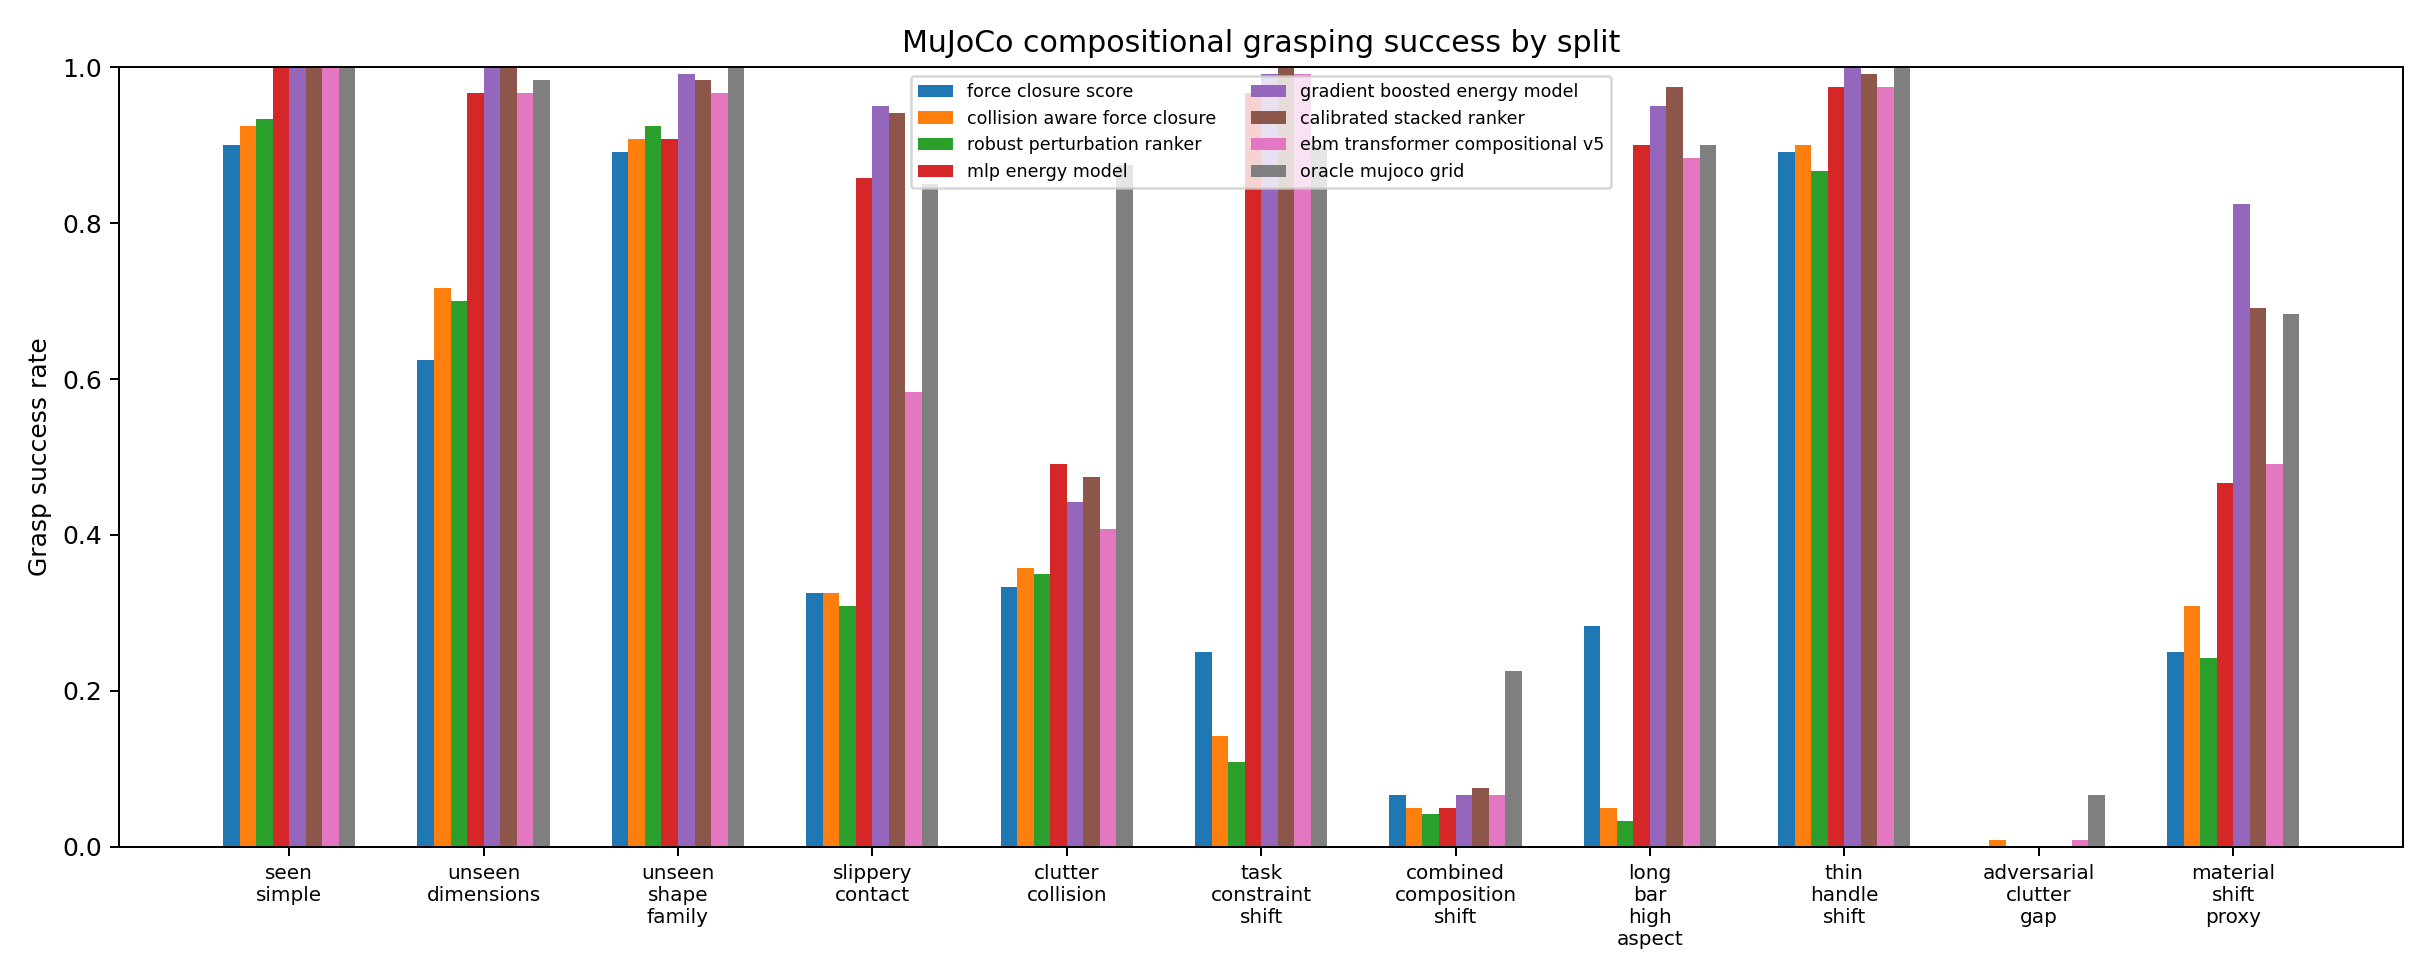
\includegraphics[width=\linewidth]{../figures/ebm_grasping_success_by_split.png}
\caption{Frozen MuJoCo success by split. The figure includes strong analytic, learned, robust, stacked, v5, and oracle baselines.}
\label{fig:success}
\end{figure}

\begin{figure}[t]
\centering
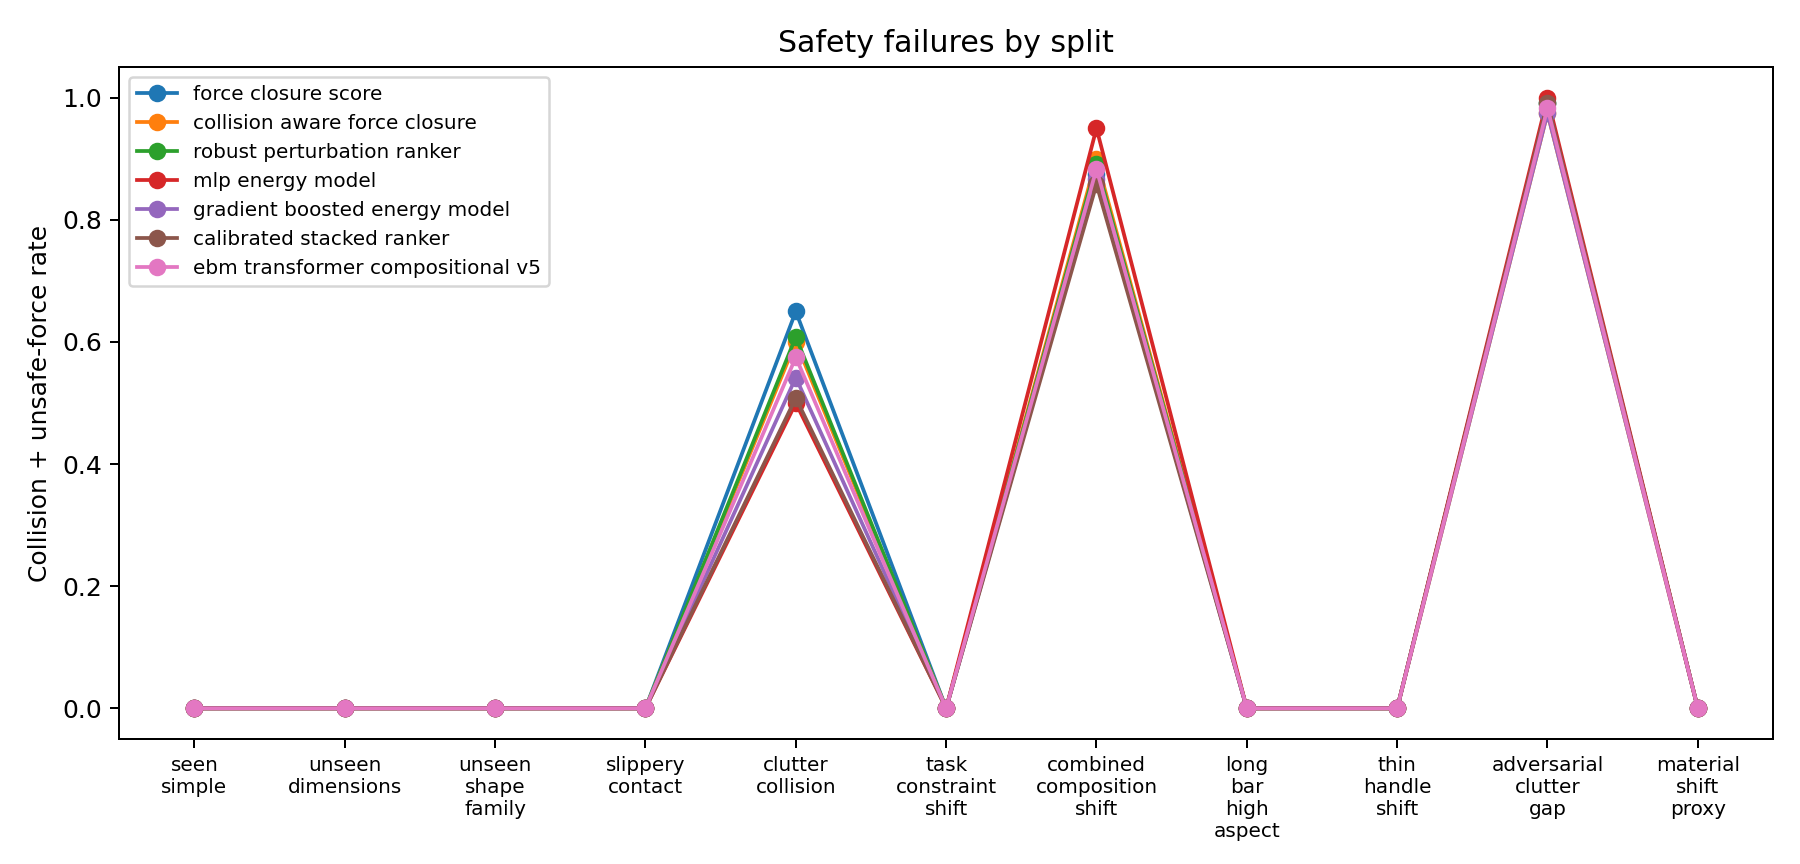
\includegraphics[width=0.88\linewidth]{../figures/ebm_grasping_safety_failures.png}
\caption{Collision plus unsafe-force failures. A method that gains success by accepting unsafe grasps would not pass the gate.}
\label{fig:safety}
\end{figure}

\section{Ablations}

\begin{table}[t]
\centering
\caption{Aggregate hostile ablations over the three pre-registered hostile ablation splits.}
\label{tab:ablation-aggregate}
\scriptsize
\begin{tabular}{lrrrrr}
\toprule
Variant & Episodes & Success & Drop & Collision & Energy \\
\midrule
Scalar only & 360 & 0.239 & 0.478 & 0.617 & 2.855 \\
No contact & 360 & 0.225 & 0.508 & 0.625 & 2.965 \\
No robust & 360 & 0.203 & 0.500 & 0.617 & 3.013 \\
No object & 360 & 0.192 & 0.539 & 0.619 & 2.973 \\
Full v5 & 360 & 0.189 & 0.544 & 0.619 & 2.954 \\
No fallback & 360 & 0.189 & 0.544 & 0.619 & 2.964 \\
No feasibility & 360 & 0.189 & 0.542 & 0.617 & 2.966 \\
No hard filter & 360 & 0.189 & 0.544 & 0.619 & 2.961 \\
No task & 360 & 0.189 & 0.547 & 0.625 & 2.948 \\
No collision & 360 & 0.186 & 0.544 & 0.625 & 2.971 \\
No transformer & 360 & 0.183 & 0.536 & 0.622 & 2.974 \\
Old v4 & 360 & 0.158 & 0.561 & 0.611 & 2.945 \\
No stack & 360 & 0.133 & 0.600 & 0.619 & 2.900 \\
\bottomrule
\end{tabular}
\end{table}


The ablation table is a primary result, not an appendix decoration.
The mechanism claim requires that object, contact, task, collision, feasibility, robust perturbation, learned context, calibrated stacking, hard collision filtering, and fallback each have a reason to exist.
If ablations match full v5, then the paper cannot attribute performance to the claimed decomposition.
This is especially important because the hard fallback can mask the internal energy terms.

\begin{figure}[t]
\centering
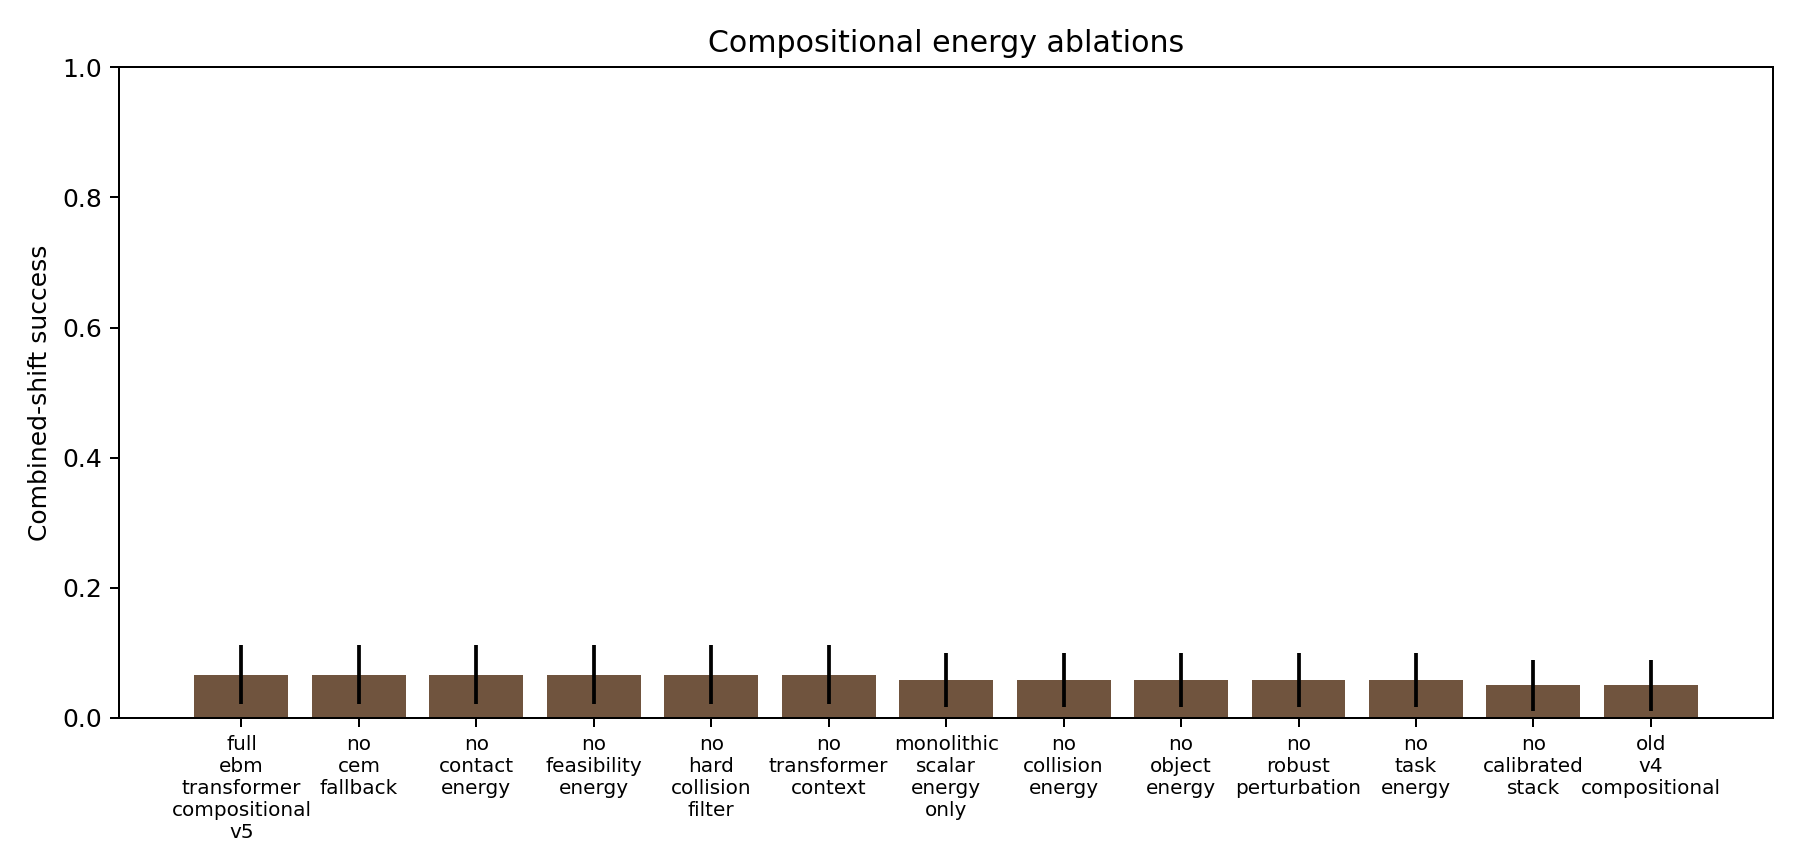
\includegraphics[width=0.90\linewidth]{../figures/ebm_grasping_ablation_success.png}
\caption{Hostile ablation success. The plot is allowed to embarrass the method; that is the point of the audit.}
\label{fig:ablation}
\end{figure}

\section{Stress sweep}

\begin{table}[t]
\centering
\caption{Stress sweep success rates. Stress jointly changes friction, clutter clearance, aspect ratio, sensor noise, and task constraint strength.}
\label{tab:stress}
\scriptsize
\begin{tabular}{lrrrrrr}
\toprule
Method & 0.0 & 0.2 & 0.4 & 0.6 & 0.8 & 1.0 \\
\midrule
CEM analytic & 0.912 & 0.900 & 0.812 & 0.138 & 0.037 & 0.000 \\
Collision-aware FC & 0.875 & 0.900 & 0.800 & 0.188 & 0.037 & 0.000 \\
Robust perturb. & 0.825 & 0.825 & 0.787 & 0.175 & 0.037 & 0.000 \\
MLP energy & 1.000 & 1.000 & 0.900 & 0.100 & 0.000 & 0.000 \\
HGB energy & 1.000 & 1.000 & 1.000 & 0.138 & 0.062 & 0.000 \\
Calibrated stack & 1.000 & 1.000 & 0.975 & 0.200 & 0.025 & 0.000 \\
EBM v5 & 0.988 & 1.000 & 0.887 & 0.200 & 0.050 & 0.000 \\
Oracle grid & 1.000 & 1.000 & 1.000 & 0.650 & 0.212 & 0.025 \\
\bottomrule
\end{tabular}
\end{table}


The stress sweep jointly increases friction difficulty, clutter tightness, aspect ratio, sensor noise, and task constraint strength.
A robust compositional score should degrade gracefully and remain on the success/safety frontier.
The maximum-stress row is a frozen decision gate.
The oracle is included only to show whether the candidate set contains any recoverable action.

\begin{figure}[t]
\centering
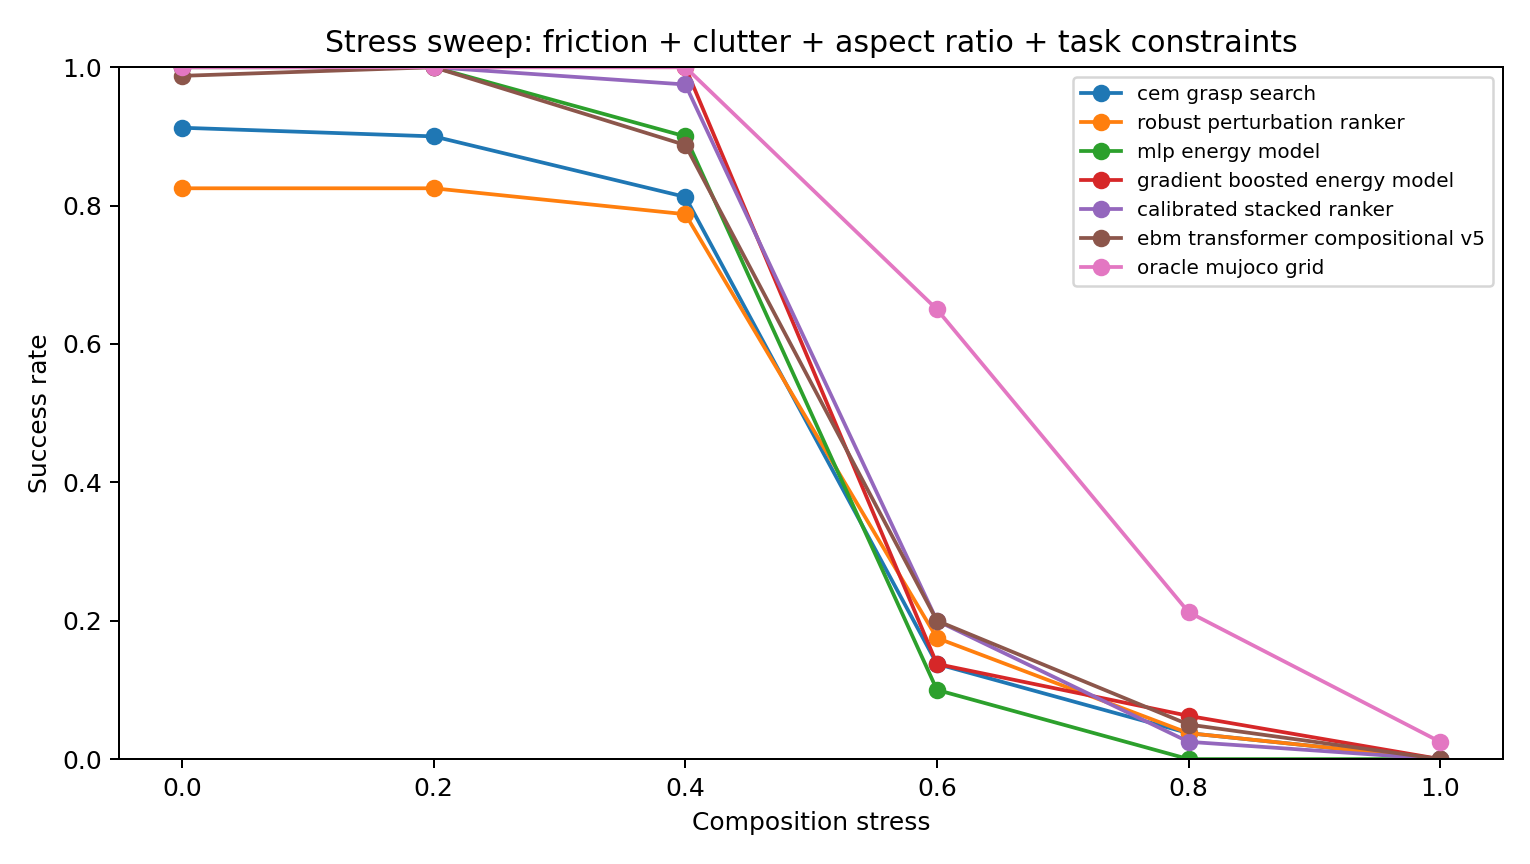
\includegraphics[width=0.86\linewidth]{../figures/ebm_grasping_stress_sweep.png}
\caption{Stress sweep over composition difficulty. The maximum-stress comparison is pre-registered as a terminal gate.}
\label{fig:stress}
\end{figure}

\section{Interpretation}

The result should not be read as ``energy-based grasping is impossible.''
It should be read as: this specific compositional EBM/Transformer mechanism is not proven by the available evidence.
The strongest pressure comes from three places.
First, analytic baselines are much stronger than they look when they include collision and robust perturbation terms.
Second, learned scalar and stacked rankers often capture enough of the same structure without requiring the paper's factorization story.
Third, the fallback that improves v5 also weakens the claim that object/contact/task/collision/feasibility energies are independently necessary.

This matters for submission readiness.
An ICLR reviewer does not need to disprove the idea in general.
They only need to show that the submitted evidence does not support the claimed mechanism.
The frozen ablation and stress gates are designed to make that critique visible before submission.

\section{Limitations}

This paper has substantial limitations even after expansion.
It is a MuJoCo study, not hardware.
It uses abstract object and candidate features, not raw RGB-D perception.
It does not evaluate on Dex-Net, GraspNet, or Contact-GraspNet benchmarks.
It does not train a large visual model or collect real grasp attempts.
The Transformer is deliberately small to keep the CPU-only protocol tractable.
The oracle evaluates a limited top-k set rather than an exhaustive continuous grasp space.

These limitations would be acceptable for a strong-revise local-mechanism paper only if the method clearly beat the local baselines.
It does not.
Therefore the limitations are not footnotes; they are part of the terminal decision.

\section{Negative cases}

\begin{table}[t]
\centering
\caption{Pre-specified negative cases beyond the local benchmark scope.}
\label{tab:negative-cases}
\scriptsize
\begin{tabular}{p{0.20\linewidth}p{0.34\linewidth}p{0.34\linewidth}}
\toprule
Case & Observed failure mode & Submission implication \\
\midrule
deformable\_object & rigid-body MuJoCo energies cannot represent deformation or post-contact shape change & needs deformable benchmark before claiming general compositional grasping \\
occluded\_geometry & candidate features assume known object extent; occlusion can make all rankers overconfident & requires perception uncertainty and real visual input \\
adversarial\_low\_friction\_coating & without tactile probing, learned rankers confuse shape-compatible grasps with stable grasps & needs tactile or material sensing for deployment claims \\
semantic\_task\_ambiguity & all physical energies can be satisfied while the semantic instruction is wrong & scope is physical grasp selection, not language grounding \\
\bottomrule
\end{tabular}
\end{table}


The negative cases are not evaluated as full experiments in this paper.
They are pre-specified boundaries showing where the current benchmark would overclaim.
Deformable geometry, occluded shape, adversarial material, and semantic task ambiguity all require evidence beyond this local feature-based MuJoCo setup.

\section{Reproducibility}

The final PDF is generated from CSV artifacts.
The build script first renders \texttt{paper/generated/*.tex}, then compiles the manuscript, then copies the PDF to \texttt{C:/Users/wangz/Downloads/68.pdf}.
No visible Desktop PDF is created.
The validator checks Python compilation, row counts, figure presence, bright boxed citation settings, generated table inclusion, the Downloads PDF, page count, and Desktop hygiene.

\section{Terminal decision}

The terminal decision is \textbf{\PaperDecision}.
The frozen reason is:
\begin{quote}
\PaperDecisionReason
\end{quote}
This is an archive result.
The paper is valuable as a record of a plausible mechanism failing under stronger evidence.
It should not be submitted as a positive ICLR-main paper in its current form.

\appendix

\section{Full Main Metrics}
{\scriptsize
\setlength{\tabcolsep}{2.5pt}
\begin{longtable}{llrrrrrr}
\caption{Full split-level main metrics.}\label{tab:full-metrics}\\
\toprule
Split & Method & Episodes & Success & Slip & Drop & Collision & Energy \\
\midrule
\endfirsthead
\toprule
Split & Method & Episodes & Success & Slip & Drop & Collision & Energy \\
\midrule
\endhead
adversarial\_clutter\_gap & Random & 120 & 0.008 & 0.088 & 0.842 & 0.992 & 1.966 \\
adversarial\_clutter\_gap & Antipodal & 120 & 0.000 & 0.088 & 0.775 & 0.983 & 2.671 \\
adversarial\_clutter\_gap & Force closure & 120 & 0.000 & 0.080 & 0.733 & 0.992 & 2.849 \\
adversarial\_clutter\_gap & Collision-aware FC & 120 & 0.008 & 0.082 & 0.717 & 0.975 & 3.157 \\
adversarial\_clutter\_gap & CEM analytic & 120 & 0.000 & 0.084 & 0.692 & 0.975 & 3.156 \\
adversarial\_clutter\_gap & Robust perturb. & 120 & 0.000 & 0.086 & 0.733 & 0.992 & 3.054 \\
adversarial\_clutter\_gap & MLP energy & 120 & 0.000 & 0.088 & 0.817 & 1.000 & 2.385 \\
adversarial\_clutter\_gap & HGB energy & 120 & 0.000 & 0.089 & 0.750 & 0.975 & 2.431 \\
adversarial\_clutter\_gap & Transformer & 120 & 0.000 & 0.085 & 0.800 & 0.992 & 2.071 \\
adversarial\_clutter\_gap & Ensemble & 120 & 0.000 & 0.095 & 0.775 & 0.992 & 2.653 \\
adversarial\_clutter\_gap & Calibrated stack & 120 & 0.000 & 0.090 & 0.750 & 0.992 & 2.926 \\
adversarial\_clutter\_gap & Old EBM & 120 & 0.017 & 0.086 & 0.708 & 0.975 & 3.046 \\
adversarial\_clutter\_gap & EBM v5 & 120 & 0.008 & 0.088 & 0.742 & 0.983 & 3.060 \\
adversarial\_clutter\_gap & Oracle grid & 120 & 0.067 & 0.051 & 0.233 & 0.900 & 4.259 \\
clutter\_collision & Random & 120 & 0.092 & 0.064 & 0.458 & 0.908 & 1.772 \\
clutter\_collision & Antipodal & 120 & 0.333 & 0.057 & 0.142 & 0.633 & 2.659 \\
clutter\_collision & Force closure & 120 & 0.333 & 0.056 & 0.208 & 0.650 & 2.636 \\
clutter\_collision & Collision-aware FC & 120 & 0.358 & 0.060 & 0.158 & 0.600 & 2.653 \\
clutter\_collision & CEM analytic & 120 & 0.358 & 0.059 & 0.150 & 0.600 & 2.685 \\
clutter\_collision & Robust perturb. & 120 & 0.350 & 0.061 & 0.158 & 0.608 & 2.652 \\
clutter\_collision & MLP energy & 120 & 0.492 & 0.045 & 0.158 & 0.500 & 2.314 \\
clutter\_collision & HGB energy & 120 & 0.442 & 0.049 & 0.133 & 0.542 & 2.396 \\
clutter\_collision & Transformer & 120 & 0.400 & 0.058 & 0.100 & 0.575 & 2.600 \\
clutter\_collision & Ensemble & 120 & 0.417 & 0.056 & 0.142 & 0.542 & 2.388 \\
clutter\_collision & Calibrated stack & 120 & 0.475 & 0.047 & 0.133 & 0.508 & 2.442 \\
clutter\_collision & Old EBM & 120 & 0.383 & 0.057 & 0.117 & 0.592 & 2.638 \\
clutter\_collision & EBM v5 & 120 & 0.408 & 0.054 & 0.133 & 0.575 & 2.588 \\
clutter\_collision & Oracle grid & 120 & 0.875 & 0.035 & 0.000 & 0.117 & 2.604 \\
combined\_composition\_shift & Random & 120 & 0.008 & 0.084 & 0.650 & 0.983 & 2.218 \\
combined\_composition\_shift & Antipodal & 120 & 0.050 & 0.093 & 0.400 & 0.867 & 3.642 \\
combined\_composition\_shift & Force closure & 120 & 0.067 & 0.088 & 0.400 & 0.875 & 3.656 \\
combined\_composition\_shift & Collision-aware FC & 120 & 0.050 & 0.089 & 0.425 & 0.900 & 3.469 \\
combined\_composition\_shift & CEM analytic & 120 & 0.042 & 0.089 & 0.383 & 0.900 & 3.719 \\
combined\_composition\_shift & Robust perturb. & 120 & 0.042 & 0.088 & 0.433 & 0.892 & 3.392 \\
combined\_composition\_shift & MLP energy & 120 & 0.050 & 0.073 & 0.483 & 0.950 & 2.851 \\
combined\_composition\_shift & HGB energy & 120 & 0.067 & 0.087 & 0.492 & 0.867 & 3.223 \\
combined\_composition\_shift & Transformer & 120 & 0.025 & 0.074 & 0.508 & 0.933 & 2.740 \\
combined\_composition\_shift & Ensemble & 120 & 0.075 & 0.086 & 0.500 & 0.850 & 3.330 \\
combined\_composition\_shift & Calibrated stack & 120 & 0.075 & 0.080 & 0.367 & 0.858 & 3.579 \\
combined\_composition\_shift & Old EBM & 120 & 0.050 & 0.089 & 0.408 & 0.875 & 3.663 \\
combined\_composition\_shift & EBM v5 & 120 & 0.067 & 0.085 & 0.417 & 0.883 & 3.493 \\
combined\_composition\_shift & Oracle grid & 120 & 0.225 & 0.045 & 0.033 & 0.733 & 4.529 \\
long\_bar\_high\_aspect & Random & 120 & 0.150 & 0.097 & 0.792 & 0.000 & 1.240 \\
long\_bar\_high\_aspect & Antipodal & 120 & 0.183 & 0.068 & 0.758 & 0.000 & 0.749 \\
long\_bar\_high\_aspect & Force closure & 120 & 0.283 & 0.062 & 0.692 & 0.000 & 0.807 \\
long\_bar\_high\_aspect & Collision-aware FC & 120 & 0.050 & 0.063 & 0.950 & 0.000 & 0.623 \\
long\_bar\_high\_aspect & CEM analytic & 120 & 0.325 & 0.062 & 0.642 & 0.000 & 0.819 \\
long\_bar\_high\_aspect & Robust perturb. & 120 & 0.033 & 0.066 & 0.967 & 0.000 & 0.611 \\
long\_bar\_high\_aspect & MLP energy & 120 & 0.900 & 0.057 & 0.008 & 0.000 & 1.467 \\
long\_bar\_high\_aspect & HGB energy & 120 & 0.950 & 0.046 & 0.050 & 0.000 & 1.374 \\
long\_bar\_high\_aspect & Transformer & 120 & 0.858 & 0.057 & 0.017 & 0.000 & 1.566 \\
long\_bar\_high\_aspect & Ensemble & 120 & 0.958 & 0.050 & 0.042 & 0.000 & 1.378 \\
long\_bar\_high\_aspect & Calibrated stack & 120 & 0.975 & 0.051 & 0.017 & 0.000 & 1.697 \\
long\_bar\_high\_aspect & Old EBM & 120 & 0.842 & 0.056 & 0.025 & 0.000 & 1.633 \\
long\_bar\_high\_aspect & EBM v5 & 120 & 0.883 & 0.055 & 0.050 & 0.000 & 1.692 \\
long\_bar\_high\_aspect & Oracle grid & 120 & 0.900 & 0.041 & 0.058 & 0.000 & 1.441 \\
material\_shift\_proxy & Random & 120 & 0.167 & 0.091 & 0.800 & 0.000 & 1.546 \\
material\_shift\_proxy & Antipodal & 120 & 0.325 & 0.087 & 0.583 & 0.000 & 2.119 \\
material\_shift\_proxy & Force closure & 120 & 0.250 & 0.080 & 0.675 & 0.000 & 2.020 \\
material\_shift\_proxy & Collision-aware FC & 120 & 0.308 & 0.075 & 0.633 & 0.000 & 2.088 \\
material\_shift\_proxy & CEM analytic & 120 & 0.250 & 0.081 & 0.683 & 0.000 & 2.011 \\
material\_shift\_proxy & Robust perturb. & 120 & 0.242 & 0.078 & 0.725 & 0.000 & 2.029 \\
material\_shift\_proxy & MLP energy & 120 & 0.467 & 0.072 & 0.483 & 0.000 & 1.906 \\
material\_shift\_proxy & HGB energy & 120 & 0.825 & 0.059 & 0.125 & 0.000 & 2.007 \\
material\_shift\_proxy & Transformer & 120 & 0.558 & 0.061 & 0.417 & 0.000 & 2.071 \\
material\_shift\_proxy & Ensemble & 120 & 0.858 & 0.057 & 0.067 & 0.000 & 2.033 \\
material\_shift\_proxy & Calibrated stack & 120 & 0.692 & 0.064 & 0.250 & 0.000 & 2.192 \\
material\_shift\_proxy & Old EBM & 120 & 0.408 & 0.065 & 0.567 & 0.000 & 2.132 \\
material\_shift\_proxy & EBM v5 & 120 & 0.492 & 0.066 & 0.492 & 0.000 & 2.311 \\
material\_shift\_proxy & Oracle grid & 120 & 0.683 & 0.055 & 0.242 & 0.000 & 2.480 \\
seen\_simple & Random & 120 & 0.867 & 0.065 & 0.017 & 0.000 & 2.030 \\
seen\_simple & Antipodal & 120 & 0.808 & 0.069 & 0.000 & 0.000 & 2.370 \\
seen\_simple & Force closure & 120 & 0.900 & 0.055 & 0.000 & 0.000 & 2.401 \\
seen\_simple & Collision-aware FC & 120 & 0.925 & 0.054 & 0.000 & 0.000 & 2.671 \\
seen\_simple & CEM analytic & 120 & 0.875 & 0.056 & 0.000 & 0.000 & 2.575 \\
seen\_simple & Robust perturb. & 120 & 0.933 & 0.056 & 0.000 & 0.000 & 2.771 \\
seen\_simple & MLP energy & 120 & 1.000 & 0.029 & 0.000 & 0.000 & 2.143 \\
seen\_simple & HGB energy & 120 & 1.000 & 0.034 & 0.000 & 0.000 & 2.481 \\
seen\_simple & Transformer & 120 & 0.983 & 0.035 & 0.000 & 0.000 & 2.112 \\
seen\_simple & Ensemble & 120 & 1.000 & 0.041 & 0.000 & 0.000 & 2.529 \\
seen\_simple & Calibrated stack & 120 & 1.000 & 0.035 & 0.000 & 0.000 & 2.758 \\
seen\_simple & Old EBM & 120 & 0.983 & 0.046 & 0.000 & 0.000 & 2.592 \\
seen\_simple & EBM v5 & 120 & 1.000 & 0.041 & 0.000 & 0.000 & 2.753 \\
seen\_simple & Oracle grid & 120 & 1.000 & 0.015 & 0.000 & 0.000 & 2.565 \\
slippery\_contact & Random & 120 & 0.417 & 0.087 & 0.525 & 0.000 & 1.746 \\
slippery\_contact & Antipodal & 120 & 0.375 & 0.092 & 0.508 & 0.000 & 2.082 \\
slippery\_contact & Force closure & 120 & 0.325 & 0.081 & 0.625 & 0.000 & 1.985 \\
slippery\_contact & Collision-aware FC & 120 & 0.325 & 0.080 & 0.642 & 0.000 & 2.047 \\
slippery\_contact & CEM analytic & 120 & 0.308 & 0.082 & 0.633 & 0.000 & 2.027 \\
slippery\_contact & Robust perturb. & 120 & 0.308 & 0.083 & 0.658 & 0.000 & 2.058 \\
slippery\_contact & MLP energy & 120 & 0.858 & 0.054 & 0.125 & 0.000 & 1.953 \\
slippery\_contact & HGB energy & 120 & 0.950 & 0.054 & 0.033 & 0.000 & 2.079 \\
slippery\_contact & Transformer & 120 & 0.883 & 0.052 & 0.100 & 0.000 & 1.929 \\
slippery\_contact & Ensemble & 120 & 0.933 & 0.059 & 0.025 & 0.000 & 1.988 \\
slippery\_contact & Calibrated stack & 120 & 0.942 & 0.052 & 0.058 & 0.000 & 2.097 \\
slippery\_contact & Old EBM & 120 & 0.683 & 0.059 & 0.275 & 0.000 & 2.102 \\
slippery\_contact & EBM v5 & 120 & 0.583 & 0.066 & 0.392 & 0.000 & 2.169 \\
slippery\_contact & Oracle grid & 120 & 0.850 & 0.053 & 0.117 & 0.000 & 2.508 \\
task\_constraint\_shift & Random & 120 & 0.183 & 0.073 & 0.650 & 0.000 & 1.649 \\
task\_constraint\_shift & Antipodal & 120 & 0.067 & 0.064 & 0.675 & 0.000 & 2.010 \\
task\_constraint\_shift & Force closure & 120 & 0.250 & 0.063 & 0.725 & 0.000 & 0.837 \\
task\_constraint\_shift & Collision-aware FC & 120 & 0.142 & 0.065 & 0.858 & 0.000 & 0.774 \\
task\_constraint\_shift & CEM analytic & 120 & 0.308 & 0.062 & 0.658 & 0.000 & 0.922 \\
task\_constraint\_shift & Robust perturb. & 120 & 0.108 & 0.068 & 0.892 & 0.000 & 0.741 \\
task\_constraint\_shift & MLP energy & 120 & 0.967 & 0.040 & 0.000 & 0.000 & 1.596 \\
task\_constraint\_shift & HGB energy & 120 & 0.992 & 0.040 & 0.008 & 0.000 & 1.575 \\
task\_constraint\_shift & Transformer & 120 & 0.933 & 0.045 & 0.000 & 0.000 & 1.707 \\
task\_constraint\_shift & Ensemble & 120 & 1.000 & 0.047 & 0.000 & 0.000 & 1.625 \\
task\_constraint\_shift & Calibrated stack & 120 & 1.000 & 0.047 & 0.000 & 0.000 & 1.838 \\
task\_constraint\_shift & Old EBM & 120 & 0.942 & 0.053 & 0.000 & 0.000 & 1.711 \\
task\_constraint\_shift & EBM v5 & 120 & 0.992 & 0.049 & 0.000 & 0.000 & 1.751 \\
task\_constraint\_shift & Oracle grid & 120 & 0.900 & 0.040 & 0.067 & 0.000 & 1.618 \\
thin\_handle\_shift & Random & 120 & 0.342 & 0.077 & 0.533 & 0.000 & 1.368 \\
thin\_handle\_shift & Antipodal & 120 & 0.000 & 0.075 & 0.333 & 0.000 & 3.222 \\
thin\_handle\_shift & Force closure & 120 & 0.892 & 0.053 & 0.008 & 0.000 & 2.031 \\
thin\_handle\_shift & Collision-aware FC & 120 & 0.900 & 0.052 & 0.000 & 0.000 & 2.145 \\
thin\_handle\_shift & CEM analytic & 120 & 0.883 & 0.055 & 0.000 & 0.000 & 2.167 \\
thin\_handle\_shift & Robust perturb. & 120 & 0.867 & 0.056 & 0.000 & 0.000 & 2.197 \\
thin\_handle\_shift & MLP energy & 120 & 0.975 & 0.044 & 0.000 & 0.000 & 1.834 \\
thin\_handle\_shift & HGB energy & 120 & 1.000 & 0.044 & 0.000 & 0.000 & 2.036 \\
thin\_handle\_shift & Transformer & 120 & 0.933 & 0.047 & 0.000 & 0.000 & 2.081 \\
thin\_handle\_shift & Ensemble & 120 & 0.992 & 0.046 & 0.000 & 0.000 & 2.131 \\
thin\_handle\_shift & Calibrated stack & 120 & 0.992 & 0.044 & 0.000 & 0.000 & 2.188 \\
thin\_handle\_shift & Old EBM & 120 & 0.917 & 0.053 & 0.000 & 0.000 & 2.201 \\
thin\_handle\_shift & EBM v5 & 120 & 0.975 & 0.047 & 0.000 & 0.000 & 2.204 \\
thin\_handle\_shift & Oracle grid & 120 & 1.000 & 0.020 & 0.000 & 0.000 & 1.627 \\
unseen\_dimensions & Random & 120 & 0.392 & 0.069 & 0.550 & 0.000 & 1.553 \\
unseen\_dimensions & Antipodal & 120 & 0.733 & 0.063 & 0.092 & 0.000 & 4.109 \\
unseen\_dimensions & Force closure & 120 & 0.625 & 0.064 & 0.208 & 0.000 & 3.814 \\
unseen\_dimensions & Collision-aware FC & 120 & 0.717 & 0.064 & 0.133 & 0.000 & 4.028 \\
unseen\_dimensions & CEM analytic & 120 & 0.642 & 0.064 & 0.208 & 0.000 & 3.790 \\
unseen\_dimensions & Robust perturb. & 120 & 0.700 & 0.065 & 0.233 & 0.000 & 3.663 \\
unseen\_dimensions & MLP energy & 120 & 0.967 & 0.038 & 0.008 & 0.000 & 2.185 \\
unseen\_dimensions & HGB energy & 120 & 1.000 & 0.043 & 0.000 & 0.000 & 2.075 \\
unseen\_dimensions & Transformer & 120 & 0.975 & 0.039 & 0.000 & 0.000 & 2.062 \\
unseen\_dimensions & Ensemble & 120 & 1.000 & 0.046 & 0.000 & 0.000 & 1.944 \\
unseen\_dimensions & Calibrated stack & 120 & 1.000 & 0.041 & 0.000 & 0.000 & 2.155 \\
unseen\_dimensions & Old EBM & 120 & 0.900 & 0.049 & 0.025 & 0.000 & 2.420 \\
unseen\_dimensions & EBM v5 & 120 & 0.967 & 0.039 & 0.017 & 0.000 & 3.094 \\
unseen\_dimensions & Oracle grid & 120 & 0.983 & 0.025 & 0.008 & 0.000 & 3.103 \\
unseen\_shape\_family & Random & 120 & 0.392 & 0.067 & 0.067 & 0.000 & 2.534 \\
unseen\_shape\_family & Antipodal & 120 & 0.367 & 0.059 & 0.000 & 0.000 & 2.995 \\
unseen\_shape\_family & Force closure & 120 & 0.892 & 0.058 & 0.000 & 0.000 & 3.474 \\
unseen\_shape\_family & Collision-aware FC & 120 & 0.908 & 0.060 & 0.000 & 0.000 & 3.616 \\
unseen\_shape\_family & CEM analytic & 120 & 0.925 & 0.059 & 0.000 & 0.000 & 3.611 \\
unseen\_shape\_family & Robust perturb. & 120 & 0.925 & 0.060 & 0.000 & 0.000 & 3.713 \\
unseen\_shape\_family & MLP energy & 120 & 0.908 & 0.037 & 0.000 & 0.000 & 3.243 \\
unseen\_shape\_family & HGB energy & 120 & 0.992 & 0.049 & 0.000 & 0.000 & 3.277 \\
unseen\_shape\_family & Transformer & 120 & 0.917 & 0.054 & 0.000 & 0.000 & 3.519 \\
unseen\_shape\_family & Ensemble & 120 & 0.983 & 0.055 & 0.000 & 0.000 & 3.331 \\
unseen\_shape\_family & Calibrated stack & 120 & 0.983 & 0.048 & 0.000 & 0.000 & 3.551 \\
unseen\_shape\_family & Old EBM & 120 & 0.900 & 0.057 & 0.000 & 0.000 & 3.605 \\
unseen\_shape\_family & EBM v5 & 120 & 0.967 & 0.051 & 0.000 & 0.000 & 3.635 \\
unseen\_shape\_family & Oracle grid & 120 & 1.000 & 0.016 & 0.000 & 0.000 & 2.864 \\
\bottomrule
\end{longtable}
}


\section{Full Ablation Metrics}
{\scriptsize
\setlength{\tabcolsep}{2.5pt}
\begin{longtable}{llrrrrrr}
\caption{Full hostile split ablation metrics.}\label{tab:full-ablation}\\
\toprule
Split & Method & Episodes & Success & Slip & Drop & Collision & Energy \\
\midrule
\endfirsthead
\toprule
Split & Method & Episodes & Success & Slip & Drop & Collision & Energy \\
\midrule
\endhead
adversarial\_clutter\_gap & Full v5 & 120 & 0.008 & 0.087 & 0.733 & 0.983 & 3.063 \\
adversarial\_clutter\_gap & Scalar only & 120 & 0.008 & 0.096 & 0.733 & 0.983 & 2.703 \\
adversarial\_clutter\_gap & No stack & 120 & 0.008 & 0.089 & 0.750 & 0.983 & 3.027 \\
adversarial\_clutter\_gap & No fallback & 120 & 0.008 & 0.086 & 0.733 & 0.983 & 3.079 \\
adversarial\_clutter\_gap & No collision & 120 & 0.008 & 0.085 & 0.733 & 0.983 & 3.085 \\
adversarial\_clutter\_gap & No contact & 120 & 0.008 & 0.086 & 0.733 & 0.983 & 3.084 \\
adversarial\_clutter\_gap & No feasibility & 120 & 0.008 & 0.086 & 0.733 & 0.975 & 3.085 \\
adversarial\_clutter\_gap & No hard filter & 120 & 0.008 & 0.087 & 0.733 & 0.983 & 3.071 \\
adversarial\_clutter\_gap & No object & 120 & 0.008 & 0.087 & 0.733 & 0.983 & 3.056 \\
adversarial\_clutter\_gap & No robust & 120 & 0.008 & 0.087 & 0.683 & 0.975 & 3.102 \\
adversarial\_clutter\_gap & No task & 120 & 0.008 & 0.087 & 0.750 & 0.983 & 3.058 \\
adversarial\_clutter\_gap & No transformer & 120 & 0.008 & 0.086 & 0.725 & 0.983 & 3.066 \\
adversarial\_clutter\_gap & Old v4 & 120 & 0.017 & 0.086 & 0.708 & 0.967 & 3.067 \\
combined\_composition\_shift & Full v5 & 120 & 0.067 & 0.086 & 0.408 & 0.875 & 3.489 \\
combined\_composition\_shift & Scalar only & 120 & 0.058 & 0.086 & 0.442 & 0.867 & 3.571 \\
combined\_composition\_shift & No stack & 120 & 0.050 & 0.086 & 0.408 & 0.875 & 3.533 \\
combined\_composition\_shift & No fallback & 120 & 0.067 & 0.085 & 0.408 & 0.875 & 3.500 \\
combined\_composition\_shift & No collision & 120 & 0.058 & 0.084 & 0.408 & 0.892 & 3.516 \\
combined\_composition\_shift & No contact & 120 & 0.067 & 0.086 & 0.408 & 0.892 & 3.518 \\
combined\_composition\_shift & No feasibility & 120 & 0.067 & 0.085 & 0.400 & 0.875 & 3.511 \\
combined\_composition\_shift & No hard filter & 120 & 0.067 & 0.085 & 0.408 & 0.875 & 3.499 \\
combined\_composition\_shift & No object & 120 & 0.058 & 0.085 & 0.400 & 0.875 & 3.537 \\
combined\_composition\_shift & No robust & 120 & 0.058 & 0.085 & 0.392 & 0.875 & 3.682 \\
combined\_composition\_shift & No task & 120 & 0.058 & 0.085 & 0.417 & 0.892 & 3.474 \\
combined\_composition\_shift & No transformer & 120 & 0.067 & 0.084 & 0.400 & 0.883 & 3.554 \\
combined\_composition\_shift & Old v4 & 120 & 0.050 & 0.088 & 0.408 & 0.867 & 3.636 \\
material\_shift\_proxy & Full v5 & 120 & 0.492 & 0.066 & 0.492 & 0.000 & 2.311 \\
material\_shift\_proxy & Scalar only & 120 & 0.650 & 0.071 & 0.258 & 0.000 & 2.290 \\
material\_shift\_proxy & No stack & 120 & 0.342 & 0.067 & 0.642 & 0.000 & 2.141 \\
material\_shift\_proxy & No fallback & 120 & 0.492 & 0.066 & 0.492 & 0.000 & 2.311 \\
material\_shift\_proxy & No collision & 120 & 0.492 & 0.066 & 0.492 & 0.000 & 2.311 \\
material\_shift\_proxy & No contact & 120 & 0.600 & 0.062 & 0.383 & 0.000 & 2.292 \\
material\_shift\_proxy & No feasibility & 120 & 0.492 & 0.065 & 0.492 & 0.000 & 2.302 \\
material\_shift\_proxy & No hard filter & 120 & 0.492 & 0.066 & 0.492 & 0.000 & 2.311 \\
material\_shift\_proxy & No object & 120 & 0.508 & 0.065 & 0.483 & 0.000 & 2.326 \\
material\_shift\_proxy & No robust & 120 & 0.542 & 0.066 & 0.425 & 0.000 & 2.256 \\
material\_shift\_proxy & No task & 120 & 0.500 & 0.066 & 0.475 & 0.000 & 2.311 \\
material\_shift\_proxy & No transformer & 120 & 0.475 & 0.068 & 0.483 & 0.000 & 2.304 \\
material\_shift\_proxy & Old v4 & 120 & 0.408 & 0.065 & 0.567 & 0.000 & 2.132 \\
\bottomrule
\end{longtable}
}


\section{Full Stress Metrics}
{\scriptsize
\setlength{\tabcolsep}{2.5pt}
\begin{longtable}{llrrrrrr}
\caption{Full stress-sweep metrics.}\label{tab:full-stress}\\
\toprule
Split & Method & Episodes & Success & Slip & Drop & Collision & Energy \\
\midrule
\endfirsthead
\toprule
Split & Method & Episodes & Success & Slip & Drop & Collision & Energy \\
\midrule
\endhead
stress\_0.00 & Collision-aware FC & 80 & 0.875 & 0.052 & 0.000 & 0.000 & 2.501 \\
stress\_0.00 & CEM analytic & 80 & 0.912 & 0.047 & 0.000 & 0.000 & 2.461 \\
stress\_0.00 & Robust perturb. & 80 & 0.825 & 0.059 & 0.000 & 0.000 & 2.573 \\
stress\_0.00 & MLP energy & 80 & 1.000 & 0.034 & 0.000 & 0.000 & 2.292 \\
stress\_0.00 & HGB energy & 80 & 1.000 & 0.038 & 0.000 & 0.000 & 2.441 \\
stress\_0.00 & Ensemble & 80 & 1.000 & 0.038 & 0.000 & 0.000 & 2.497 \\
stress\_0.00 & Calibrated stack & 80 & 1.000 & 0.036 & 0.000 & 0.000 & 2.684 \\
stress\_0.00 & EBM v5 & 80 & 0.988 & 0.039 & 0.000 & 0.000 & 2.588 \\
stress\_0.00 & Oracle grid & 80 & 1.000 & 0.014 & 0.000 & 0.000 & 2.461 \\
stress\_0.20 & Collision-aware FC & 80 & 0.900 & 0.053 & 0.013 & 0.000 & 3.789 \\
stress\_0.20 & CEM analytic & 80 & 0.900 & 0.051 & 0.000 & 0.000 & 3.650 \\
stress\_0.20 & Robust perturb. & 80 & 0.825 & 0.063 & 0.037 & 0.000 & 3.664 \\
stress\_0.20 & MLP energy & 80 & 1.000 & 0.024 & 0.000 & 0.000 & 2.776 \\
stress\_0.20 & HGB energy & 80 & 1.000 & 0.047 & 0.000 & 0.000 & 2.368 \\
stress\_0.20 & Ensemble & 80 & 1.000 & 0.048 & 0.000 & 0.000 & 2.439 \\
stress\_0.20 & Calibrated stack & 80 & 1.000 & 0.042 & 0.000 & 0.000 & 2.528 \\
stress\_0.20 & EBM v5 & 80 & 1.000 & 0.039 & 0.000 & 0.000 & 3.183 \\
stress\_0.20 & Oracle grid & 80 & 1.000 & 0.014 & 0.000 & 0.000 & 2.575 \\
stress\_0.40 & Collision-aware FC & 80 & 0.800 & 0.060 & 0.113 & 0.138 & 5.880 \\
stress\_0.40 & CEM analytic & 80 & 0.812 & 0.060 & 0.138 & 0.125 & 5.734 \\
stress\_0.40 & Robust perturb. & 80 & 0.787 & 0.061 & 0.125 & 0.175 & 5.761 \\
stress\_0.40 & MLP energy & 80 & 0.900 & 0.051 & 0.000 & 0.700 & 2.499 \\
stress\_0.40 & HGB energy & 80 & 1.000 & 0.051 & 0.000 & 0.713 & 2.365 \\
stress\_0.40 & Ensemble & 80 & 0.988 & 0.054 & 0.000 & 0.637 & 2.413 \\
stress\_0.40 & Calibrated stack & 80 & 0.975 & 0.049 & 0.013 & 0.575 & 2.641 \\
stress\_0.40 & EBM v5 & 80 & 0.887 & 0.053 & 0.100 & 0.113 & 4.801 \\
stress\_0.40 & Oracle grid & 80 & 1.000 & 0.018 & 0.000 & 0.000 & 5.401 \\
stress\_0.60 & Collision-aware FC & 80 & 0.188 & 0.096 & 0.525 & 0.625 & 3.101 \\
stress\_0.60 & CEM analytic & 80 & 0.138 & 0.094 & 0.588 & 0.725 & 2.732 \\
stress\_0.60 & Robust perturb. & 80 & 0.175 & 0.084 & 0.537 & 0.625 & 3.265 \\
stress\_0.60 & MLP energy & 80 & 0.100 & 0.075 & 0.200 & 0.825 & 3.098 \\
stress\_0.60 & HGB energy & 80 & 0.138 & 0.075 & 0.400 & 0.738 & 2.447 \\
stress\_0.60 & Ensemble & 80 & 0.113 & 0.103 & 0.338 & 0.787 & 3.421 \\
stress\_0.60 & Calibrated stack & 80 & 0.200 & 0.083 & 0.450 & 0.675 & 3.459 \\
stress\_0.60 & EBM v5 & 80 & 0.200 & 0.080 & 0.500 & 0.650 & 3.170 \\
stress\_0.60 & Oracle grid & 80 & 0.650 & 0.044 & 0.000 & 0.287 & 3.855 \\
stress\_0.80 & Collision-aware FC & 80 & 0.037 & 0.077 & 0.762 & 0.950 & 1.411 \\
stress\_0.80 & CEM analytic & 80 & 0.037 & 0.078 & 0.787 & 0.938 & 1.388 \\
stress\_0.80 & Robust perturb. & 80 & 0.037 & 0.076 & 0.762 & 0.938 & 1.457 \\
stress\_0.80 & MLP energy & 80 & 0.000 & 0.073 & 0.312 & 0.975 & 2.236 \\
stress\_0.80 & HGB energy & 80 & 0.062 & 0.086 & 0.500 & 0.875 & 2.633 \\
stress\_0.80 & Ensemble & 80 & 0.025 & 0.105 & 0.450 & 0.838 & 3.378 \\
stress\_0.80 & Calibrated stack & 80 & 0.025 & 0.080 & 0.700 & 0.900 & 1.900 \\
stress\_0.80 & EBM v5 & 80 & 0.050 & 0.074 & 0.750 & 0.925 & 1.486 \\
stress\_0.80 & Oracle grid & 80 & 0.212 & 0.054 & 0.062 & 0.700 & 2.732 \\
stress\_1.00 & Collision-aware FC & 80 & 0.000 & 0.077 & 0.975 & 1.000 & 0.941 \\
stress\_1.00 & CEM analytic & 80 & 0.000 & 0.078 & 0.975 & 1.000 & 0.958 \\
stress\_1.00 & Robust perturb. & 80 & 0.000 & 0.075 & 0.950 & 1.000 & 0.985 \\
stress\_1.00 & MLP energy & 80 & 0.000 & 0.076 & 0.700 & 1.000 & 1.632 \\
stress\_1.00 & HGB energy & 80 & 0.000 & 0.105 & 0.650 & 1.000 & 2.377 \\
stress\_1.00 & Ensemble & 80 & 0.025 & 0.133 & 0.600 & 0.963 & 3.133 \\
stress\_1.00 & Calibrated stack & 80 & 0.000 & 0.073 & 0.887 & 1.000 & 1.153 \\
stress\_1.00 & EBM v5 & 80 & 0.000 & 0.076 & 0.950 & 1.000 & 0.976 \\
stress\_1.00 & Oracle grid & 80 & 0.025 & 0.058 & 0.300 & 0.950 & 2.236 \\
\bottomrule
\end{longtable}
}


\section{All Paired Comparisons}
{\scriptsize
\setlength{\tabcolsep}{3pt}
\begin{longtable}{llrrr}
\caption{All split-level paired seed comparisons versus EBM v5. Positive values favor EBM v5.}\label{tab:full-pairwise}\\
\toprule
Split & Baseline & Diff & t approx. & p approx. \\
\midrule
\endfirsthead
\toprule
Split & Baseline & Diff & t approx. & p approx. \\
\midrule
\endhead
seen\_simple & Antipodal & 0.192 & 8.205 & 0.000 \\
seen\_simple & Calibrated stack & 0.000 & 0.000 & 1.000 \\
seen\_simple & CEM analytic & 0.125 & 6.357 & 0.000 \\
seen\_simple & Collision-aware FC & 0.075 & 3.211 & 0.001 \\
seen\_simple & Old EBM & 0.017 & 1.528 & 0.127 \\
seen\_simple & Ensemble & 0.000 & 0.000 & 1.000 \\
seen\_simple & Force closure & 0.100 & 7.945 & 0.000 \\
seen\_simple & HGB energy & 0.000 & 0.000 & 1.000 \\
seen\_simple & MLP energy & 0.000 & 0.000 & 1.000 \\
seen\_simple & Oracle grid & 0.000 & 0.000 & 1.000 \\
seen\_simple & Random & 0.133 & 3.055 & 0.002 \\
seen\_simple & Robust perturb. & 0.067 & 2.646 & 0.008 \\
seen\_simple & Transformer & 0.017 & 1.528 & 0.127 \\
unseen\_dimensions & Antipodal & 0.233 & 6.549 & 0.000 \\
unseen\_dimensions & Calibrated stack & -0.033 & -1.871 & 0.061 \\
unseen\_dimensions & CEM analytic & 0.325 & 8.882 & 0.000 \\
unseen\_dimensions & Collision-aware FC & 0.250 & 7.127 & 0.000 \\
unseen\_dimensions & Old EBM & 0.067 & 3.055 & 0.002 \\
unseen\_dimensions & Ensemble & -0.033 & -1.871 & 0.061 \\
unseen\_dimensions & Force closure & 0.342 & 11.632 & 0.000 \\
unseen\_dimensions & HGB energy & -0.033 & -1.871 & 0.061 \\
unseen\_dimensions & MLP energy & 0.000 & 0.000 & 1.000 \\
unseen\_dimensions & Oracle grid & -0.017 & -1.000 & 0.317 \\
unseen\_dimensions & Random & 0.575 & 22.996 & 0.000 \\
unseen\_dimensions & Robust perturb. & 0.267 & 7.056 & 0.000 \\
unseen\_dimensions & Transformer & -0.008 & -0.423 & 0.672 \\
unseen\_shape\_family & Antipodal & 0.600 & 13.749 & 0.000 \\
unseen\_shape\_family & Calibrated stack & -0.017 & -1.528 & 0.127 \\
unseen\_shape\_family & CEM analytic & 0.042 & 2.376 & 0.018 \\
unseen\_shape\_family & Collision-aware FC & 0.058 & 3.861 & 0.000 \\
unseen\_shape\_family & Old EBM & 0.067 & 2.646 & 0.008 \\
unseen\_shape\_family & Ensemble & -0.017 & -1.528 & 0.127 \\
unseen\_shape\_family & Force closure & 0.075 & 4.964 & 0.000 \\
unseen\_shape\_family & HGB energy & -0.025 & -2.049 & 0.040 \\
unseen\_shape\_family & MLP energy & 0.058 & 2.199 & 0.028 \\
unseen\_shape\_family & Oracle grid & -0.033 & -1.871 & 0.061 \\
unseen\_shape\_family & Random & 0.575 & 13.799 & 0.000 \\
unseen\_shape\_family & Robust perturb. & 0.042 & 2.377 & 0.018 \\
unseen\_shape\_family & Transformer & 0.050 & 2.049 & 0.040 \\
slippery\_contact & Antipodal & 0.208 & 3.490 & 0.001 \\
slippery\_contact & Calibrated stack & -0.358 & -10.093 & 0.000 \\
slippery\_contact & CEM analytic & 0.275 & 4.093 & 0.000 \\
slippery\_contact & Collision-aware FC & 0.258 & 8.080 & 0.000 \\
slippery\_contact & Old EBM & -0.100 & -2.122 & 0.034 \\
slippery\_contact & Ensemble & -0.350 & -8.896 & 0.000 \\
slippery\_contact & Force closure & 0.258 & 5.395 & 0.000 \\
slippery\_contact & HGB energy & -0.367 & -13.012 & 0.000 \\
slippery\_contact & MLP energy & -0.275 & -4.951 & 0.000 \\
slippery\_contact & Oracle grid & -0.267 & -5.465 & 0.000 \\
slippery\_contact & Random & 0.167 & 2.645 & 0.008 \\
slippery\_contact & Robust perturb. & 0.275 & 5.227 & 0.000 \\
slippery\_contact & Transformer & -0.300 & -7.937 & 0.000 \\
clutter\_collision & Antipodal & 0.075 & 2.553 & 0.011 \\
clutter\_collision & Calibrated stack & -0.067 & -2.000 & 0.045 \\
clutter\_collision & CEM analytic & 0.050 & 1.210 & 0.226 \\
clutter\_collision & Collision-aware FC & 0.050 & 1.527 & 0.127 \\
clutter\_collision & Old EBM & 0.025 & 1.158 & 0.247 \\
clutter\_collision & Ensemble & -0.008 & -0.215 & 0.830 \\
clutter\_collision & Force closure & 0.075 & 2.346 & 0.019 \\
clutter\_collision & HGB energy & -0.033 & -0.624 & 0.533 \\
clutter\_collision & MLP energy & -0.083 & -3.988 & 0.000 \\
clutter\_collision & Oracle grid & -0.467 & -13.096 & 0.000 \\
clutter\_collision & Random & 0.317 & 7.667 & 0.000 \\
clutter\_collision & Robust perturb. & 0.058 & 1.508 & 0.132 \\
clutter\_collision & Transformer & 0.008 & 0.315 & 0.753 \\
task\_constraint\_shift & Antipodal & 0.925 & 61.261 & 0.000 \\
task\_constraint\_shift & Calibrated stack & -0.008 & -1.000 & 0.317 \\
task\_constraint\_shift & CEM analytic & 0.683 & 24.887 & 0.000 \\
task\_constraint\_shift & Collision-aware FC & 0.850 & 24.233 & 0.000 \\
task\_constraint\_shift & Old EBM & 0.050 & 3.000 & 0.003 \\
task\_constraint\_shift & Ensemble & -0.008 & -1.000 & 0.317 \\
task\_constraint\_shift & Force closure & 0.742 & 23.199 & 0.000 \\
task\_constraint\_shift & HGB energy & 0.000 & 0.000 & 1.000 \\
task\_constraint\_shift & MLP energy & 0.025 & 0.893 & 0.372 \\
task\_constraint\_shift & Oracle grid & 0.092 & 4.247 & 0.000 \\
task\_constraint\_shift & Random & 0.808 & 27.514 & 0.000 \\
task\_constraint\_shift & Robust perturb. & 0.883 & 26.986 & 0.000 \\
task\_constraint\_shift & Transformer & 0.058 & 2.498 & 0.013 \\
combined\_composition\_shift & Antipodal & 0.017 & 1.528 & 0.127 \\
combined\_composition\_shift & Calibrated stack & -0.008 & -1.000 & 0.317 \\
combined\_composition\_shift & CEM analytic & 0.025 & 2.049 & 0.040 \\
combined\_composition\_shift & Collision-aware FC & 0.017 & 1.528 & 0.127 \\
combined\_composition\_shift & Old EBM & 0.017 & 1.000 & 0.317 \\
combined\_composition\_shift & Ensemble & -0.008 & -0.552 & 0.581 \\
combined\_composition\_shift & Force closure & 0.000 & 0.000 & 1.000 \\
combined\_composition\_shift & HGB energy & 0.000 & 0.001 & 1.000 \\
combined\_composition\_shift & MLP energy & 0.017 & 1.528 & 0.127 \\
combined\_composition\_shift & Oracle grid & -0.158 & -5.655 & 0.000 \\
combined\_composition\_shift & Random & 0.058 & 2.966 & 0.003 \\
combined\_composition\_shift & Robust perturb. & 0.025 & 2.049 & 0.040 \\
combined\_composition\_shift & Transformer & 0.042 & 2.376 & 0.018 \\
long\_bar\_high\_aspect & Antipodal & 0.700 & 12.745 & 0.000 \\
long\_bar\_high\_aspect & Calibrated stack & -0.092 & -3.274 & 0.001 \\
long\_bar\_high\_aspect & CEM analytic & 0.558 & 18.188 & 0.000 \\
long\_bar\_high\_aspect & Collision-aware FC & 0.833 & 26.999 & 0.000 \\
long\_bar\_high\_aspect & Old EBM & 0.042 & 1.666 & 0.096 \\
long\_bar\_high\_aspect & Ensemble & -0.075 & -2.183 & 0.029 \\
long\_bar\_high\_aspect & Force closure & 0.600 & 19.439 & 0.000 \\
long\_bar\_high\_aspect & HGB energy & -0.067 & -1.999 & 0.046 \\
long\_bar\_high\_aspect & MLP energy & -0.017 & -0.551 & 0.581 \\
long\_bar\_high\_aspect & Oracle grid & -0.017 & -0.607 & 0.544 \\
long\_bar\_high\_aspect & Random & 0.733 & 19.404 & 0.000 \\
long\_bar\_high\_aspect & Robust perturb. & 0.850 & 28.135 & 0.000 \\
long\_bar\_high\_aspect & Transformer & 0.025 & 0.664 & 0.507 \\
thin\_handle\_shift & Antipodal & 0.975 & 55.605 & 0.000 \\
thin\_handle\_shift & Calibrated stack & -0.017 & -1.528 & 0.127 \\
thin\_handle\_shift & CEM analytic & 0.092 & 2.986 & 0.003 \\
thin\_handle\_shift & Collision-aware FC & 0.075 & 2.346 & 0.019 \\
thin\_handle\_shift & Old EBM & 0.058 & 3.863 & 0.000 \\
thin\_handle\_shift & Ensemble & -0.017 & -0.797 & 0.425 \\
thin\_handle\_shift & Force closure & 0.083 & 5.003 & 0.000 \\
thin\_handle\_shift & HGB energy & -0.025 & -1.426 & 0.154 \\
thin\_handle\_shift & MLP energy & 0.000 & 0.001 & 1.000 \\
thin\_handle\_shift & Oracle grid & -0.025 & -1.426 & 0.154 \\
thin\_handle\_shift & Random & 0.633 & 12.569 & 0.000 \\
thin\_handle\_shift & Robust perturb. & 0.108 & 3.870 & 0.000 \\
thin\_handle\_shift & Transformer & 0.042 & 1.931 & 0.053 \\
adversarial\_clutter\_gap & Antipodal & 0.008 & 1.000 & 0.317 \\
adversarial\_clutter\_gap & Calibrated stack & 0.008 & 1.000 & 0.317 \\
adversarial\_clutter\_gap & CEM analytic & 0.008 & 1.000 & 0.317 \\
adversarial\_clutter\_gap & Collision-aware FC & 0.000 & 0.000 & 1.000 \\
adversarial\_clutter\_gap & Old EBM & -0.008 & -1.000 & 0.317 \\
adversarial\_clutter\_gap & Ensemble & 0.008 & 1.000 & 0.317 \\
adversarial\_clutter\_gap & Force closure & 0.008 & 1.000 & 0.317 \\
adversarial\_clutter\_gap & HGB energy & 0.008 & 1.000 & 0.317 \\
adversarial\_clutter\_gap & MLP energy & 0.008 & 1.000 & 0.317 \\
adversarial\_clutter\_gap & Oracle grid & -0.058 & -2.497 & 0.013 \\
adversarial\_clutter\_gap & Random & 0.000 & 0.000 & 1.000 \\
adversarial\_clutter\_gap & Robust perturb. & 0.008 & 1.000 & 0.317 \\
adversarial\_clutter\_gap & Transformer & 0.008 & 1.000 & 0.317 \\
material\_shift\_proxy & Antipodal & 0.167 & 1.871 & 0.061 \\
material\_shift\_proxy & Calibrated stack & -0.200 & -3.642 & 0.000 \\
material\_shift\_proxy & CEM analytic & 0.242 & 3.074 & 0.002 \\
material\_shift\_proxy & Collision-aware FC & 0.183 & 2.583 & 0.010 \\
material\_shift\_proxy & Old EBM & 0.083 & 2.759 & 0.006 \\
material\_shift\_proxy & Ensemble & -0.367 & -6.351 & 0.000 \\
material\_shift\_proxy & Force closure & 0.242 & 4.193 & 0.000 \\
material\_shift\_proxy & HGB energy & -0.333 & -4.752 & 0.000 \\
material\_shift\_proxy & MLP energy & 0.025 & 0.424 & 0.672 \\
material\_shift\_proxy & Oracle grid & -0.192 & -2.593 & 0.009 \\
material\_shift\_proxy & Random & 0.325 & 4.755 & 0.000 \\
material\_shift\_proxy & Robust perturb. & 0.250 & 3.319 & 0.001 \\
material\_shift\_proxy & Transformer & -0.067 & -1.366 & 0.172 \\
\bottomrule
\end{longtable}
}


\section{Selected Seed Metrics}
{\scriptsize
\setlength{\tabcolsep}{2.5pt}
\begin{longtable}{llrrrrrr}
\caption{Selected seed-level metrics for reproducibility.}\label{tab:seed-metrics}\\
\toprule
Split & Method & Episodes & Success & Slip & Drop & Collision & Energy \\
\midrule
\endfirsthead
\toprule
Split & Method & Episodes & Success & Slip & Drop & Collision & Energy \\
\midrule
\endhead
adversarial\_clutter\_gap & CEM analytic & 15 & 0.000 & 0.073 & 0.800 & 0.867 & 2.671 \\
adversarial\_clutter\_gap & CEM analytic & 15 & 0.000 & 0.064 & 0.400 & 1.000 & 3.529 \\
adversarial\_clutter\_gap & CEM analytic & 15 & 0.000 & 0.086 & 0.800 & 1.000 & 3.179 \\
adversarial\_clutter\_gap & CEM analytic & 15 & 0.000 & 0.111 & 0.800 & 0.933 & 2.575 \\
adversarial\_clutter\_gap & CEM analytic & 15 & 0.000 & 0.085 & 0.733 & 1.000 & 2.905 \\
adversarial\_clutter\_gap & CEM analytic & 15 & 0.000 & 0.100 & 0.533 & 1.000 & 4.426 \\
adversarial\_clutter\_gap & CEM analytic & 15 & 0.000 & 0.085 & 0.733 & 1.000 & 2.553 \\
adversarial\_clutter\_gap & CEM analytic & 15 & 0.000 & 0.064 & 0.733 & 1.000 & 3.406 \\
adversarial\_clutter\_gap & Robust perturb. & 15 & 0.000 & 0.075 & 0.733 & 0.933 & 3.204 \\
adversarial\_clutter\_gap & Robust perturb. & 15 & 0.000 & 0.076 & 0.467 & 1.000 & 3.337 \\
adversarial\_clutter\_gap & Robust perturb. & 15 & 0.000 & 0.090 & 0.800 & 1.000 & 2.720 \\
adversarial\_clutter\_gap & Robust perturb. & 15 & 0.000 & 0.094 & 0.867 & 1.000 & 2.987 \\
adversarial\_clutter\_gap & Robust perturb. & 15 & 0.000 & 0.083 & 0.733 & 1.000 & 2.800 \\
adversarial\_clutter\_gap & Robust perturb. & 15 & 0.000 & 0.103 & 0.733 & 1.000 & 3.600 \\
adversarial\_clutter\_gap & Robust perturb. & 15 & 0.000 & 0.093 & 0.800 & 1.000 & 2.411 \\
adversarial\_clutter\_gap & Robust perturb. & 15 & 0.000 & 0.075 & 0.733 & 1.000 & 3.372 \\
adversarial\_clutter\_gap & EBM v5 & 15 & 0.000 & 0.081 & 0.800 & 0.933 & 3.130 \\
adversarial\_clutter\_gap & EBM v5 & 15 & 0.000 & 0.079 & 0.533 & 1.000 & 3.253 \\
adversarial\_clutter\_gap & EBM v5 & 15 & 0.000 & 0.091 & 0.733 & 1.000 & 2.921 \\
adversarial\_clutter\_gap & EBM v5 & 15 & 0.000 & 0.094 & 0.867 & 1.000 & 2.977 \\
adversarial\_clutter\_gap & EBM v5 & 15 & 0.000 & 0.082 & 0.733 & 1.000 & 2.848 \\
adversarial\_clutter\_gap & EBM v5 & 15 & 0.067 & 0.105 & 0.667 & 0.933 & 3.801 \\
adversarial\_clutter\_gap & EBM v5 & 15 & 0.000 & 0.092 & 0.800 & 1.000 & 2.458 \\
adversarial\_clutter\_gap & EBM v5 & 15 & 0.000 & 0.077 & 0.800 & 1.000 & 3.095 \\
adversarial\_clutter\_gap & Oracle grid & 15 & 0.000 & 0.060 & 0.333 & 0.933 & 3.897 \\
adversarial\_clutter\_gap & Oracle grid & 15 & 0.000 & 0.047 & 0.067 & 1.000 & 4.209 \\
adversarial\_clutter\_gap & Oracle grid & 15 & 0.000 & 0.045 & 0.133 & 1.000 & 5.164 \\
adversarial\_clutter\_gap & Oracle grid & 15 & 0.133 & 0.071 & 0.200 & 0.800 & 4.358 \\
adversarial\_clutter\_gap & Oracle grid & 15 & 0.133 & 0.034 & 0.200 & 0.867 & 4.571 \\
adversarial\_clutter\_gap & Oracle grid & 15 & 0.133 & 0.039 & 0.133 & 0.867 & 4.439 \\
adversarial\_clutter\_gap & Oracle grid & 15 & 0.000 & 0.053 & 0.333 & 1.000 & 3.594 \\
adversarial\_clutter\_gap & Oracle grid & 15 & 0.133 & 0.057 & 0.467 & 0.733 & 3.837 \\
clutter\_collision & CEM analytic & 15 & 0.333 & 0.083 & 0.133 & 0.533 & 2.565 \\
clutter\_collision & CEM analytic & 15 & 0.267 & 0.059 & 0.133 & 0.733 & 2.755 \\
clutter\_collision & CEM analytic & 15 & 0.400 & 0.058 & 0.067 & 0.600 & 2.709 \\
clutter\_collision & CEM analytic & 15 & 0.200 & 0.064 & 0.400 & 0.733 & 2.107 \\
clutter\_collision & CEM analytic & 15 & 0.200 & 0.053 & 0.067 & 0.800 & 2.864 \\
clutter\_collision & CEM analytic & 15 & 0.467 & 0.058 & 0.133 & 0.400 & 2.850 \\
clutter\_collision & CEM analytic & 15 & 0.600 & 0.039 & 0.133 & 0.400 & 2.801 \\
clutter\_collision & CEM analytic & 15 & 0.400 & 0.057 & 0.133 & 0.600 & 2.826 \\
clutter\_collision & Robust perturb. & 15 & 0.200 & 0.081 & 0.200 & 0.667 & 2.510 \\
clutter\_collision & Robust perturb. & 15 & 0.267 & 0.069 & 0.133 & 0.733 & 2.673 \\
clutter\_collision & Robust perturb. & 15 & 0.333 & 0.058 & 0.067 & 0.667 & 2.478 \\
clutter\_collision & Robust perturb. & 15 & 0.200 & 0.064 & 0.333 & 0.733 & 2.235 \\
clutter\_collision & Robust perturb. & 15 & 0.333 & 0.055 & 0.067 & 0.667 & 2.902 \\
clutter\_collision & Robust perturb. & 15 & 0.533 & 0.055 & 0.133 & 0.333 & 2.850 \\
clutter\_collision & Robust perturb. & 15 & 0.533 & 0.049 & 0.133 & 0.467 & 2.865 \\
clutter\_collision & Robust perturb. & 15 & 0.400 & 0.062 & 0.200 & 0.600 & 2.704 \\
clutter\_collision & EBM v5 & 15 & 0.467 & 0.071 & 0.133 & 0.467 & 2.329 \\
clutter\_collision & EBM v5 & 15 & 0.267 & 0.061 & 0.133 & 0.733 & 2.674 \\
clutter\_collision & EBM v5 & 15 & 0.333 & 0.051 & 0.067 & 0.667 & 2.566 \\
clutter\_collision & EBM v5 & 15 & 0.333 & 0.058 & 0.267 & 0.600 & 2.292 \\
clutter\_collision & EBM v5 & 15 & 0.467 & 0.057 & 0.067 & 0.533 & 2.668 \\
clutter\_collision & EBM v5 & 15 & 0.467 & 0.039 & 0.067 & 0.533 & 2.806 \\
clutter\_collision & EBM v5 & 15 & 0.533 & 0.040 & 0.133 & 0.467 & 2.814 \\
clutter\_collision & EBM v5 & 15 & 0.400 & 0.058 & 0.200 & 0.600 & 2.559 \\
clutter\_collision & Oracle grid & 15 & 0.800 & 0.029 & 0.000 & 0.200 & 2.673 \\
clutter\_collision & Oracle grid & 15 & 0.933 & 0.033 & 0.000 & 0.067 & 2.562 \\
clutter\_collision & Oracle grid & 15 & 0.733 & 0.047 & 0.000 & 0.200 & 2.775 \\
clutter\_collision & Oracle grid & 15 & 0.867 & 0.046 & 0.000 & 0.133 & 2.643 \\
clutter\_collision & Oracle grid & 15 & 0.933 & 0.044 & 0.000 & 0.067 & 2.344 \\
clutter\_collision & Oracle grid & 15 & 0.933 & 0.029 & 0.000 & 0.067 & 2.563 \\
clutter\_collision & Oracle grid & 15 & 0.933 & 0.019 & 0.000 & 0.067 & 2.729 \\
clutter\_collision & Oracle grid & 15 & 0.867 & 0.031 & 0.000 & 0.133 & 2.544 \\
combined\_composition\_shift & CEM analytic & 15 & 0.000 & 0.106 & 0.400 & 0.867 & 4.055 \\
combined\_composition\_shift & CEM analytic & 15 & 0.000 & 0.105 & 0.333 & 1.000 & 3.650 \\
combined\_composition\_shift & CEM analytic & 15 & 0.067 & 0.072 & 0.133 & 0.867 & 4.875 \\
combined\_composition\_shift & CEM analytic & 15 & 0.067 & 0.089 & 0.467 & 0.867 & 3.389 \\
combined\_composition\_shift & CEM analytic & 15 & 0.000 & 0.105 & 0.533 & 0.933 & 3.038 \\
combined\_composition\_shift & CEM analytic & 15 & 0.067 & 0.078 & 0.333 & 0.867 & 3.754 \\
combined\_composition\_shift & CEM analytic & 15 & 0.067 & 0.070 & 0.400 & 0.933 & 3.859 \\
combined\_composition\_shift & CEM analytic & 15 & 0.067 & 0.088 & 0.467 & 0.867 & 3.130 \\
combined\_composition\_shift & Robust perturb. & 15 & 0.000 & 0.085 & 0.533 & 0.933 & 3.309 \\
combined\_composition\_shift & Robust perturb. & 15 & 0.000 & 0.104 & 0.400 & 0.933 & 3.535 \\
combined\_composition\_shift & Robust perturb. & 15 & 0.067 & 0.089 & 0.267 & 0.867 & 4.270 \\
combined\_composition\_shift & Robust perturb. & 15 & 0.067 & 0.087 & 0.400 & 0.800 & 3.232 \\
combined\_composition\_shift & Robust perturb. & 15 & 0.000 & 0.106 & 0.667 & 0.867 & 2.701 \\
combined\_composition\_shift & Robust perturb. & 15 & 0.067 & 0.084 & 0.467 & 0.867 & 3.453 \\
combined\_composition\_shift & Robust perturb. & 15 & 0.067 & 0.075 & 0.533 & 0.933 & 2.921 \\
combined\_composition\_shift & Robust perturb. & 15 & 0.067 & 0.075 & 0.200 & 0.933 & 3.718 \\
combined\_composition\_shift & EBM v5 & 15 & 0.000 & 0.093 & 0.533 & 0.933 & 3.230 \\
combined\_composition\_shift & EBM v5 & 15 & 0.000 & 0.087 & 0.400 & 1.000 & 3.384 \\
combined\_composition\_shift & EBM v5 & 15 & 0.067 & 0.088 & 0.267 & 0.867 & 4.237 \\
combined\_composition\_shift & EBM v5 & 15 & 0.133 & 0.080 & 0.267 & 0.800 & 3.836 \\
combined\_composition\_shift & EBM v5 & 15 & 0.067 & 0.102 & 0.667 & 0.800 & 2.885 \\
combined\_composition\_shift & EBM v5 & 15 & 0.067 & 0.089 & 0.467 & 0.867 & 3.448 \\
combined\_composition\_shift & EBM v5 & 15 & 0.133 & 0.069 & 0.467 & 0.867 & 3.383 \\
combined\_composition\_shift & EBM v5 & 15 & 0.067 & 0.073 & 0.267 & 0.933 & 3.543 \\
combined\_composition\_shift & Oracle grid & 15 & 0.133 & 0.045 & 0.000 & 0.800 & 5.614 \\
combined\_composition\_shift & Oracle grid & 15 & 0.067 & 0.056 & 0.067 & 0.867 & 3.785 \\
combined\_composition\_shift & Oracle grid & 15 & 0.333 & 0.039 & 0.000 & 0.667 & 4.812 \\
combined\_composition\_shift & Oracle grid & 15 & 0.333 & 0.036 & 0.000 & 0.667 & 4.981 \\
combined\_composition\_shift & Oracle grid & 15 & 0.133 & 0.078 & 0.133 & 0.733 & 3.191 \\
combined\_composition\_shift & Oracle grid & 15 & 0.200 & 0.044 & 0.000 & 0.800 & 4.732 \\
combined\_composition\_shift & Oracle grid & 15 & 0.400 & 0.035 & 0.067 & 0.533 & 5.101 \\
combined\_composition\_shift & Oracle grid & 15 & 0.200 & 0.032 & 0.000 & 0.800 & 4.020 \\
long\_bar\_high\_aspect & CEM analytic & 15 & 0.400 & 0.060 & 0.533 & 0.000 & 0.774 \\
long\_bar\_high\_aspect & CEM analytic & 15 & 0.333 & 0.068 & 0.667 & 0.000 & 0.805 \\
long\_bar\_high\_aspect & CEM analytic & 15 & 0.333 & 0.067 & 0.600 & 0.000 & 0.806 \\
long\_bar\_high\_aspect & CEM analytic & 15 & 0.267 & 0.069 & 0.667 & 0.000 & 0.836 \\
long\_bar\_high\_aspect & CEM analytic & 15 & 0.267 & 0.064 & 0.733 & 0.000 & 0.865 \\
long\_bar\_high\_aspect & CEM analytic & 15 & 0.267 & 0.057 & 0.733 & 0.000 & 0.747 \\
long\_bar\_high\_aspect & CEM analytic & 15 & 0.400 & 0.058 & 0.533 & 0.000 & 0.962 \\
long\_bar\_high\_aspect & CEM analytic & 15 & 0.333 & 0.053 & 0.667 & 0.000 & 0.752 \\
long\_bar\_high\_aspect & Robust perturb. & 15 & 0.067 & 0.063 & 0.933 & 0.000 & 0.670 \\
long\_bar\_high\_aspect & Robust perturb. & 15 & 0.000 & 0.060 & 1.000 & 0.000 & 0.552 \\
long\_bar\_high\_aspect & Robust perturb. & 15 & 0.000 & 0.073 & 1.000 & 0.000 & 0.572 \\
long\_bar\_high\_aspect & Robust perturb. & 15 & 0.000 & 0.068 & 1.000 & 0.000 & 0.569 \\
long\_bar\_high\_aspect & Robust perturb. & 15 & 0.000 & 0.069 & 1.000 & 0.000 & 0.565 \\
long\_bar\_high\_aspect & Robust perturb. & 15 & 0.067 & 0.063 & 0.933 & 0.000 & 0.638 \\
long\_bar\_high\_aspect & Robust perturb. & 15 & 0.133 & 0.068 & 0.867 & 0.000 & 0.755 \\
long\_bar\_high\_aspect & Robust perturb. & 15 & 0.000 & 0.062 & 1.000 & 0.000 & 0.565 \\
long\_bar\_high\_aspect & EBM v5 & 15 & 0.933 & 0.050 & 0.000 & 0.000 & 1.689 \\
long\_bar\_high\_aspect & EBM v5 & 15 & 0.800 & 0.071 & 0.067 & 0.000 & 1.731 \\
long\_bar\_high\_aspect & EBM v5 & 15 & 0.800 & 0.058 & 0.133 & 0.000 & 1.606 \\
long\_bar\_high\_aspect & EBM v5 & 15 & 0.733 & 0.062 & 0.133 & 0.000 & 1.549 \\
long\_bar\_high\_aspect & EBM v5 & 15 & 0.933 & 0.055 & 0.000 & 0.000 & 1.794 \\
long\_bar\_high\_aspect & EBM v5 & 15 & 0.867 & 0.053 & 0.067 & 0.000 & 1.733 \\
long\_bar\_high\_aspect & EBM v5 & 15 & 1.000 & 0.046 & 0.000 & 0.000 & 1.819 \\
long\_bar\_high\_aspect & EBM v5 & 15 & 1.000 & 0.044 & 0.000 & 0.000 & 1.616 \\
long\_bar\_high\_aspect & Oracle grid & 15 & 0.933 & 0.035 & 0.067 & 0.000 & 1.155 \\
long\_bar\_high\_aspect & Oracle grid & 15 & 0.800 & 0.051 & 0.067 & 0.000 & 1.280 \\
long\_bar\_high\_aspect & Oracle grid & 15 & 0.867 & 0.033 & 0.133 & 0.000 & 1.307 \\
long\_bar\_high\_aspect & Oracle grid & 15 & 0.867 & 0.041 & 0.067 & 0.000 & 1.791 \\
long\_bar\_high\_aspect & Oracle grid & 15 & 0.800 & 0.056 & 0.067 & 0.000 & 1.638 \\
long\_bar\_high\_aspect & Oracle grid & 15 & 0.933 & 0.044 & 0.067 & 0.000 & 1.323 \\
long\_bar\_high\_aspect & Oracle grid & 15 & 1.000 & 0.033 & 0.000 & 0.000 & 1.634 \\
long\_bar\_high\_aspect & Oracle grid & 15 & 1.000 & 0.037 & 0.000 & 0.000 & 1.400 \\
material\_shift\_proxy & CEM analytic & 15 & 0.200 & 0.093 & 0.800 & 0.000 & 1.824 \\
material\_shift\_proxy & CEM analytic & 15 & 0.133 & 0.088 & 0.600 & 0.000 & 2.009 \\
material\_shift\_proxy & CEM analytic & 15 & 0.333 & 0.073 & 0.600 & 0.000 & 2.273 \\
material\_shift\_proxy & CEM analytic & 15 & 0.467 & 0.073 & 0.400 & 0.000 & 2.172 \\
material\_shift\_proxy & CEM analytic & 15 & 0.133 & 0.081 & 0.800 & 0.000 & 1.902 \\
material\_shift\_proxy & CEM analytic & 15 & 0.200 & 0.071 & 0.800 & 0.000 & 1.942 \\
material\_shift\_proxy & CEM analytic & 15 & 0.400 & 0.075 & 0.600 & 0.000 & 2.065 \\
material\_shift\_proxy & CEM analytic & 15 & 0.133 & 0.092 & 0.867 & 0.000 & 1.901 \\
material\_shift\_proxy & Robust perturb. & 15 & 0.133 & 0.081 & 0.667 & 0.000 & 2.134 \\
material\_shift\_proxy & Robust perturb. & 15 & 0.200 & 0.087 & 0.733 & 0.000 & 1.962 \\
material\_shift\_proxy & Robust perturb. & 15 & 0.267 & 0.085 & 0.733 & 0.000 & 2.110 \\
material\_shift\_proxy & Robust perturb. & 15 & 0.267 & 0.079 & 0.733 & 0.000 & 2.008 \\
material\_shift\_proxy & Robust perturb. & 15 & 0.400 & 0.056 & 0.600 & 0.000 & 2.252 \\
material\_shift\_proxy & Robust perturb. & 15 & 0.133 & 0.080 & 0.867 & 0.000 & 1.845 \\
material\_shift\_proxy & Robust perturb. & 15 & 0.267 & 0.084 & 0.733 & 0.000 & 1.938 \\
material\_shift\_proxy & Robust perturb. & 15 & 0.267 & 0.071 & 0.733 & 0.000 & 1.982 \\
material\_shift\_proxy & EBM v5 & 15 & 0.400 & 0.071 & 0.600 & 0.000 & 2.334 \\
material\_shift\_proxy & EBM v5 & 15 & 0.800 & 0.050 & 0.133 & 0.000 & 2.610 \\
material\_shift\_proxy & EBM v5 & 15 & 0.600 & 0.066 & 0.400 & 0.000 & 2.324 \\
material\_shift\_proxy & EBM v5 & 15 & 0.600 & 0.075 & 0.333 & 0.000 & 2.373 \\
material\_shift\_proxy & EBM v5 & 15 & 0.267 & 0.064 & 0.733 & 0.000 & 2.137 \\
material\_shift\_proxy & EBM v5 & 15 & 0.267 & 0.070 & 0.733 & 0.000 & 2.102 \\
material\_shift\_proxy & EBM v5 & 15 & 0.400 & 0.070 & 0.600 & 0.000 & 2.192 \\
material\_shift\_proxy & EBM v5 & 15 & 0.600 & 0.058 & 0.400 & 0.000 & 2.420 \\
material\_shift\_proxy & Oracle grid & 15 & 0.533 & 0.068 & 0.267 & 0.000 & 2.465 \\
material\_shift\_proxy & Oracle grid & 15 & 0.667 & 0.052 & 0.267 & 0.000 & 2.517 \\
material\_shift\_proxy & Oracle grid & 15 & 0.667 & 0.059 & 0.200 & 0.000 & 2.528 \\
material\_shift\_proxy & Oracle grid & 15 & 0.733 & 0.059 & 0.133 & 0.000 & 2.506 \\
material\_shift\_proxy & Oracle grid & 15 & 0.733 & 0.048 & 0.200 & 0.000 & 2.693 \\
material\_shift\_proxy & Oracle grid & 15 & 0.667 & 0.053 & 0.333 & 0.000 & 2.219 \\
material\_shift\_proxy & Oracle grid & 15 & 0.800 & 0.045 & 0.200 & 0.000 & 2.429 \\
material\_shift\_proxy & Oracle grid & 15 & 0.667 & 0.055 & 0.333 & 0.000 & 2.482 \\
seen\_simple & CEM analytic & 15 & 0.933 & 0.061 & 0.000 & 0.000 & 2.572 \\
seen\_simple & CEM analytic & 15 & 0.867 & 0.056 & 0.000 & 0.000 & 2.711 \\
seen\_simple & CEM analytic & 15 & 0.867 & 0.061 & 0.000 & 0.000 & 2.737 \\
seen\_simple & CEM analytic & 15 & 0.800 & 0.061 & 0.000 & 0.000 & 2.693 \\
seen\_simple & CEM analytic & 15 & 0.933 & 0.062 & 0.000 & 0.000 & 2.422 \\
seen\_simple & CEM analytic & 15 & 0.867 & 0.051 & 0.000 & 0.000 & 2.614 \\
seen\_simple & CEM analytic & 15 & 0.800 & 0.049 & 0.000 & 0.000 & 2.322 \\
seen\_simple & CEM analytic & 15 & 0.933 & 0.045 & 0.000 & 0.000 & 2.532 \\
seen\_simple & Robust perturb. & 15 & 1.000 & 0.056 & 0.000 & 0.000 & 2.747 \\
seen\_simple & Robust perturb. & 15 & 0.867 & 0.068 & 0.000 & 0.000 & 2.730 \\
seen\_simple & Robust perturb. & 15 & 1.000 & 0.043 & 0.000 & 0.000 & 2.769 \\
seen\_simple & Robust perturb. & 15 & 0.800 & 0.066 & 0.000 & 0.000 & 3.046 \\
seen\_simple & Robust perturb. & 15 & 1.000 & 0.064 & 0.000 & 0.000 & 2.752 \\
seen\_simple & Robust perturb. & 15 & 0.933 & 0.051 & 0.000 & 0.000 & 2.673 \\
seen\_simple & Robust perturb. & 15 & 0.933 & 0.047 & 0.000 & 0.000 & 2.859 \\
seen\_simple & Robust perturb. & 15 & 0.933 & 0.050 & 0.000 & 0.000 & 2.590 \\
seen\_simple & EBM v5 & 15 & 1.000 & 0.039 & 0.000 & 0.000 & 2.844 \\
seen\_simple & EBM v5 & 15 & 1.000 & 0.043 & 0.000 & 0.000 & 2.692 \\
seen\_simple & EBM v5 & 15 & 1.000 & 0.036 & 0.000 & 0.000 & 2.569 \\
seen\_simple & EBM v5 & 15 & 1.000 & 0.037 & 0.000 & 0.000 & 2.790 \\
seen\_simple & EBM v5 & 15 & 1.000 & 0.044 & 0.000 & 0.000 & 2.800 \\
seen\_simple & EBM v5 & 15 & 1.000 & 0.046 & 0.000 & 0.000 & 2.816 \\
seen\_simple & EBM v5 & 15 & 1.000 & 0.042 & 0.000 & 0.000 & 2.720 \\
seen\_simple & EBM v5 & 15 & 1.000 & 0.036 & 0.000 & 0.000 & 2.794 \\
seen\_simple & Oracle grid & 15 & 1.000 & 0.012 & 0.000 & 0.000 & 2.589 \\
seen\_simple & Oracle grid & 15 & 1.000 & 0.017 & 0.000 & 0.000 & 2.516 \\
seen\_simple & Oracle grid & 15 & 1.000 & 0.018 & 0.000 & 0.000 & 2.832 \\
seen\_simple & Oracle grid & 15 & 1.000 & 0.014 & 0.000 & 0.000 & 2.588 \\
seen\_simple & Oracle grid & 15 & 1.000 & 0.017 & 0.000 & 0.000 & 2.369 \\
seen\_simple & Oracle grid & 15 & 1.000 & 0.012 & 0.000 & 0.000 & 2.605 \\
seen\_simple & Oracle grid & 15 & 1.000 & 0.015 & 0.000 & 0.000 & 2.443 \\
seen\_simple & Oracle grid & 15 & 1.000 & 0.018 & 0.000 & 0.000 & 2.579 \\
slippery\_contact & CEM analytic & 15 & 0.333 & 0.082 & 0.600 & 0.000 & 2.129 \\
slippery\_contact & CEM analytic & 15 & 0.400 & 0.070 & 0.600 & 0.000 & 2.005 \\
slippery\_contact & CEM analytic & 15 & 0.133 & 0.096 & 0.867 & 0.000 & 1.828 \\
slippery\_contact & CEM analytic & 15 & 0.467 & 0.084 & 0.533 & 0.000 & 1.999 \\
slippery\_contact & CEM analytic & 15 & 0.067 & 0.098 & 0.800 & 0.000 & 1.943 \\
slippery\_contact & CEM analytic & 15 & 0.400 & 0.071 & 0.467 & 0.000 & 2.187 \\
slippery\_contact & CEM analytic & 15 & 0.333 & 0.074 & 0.667 & 0.000 & 1.989 \\
slippery\_contact & CEM analytic & 15 & 0.333 & 0.082 & 0.533 & 0.000 & 2.138 \\
slippery\_contact & Robust perturb. & 15 & 0.400 & 0.090 & 0.600 & 0.000 & 2.142 \\
slippery\_contact & Robust perturb. & 15 & 0.267 & 0.084 & 0.600 & 0.000 & 2.107 \\
slippery\_contact & Robust perturb. & 15 & 0.133 & 0.095 & 0.867 & 0.000 & 2.009 \\
slippery\_contact & Robust perturb. & 15 & 0.200 & 0.075 & 0.800 & 0.000 & 1.766 \\
slippery\_contact & Robust perturb. & 15 & 0.333 & 0.088 & 0.667 & 0.000 & 2.106 \\
slippery\_contact & Robust perturb. & 15 & 0.400 & 0.075 & 0.533 & 0.000 & 2.079 \\
slippery\_contact & Robust perturb. & 15 & 0.267 & 0.088 & 0.733 & 0.000 & 2.016 \\
slippery\_contact & Robust perturb. & 15 & 0.467 & 0.069 & 0.467 & 0.000 & 2.238 \\
slippery\_contact & EBM v5 & 15 & 0.667 & 0.060 & 0.333 & 0.000 & 2.277 \\
slippery\_contact & EBM v5 & 15 & 0.733 & 0.068 & 0.267 & 0.000 & 2.288 \\
slippery\_contact & EBM v5 & 15 & 0.533 & 0.059 & 0.467 & 0.000 & 2.021 \\
slippery\_contact & EBM v5 & 15 & 0.533 & 0.067 & 0.467 & 0.000 & 2.194 \\
slippery\_contact & EBM v5 & 15 & 0.667 & 0.067 & 0.267 & 0.000 & 2.313 \\
slippery\_contact & EBM v5 & 15 & 0.400 & 0.082 & 0.467 & 0.000 & 2.045 \\
slippery\_contact & EBM v5 & 15 & 0.533 & 0.069 & 0.467 & 0.000 & 2.059 \\
slippery\_contact & EBM v5 & 15 & 0.600 & 0.055 & 0.400 & 0.000 & 2.156 \\
slippery\_contact & Oracle grid & 15 & 0.733 & 0.059 & 0.200 & 0.000 & 2.507 \\
slippery\_contact & Oracle grid & 15 & 0.933 & 0.040 & 0.067 & 0.000 & 2.553 \\
slippery\_contact & Oracle grid & 15 & 0.733 & 0.061 & 0.200 & 0.000 & 2.478 \\
slippery\_contact & Oracle grid & 15 & 0.867 & 0.053 & 0.133 & 0.000 & 2.317 \\
slippery\_contact & Oracle grid & 15 & 0.867 & 0.056 & 0.133 & 0.000 & 2.437 \\
slippery\_contact & Oracle grid & 15 & 0.933 & 0.046 & 0.067 & 0.000 & 2.647 \\
slippery\_contact & Oracle grid & 15 & 0.800 & 0.066 & 0.067 & 0.000 & 2.558 \\
slippery\_contact & Oracle grid & 15 & 0.933 & 0.045 & 0.067 & 0.000 & 2.567 \\
task\_constraint\_shift & CEM analytic & 15 & 0.200 & 0.069 & 0.800 & 0.000 & 0.729 \\
task\_constraint\_shift & CEM analytic & 15 & 0.333 & 0.065 & 0.600 & 0.000 & 1.017 \\
task\_constraint\_shift & CEM analytic & 15 & 0.333 & 0.059 & 0.667 & 0.000 & 0.843 \\
task\_constraint\_shift & CEM analytic & 15 & 0.267 & 0.060 & 0.667 & 0.000 & 0.912 \\
task\_constraint\_shift & CEM analytic & 15 & 0.200 & 0.061 & 0.800 & 0.000 & 0.767 \\
task\_constraint\_shift & CEM analytic & 15 & 0.333 & 0.062 & 0.667 & 0.000 & 0.881 \\
task\_constraint\_shift & CEM analytic & 15 & 0.400 & 0.068 & 0.467 & 0.000 & 1.352 \\
task\_constraint\_shift & CEM analytic & 15 & 0.400 & 0.055 & 0.600 & 0.000 & 0.877 \\
task\_constraint\_shift & Robust perturb. & 15 & 0.067 & 0.069 & 0.933 & 0.000 & 0.703 \\
task\_constraint\_shift & Robust perturb. & 15 & 0.200 & 0.071 & 0.800 & 0.000 & 0.882 \\
task\_constraint\_shift & Robust perturb. & 15 & 0.000 & 0.069 & 1.000 & 0.000 & 0.570 \\
task\_constraint\_shift & Robust perturb. & 15 & 0.000 & 0.065 & 1.000 & 0.000 & 0.567 \\
task\_constraint\_shift & Robust perturb. & 15 & 0.067 & 0.075 & 0.933 & 0.000 & 0.586 \\
task\_constraint\_shift & Robust perturb. & 15 & 0.200 & 0.059 & 0.800 & 0.000 & 0.792 \\
task\_constraint\_shift & Robust perturb. & 15 & 0.267 & 0.072 & 0.733 & 0.000 & 1.232 \\
task\_constraint\_shift & Robust perturb. & 15 & 0.067 & 0.066 & 0.933 & 0.000 & 0.596 \\
task\_constraint\_shift & EBM v5 & 15 & 1.000 & 0.060 & 0.000 & 0.000 & 1.822 \\
task\_constraint\_shift & EBM v5 & 15 & 1.000 & 0.052 & 0.000 & 0.000 & 1.826 \\
task\_constraint\_shift & EBM v5 & 15 & 1.000 & 0.045 & 0.000 & 0.000 & 1.527 \\
task\_constraint\_shift & EBM v5 & 15 & 0.933 & 0.051 & 0.000 & 0.000 & 1.728 \\
task\_constraint\_shift & EBM v5 & 15 & 1.000 & 0.048 & 0.000 & 0.000 & 1.788 \\
task\_constraint\_shift & EBM v5 & 15 & 1.000 & 0.039 & 0.000 & 0.000 & 1.785 \\
task\_constraint\_shift & EBM v5 & 15 & 1.000 & 0.054 & 0.000 & 0.000 & 1.962 \\
task\_constraint\_shift & EBM v5 & 15 & 1.000 & 0.039 & 0.000 & 0.000 & 1.573 \\
task\_constraint\_shift & Oracle grid & 15 & 0.800 & 0.053 & 0.133 & 0.000 & 1.729 \\
task\_constraint\_shift & Oracle grid & 15 & 0.933 & 0.048 & 0.000 & 0.000 & 1.733 \\
task\_constraint\_shift & Oracle grid & 15 & 0.867 & 0.041 & 0.067 & 0.000 & 2.084 \\
task\_constraint\_shift & Oracle grid & 15 & 0.933 & 0.034 & 0.067 & 0.000 & 1.133 \\
task\_constraint\_shift & Oracle grid & 15 & 0.933 & 0.041 & 0.067 & 0.000 & 1.291 \\
task\_constraint\_shift & Oracle grid & 15 & 0.933 & 0.032 & 0.067 & 0.000 & 1.490 \\
task\_constraint\_shift & Oracle grid & 15 & 0.933 & 0.031 & 0.067 & 0.000 & 1.774 \\
task\_constraint\_shift & Oracle grid & 15 & 0.867 & 0.037 & 0.067 & 0.000 & 1.713 \\
thin\_handle\_shift & CEM analytic & 15 & 0.933 & 0.051 & 0.000 & 0.000 & 2.193 \\
thin\_handle\_shift & CEM analytic & 15 & 0.867 & 0.049 & 0.000 & 0.000 & 2.050 \\
thin\_handle\_shift & CEM analytic & 15 & 0.933 & 0.056 & 0.000 & 0.000 & 2.251 \\
thin\_handle\_shift & CEM analytic & 15 & 0.733 & 0.062 & 0.000 & 0.000 & 2.092 \\
thin\_handle\_shift & CEM analytic & 15 & 1.000 & 0.056 & 0.000 & 0.000 & 2.154 \\
thin\_handle\_shift & CEM analytic & 15 & 0.733 & 0.064 & 0.000 & 0.000 & 2.248 \\
thin\_handle\_shift & CEM analytic & 15 & 0.933 & 0.054 & 0.000 & 0.000 & 2.114 \\
thin\_handle\_shift & CEM analytic & 15 & 0.933 & 0.052 & 0.000 & 0.000 & 2.236 \\
thin\_handle\_shift & Robust perturb. & 15 & 0.867 & 0.065 & 0.000 & 0.000 & 2.182 \\
thin\_handle\_shift & Robust perturb. & 15 & 0.933 & 0.039 & 0.000 & 0.000 & 2.286 \\
thin\_handle\_shift & Robust perturb. & 15 & 0.933 & 0.062 & 0.000 & 0.000 & 2.244 \\
thin\_handle\_shift & Robust perturb. & 15 & 0.733 & 0.066 & 0.000 & 0.000 & 2.052 \\
thin\_handle\_shift & Robust perturb. & 15 & 0.867 & 0.066 & 0.000 & 0.000 & 2.121 \\
thin\_handle\_shift & Robust perturb. & 15 & 0.733 & 0.061 & 0.000 & 0.000 & 2.246 \\
thin\_handle\_shift & Robust perturb. & 15 & 0.933 & 0.057 & 0.000 & 0.000 & 2.206 \\
thin\_handle\_shift & Robust perturb. & 15 & 0.933 & 0.036 & 0.000 & 0.000 & 2.241 \\
thin\_handle\_shift & EBM v5 & 15 & 1.000 & 0.054 & 0.000 & 0.000 & 2.234 \\
thin\_handle\_shift & EBM v5 & 15 & 1.000 & 0.036 & 0.000 & 0.000 & 2.227 \\
thin\_handle\_shift & EBM v5 & 15 & 1.000 & 0.056 & 0.000 & 0.000 & 2.222 \\
thin\_handle\_shift & EBM v5 & 15 & 1.000 & 0.041 & 0.000 & 0.000 & 2.077 \\
thin\_handle\_shift & EBM v5 & 15 & 1.000 & 0.055 & 0.000 & 0.000 & 2.161 \\
thin\_handle\_shift & EBM v5 & 15 & 0.867 & 0.052 & 0.000 & 0.000 & 2.212 \\
thin\_handle\_shift & EBM v5 & 15 & 1.000 & 0.049 & 0.000 & 0.000 & 2.260 \\
thin\_handle\_shift & EBM v5 & 15 & 0.933 & 0.036 & 0.000 & 0.000 & 2.237 \\
thin\_handle\_shift & Oracle grid & 15 & 1.000 & 0.018 & 0.000 & 0.000 & 1.623 \\
thin\_handle\_shift & Oracle grid & 15 & 1.000 & 0.014 & 0.000 & 0.000 & 1.667 \\
thin\_handle\_shift & Oracle grid & 15 & 1.000 & 0.023 & 0.000 & 0.000 & 1.670 \\
thin\_handle\_shift & Oracle grid & 15 & 1.000 & 0.024 & 0.000 & 0.000 & 1.522 \\
thin\_handle\_shift & Oracle grid & 15 & 1.000 & 0.019 & 0.000 & 0.000 & 1.546 \\
thin\_handle\_shift & Oracle grid & 15 & 1.000 & 0.023 & 0.000 & 0.000 & 1.621 \\
thin\_handle\_shift & Oracle grid & 15 & 1.000 & 0.021 & 0.000 & 0.000 & 1.482 \\
thin\_handle\_shift & Oracle grid & 15 & 1.000 & 0.022 & 0.000 & 0.000 & 1.883 \\
unseen\_dimensions & CEM analytic & 15 & 0.600 & 0.067 & 0.333 & 0.000 & 3.270 \\
unseen\_dimensions & CEM analytic & 15 & 0.733 & 0.049 & 0.067 & 0.000 & 4.214 \\
unseen\_dimensions & CEM analytic & 15 & 0.733 & 0.059 & 0.133 & 0.000 & 4.201 \\
unseen\_dimensions & CEM analytic & 15 & 0.800 & 0.061 & 0.000 & 0.000 & 4.597 \\
unseen\_dimensions & CEM analytic & 15 & 0.533 & 0.060 & 0.333 & 0.000 & 3.369 \\
unseen\_dimensions & CEM analytic & 15 & 0.667 & 0.069 & 0.200 & 0.000 & 3.650 \\
unseen\_dimensions & CEM analytic & 15 & 0.600 & 0.078 & 0.200 & 0.000 & 4.049 \\
unseen\_dimensions & CEM analytic & 15 & 0.467 & 0.070 & 0.400 & 0.000 & 2.968 \\
unseen\_dimensions & Robust perturb. & 15 & 0.733 & 0.064 & 0.267 & 0.000 & 3.562 \\
unseen\_dimensions & Robust perturb. & 15 & 0.800 & 0.050 & 0.067 & 0.000 & 4.051 \\
unseen\_dimensions & Robust perturb. & 15 & 0.800 & 0.063 & 0.133 & 0.000 & 4.150 \\
unseen\_dimensions & Robust perturb. & 15 & 0.733 & 0.066 & 0.267 & 0.000 & 3.779 \\
unseen\_dimensions & Robust perturb. & 15 & 0.667 & 0.064 & 0.200 & 0.000 & 3.846 \\
unseen\_dimensions & Robust perturb. & 15 & 0.800 & 0.064 & 0.067 & 0.000 & 3.714 \\
unseen\_dimensions & Robust perturb. & 15 & 0.600 & 0.077 & 0.333 & 0.000 & 3.572 \\
unseen\_dimensions & Robust perturb. & 15 & 0.467 & 0.070 & 0.533 & 0.000 & 2.632 \\
unseen\_dimensions & EBM v5 & 15 & 1.000 & 0.034 & 0.000 & 0.000 & 2.601 \\
unseen\_dimensions & EBM v5 & 15 & 1.000 & 0.033 & 0.000 & 0.000 & 3.323 \\
unseen\_dimensions & EBM v5 & 15 & 1.000 & 0.037 & 0.000 & 0.000 & 4.036 \\
unseen\_dimensions & EBM v5 & 15 & 0.933 & 0.032 & 0.067 & 0.000 & 2.900 \\
unseen\_dimensions & EBM v5 & 15 & 0.867 & 0.042 & 0.000 & 0.000 & 3.133 \\
unseen\_dimensions & EBM v5 & 15 & 1.000 & 0.043 & 0.000 & 0.000 & 3.091 \\
unseen\_dimensions & EBM v5 & 15 & 1.000 & 0.041 & 0.000 & 0.000 & 3.038 \\
unseen\_dimensions & EBM v5 & 15 & 0.933 & 0.051 & 0.067 & 0.000 & 2.626 \\
unseen\_dimensions & Oracle grid & 15 & 1.000 & 0.026 & 0.000 & 0.000 & 3.516 \\
unseen\_dimensions & Oracle grid & 15 & 1.000 & 0.016 & 0.000 & 0.000 & 3.059 \\
unseen\_dimensions & Oracle grid & 15 & 1.000 & 0.024 & 0.000 & 0.000 & 2.638 \\
unseen\_dimensions & Oracle grid & 15 & 0.933 & 0.025 & 0.000 & 0.000 & 2.771 \\
unseen\_dimensions & Oracle grid & 15 & 1.000 & 0.030 & 0.000 & 0.000 & 3.959 \\
unseen\_dimensions & Oracle grid & 15 & 1.000 & 0.026 & 0.000 & 0.000 & 2.707 \\
unseen\_dimensions & Oracle grid & 15 & 1.000 & 0.028 & 0.000 & 0.000 & 2.844 \\
unseen\_dimensions & Oracle grid & 15 & 0.933 & 0.026 & 0.067 & 0.000 & 3.332 \\
unseen\_shape\_family & CEM analytic & 15 & 1.000 & 0.058 & 0.000 & 0.000 & 3.718 \\
unseen\_shape\_family & CEM analytic & 15 & 0.933 & 0.058 & 0.000 & 0.000 & 3.524 \\
unseen\_shape\_family & CEM analytic & 15 & 0.933 & 0.060 & 0.000 & 0.000 & 3.567 \\
unseen\_shape\_family & CEM analytic & 15 & 0.867 & 0.061 & 0.000 & 0.000 & 3.534 \\
unseen\_shape\_family & CEM analytic & 15 & 1.000 & 0.050 & 0.000 & 0.000 & 3.754 \\
unseen\_shape\_family & CEM analytic & 15 & 0.733 & 0.072 & 0.000 & 0.000 & 3.789 \\
unseen\_shape\_family & CEM analytic & 15 & 1.000 & 0.065 & 0.000 & 0.000 & 3.494 \\
unseen\_shape\_family & CEM analytic & 15 & 0.933 & 0.046 & 0.000 & 0.000 & 3.507 \\
unseen\_shape\_family & Robust perturb. & 15 & 1.000 & 0.066 & 0.000 & 0.000 & 3.885 \\
unseen\_shape\_family & Robust perturb. & 15 & 0.800 & 0.069 & 0.000 & 0.000 & 3.638 \\
unseen\_shape\_family & Robust perturb. & 15 & 0.933 & 0.056 & 0.000 & 0.000 & 3.604 \\
unseen\_shape\_family & Robust perturb. & 15 & 0.933 & 0.055 & 0.000 & 0.000 & 3.689 \\
unseen\_shape\_family & Robust perturb. & 15 & 1.000 & 0.053 & 0.000 & 0.000 & 3.834 \\
unseen\_shape\_family & Robust perturb. & 15 & 0.800 & 0.065 & 0.000 & 0.000 & 3.840 \\
unseen\_shape\_family & Robust perturb. & 15 & 1.000 & 0.064 & 0.000 & 0.000 & 3.675 \\
unseen\_shape\_family & Robust perturb. & 15 & 0.933 & 0.052 & 0.000 & 0.000 & 3.539 \\
unseen\_shape\_family & EBM v5 & 15 & 1.000 & 0.058 & 0.000 & 0.000 & 3.709 \\
unseen\_shape\_family & EBM v5 & 15 & 0.933 & 0.052 & 0.000 & 0.000 & 3.572 \\
unseen\_shape\_family & EBM v5 & 15 & 1.000 & 0.045 & 0.000 & 0.000 & 3.598 \\
unseen\_shape\_family & EBM v5 & 15 & 0.933 & 0.050 & 0.000 & 0.000 & 3.645 \\
unseen\_shape\_family & EBM v5 & 15 & 1.000 & 0.056 & 0.000 & 0.000 & 3.715 \\
unseen\_shape\_family & EBM v5 & 15 & 0.867 & 0.060 & 0.000 & 0.000 & 3.822 \\
unseen\_shape\_family & EBM v5 & 15 & 1.000 & 0.053 & 0.000 & 0.000 & 3.559 \\
unseen\_shape\_family & EBM v5 & 15 & 1.000 & 0.035 & 0.000 & 0.000 & 3.459 \\
unseen\_shape\_family & Oracle grid & 15 & 1.000 & 0.020 & 0.000 & 0.000 & 2.580 \\
unseen\_shape\_family & Oracle grid & 15 & 1.000 & 0.020 & 0.000 & 0.000 & 2.817 \\
unseen\_shape\_family & Oracle grid & 15 & 1.000 & 0.015 & 0.000 & 0.000 & 2.762 \\
unseen\_shape\_family & Oracle grid & 15 & 1.000 & 0.016 & 0.000 & 0.000 & 3.116 \\
unseen\_shape\_family & Oracle grid & 15 & 1.000 & 0.013 & 0.000 & 0.000 & 2.862 \\
unseen\_shape\_family & Oracle grid & 15 & 1.000 & 0.016 & 0.000 & 0.000 & 2.795 \\
unseen\_shape\_family & Oracle grid & 15 & 1.000 & 0.017 & 0.000 & 0.000 & 2.885 \\
unseen\_shape\_family & Oracle grid & 15 & 1.000 & 0.013 & 0.000 & 0.000 & 3.091 \\
\bottomrule
\end{longtable}
}


\section{All Seed Metrics}
{\scriptsize
\setlength{\tabcolsep}{2.5pt}
\begin{longtable}{llrrrrrr}
\caption{All method/split/seed metrics from the frozen run.}\label{tab:all-seed-metrics}\\
\toprule
Split & Method & Episodes & Success & Slip & Drop & Collision & Energy \\
\midrule
\endfirsthead
\toprule
Split & Method & Episodes & Success & Slip & Drop & Collision & Energy \\
\midrule
\endhead
adversarial\_clutter\_gap & Random & 15 & 0.000 & 0.083 & 0.733 & 1.000 & 2.092 \\
adversarial\_clutter\_gap & Random & 15 & 0.000 & 0.087 & 0.867 & 1.000 & 1.565 \\
adversarial\_clutter\_gap & Random & 15 & 0.000 & 0.083 & 0.867 & 1.000 & 1.870 \\
adversarial\_clutter\_gap & Random & 15 & 0.067 & 0.089 & 0.867 & 0.933 & 2.412 \\
adversarial\_clutter\_gap & Random & 15 & 0.000 & 0.091 & 0.867 & 1.000 & 1.771 \\
adversarial\_clutter\_gap & Random & 15 & 0.000 & 0.085 & 0.933 & 1.000 & 1.899 \\
adversarial\_clutter\_gap & Random & 15 & 0.000 & 0.094 & 0.800 & 1.000 & 1.805 \\
adversarial\_clutter\_gap & Random & 15 & 0.000 & 0.090 & 0.800 & 1.000 & 2.311 \\
adversarial\_clutter\_gap & Antipodal & 15 & 0.000 & 0.089 & 0.933 & 1.000 & 1.677 \\
adversarial\_clutter\_gap & Antipodal & 15 & 0.000 & 0.079 & 0.533 & 0.933 & 3.179 \\
adversarial\_clutter\_gap & Antipodal & 15 & 0.000 & 0.094 & 0.800 & 1.000 & 2.917 \\
adversarial\_clutter\_gap & Antipodal & 15 & 0.000 & 0.105 & 0.933 & 0.933 & 1.924 \\
adversarial\_clutter\_gap & Antipodal & 15 & 0.000 & 0.094 & 0.800 & 1.000 & 2.682 \\
adversarial\_clutter\_gap & Antipodal & 15 & 0.000 & 0.073 & 0.533 & 1.000 & 3.689 \\
adversarial\_clutter\_gap & Antipodal & 15 & 0.000 & 0.090 & 0.867 & 1.000 & 2.319 \\
adversarial\_clutter\_gap & Antipodal & 15 & 0.000 & 0.078 & 0.800 & 1.000 & 2.983 \\
adversarial\_clutter\_gap & Force closure & 15 & 0.000 & 0.071 & 0.867 & 1.000 & 2.087 \\
adversarial\_clutter\_gap & Force closure & 15 & 0.000 & 0.067 & 0.400 & 1.000 & 3.547 \\
adversarial\_clutter\_gap & Force closure & 15 & 0.000 & 0.081 & 0.733 & 1.000 & 3.204 \\
adversarial\_clutter\_gap & Force closure & 15 & 0.000 & 0.103 & 0.867 & 0.933 & 2.158 \\
adversarial\_clutter\_gap & Force closure & 15 & 0.000 & 0.082 & 0.800 & 1.000 & 2.750 \\
adversarial\_clutter\_gap & Force closure & 15 & 0.000 & 0.071 & 0.600 & 1.000 & 3.657 \\
adversarial\_clutter\_gap & Force closure & 15 & 0.000 & 0.082 & 0.800 & 1.000 & 2.591 \\
adversarial\_clutter\_gap & Force closure & 15 & 0.000 & 0.081 & 0.800 & 1.000 & 2.801 \\
adversarial\_clutter\_gap & Collision-aware FC & 15 & 0.000 & 0.073 & 0.733 & 0.867 & 3.217 \\
adversarial\_clutter\_gap & Collision-aware FC & 15 & 0.000 & 0.066 & 0.400 & 1.000 & 3.439 \\
adversarial\_clutter\_gap & Collision-aware FC & 15 & 0.000 & 0.090 & 0.733 & 1.000 & 3.070 \\
adversarial\_clutter\_gap & Collision-aware FC & 15 & 0.000 & 0.097 & 0.867 & 1.000 & 3.022 \\
adversarial\_clutter\_gap & Collision-aware FC & 15 & 0.000 & 0.072 & 0.733 & 1.000 & 2.899 \\
adversarial\_clutter\_gap & Collision-aware FC & 15 & 0.067 & 0.101 & 0.667 & 0.933 & 3.898 \\
adversarial\_clutter\_gap & Collision-aware FC & 15 & 0.000 & 0.087 & 0.733 & 1.000 & 2.583 \\
adversarial\_clutter\_gap & Collision-aware FC & 15 & 0.000 & 0.070 & 0.867 & 1.000 & 3.129 \\
adversarial\_clutter\_gap & CEM analytic & 15 & 0.000 & 0.073 & 0.800 & 0.867 & 2.671 \\
adversarial\_clutter\_gap & CEM analytic & 15 & 0.000 & 0.064 & 0.400 & 1.000 & 3.529 \\
adversarial\_clutter\_gap & CEM analytic & 15 & 0.000 & 0.086 & 0.800 & 1.000 & 3.179 \\
adversarial\_clutter\_gap & CEM analytic & 15 & 0.000 & 0.111 & 0.800 & 0.933 & 2.575 \\
adversarial\_clutter\_gap & CEM analytic & 15 & 0.000 & 0.085 & 0.733 & 1.000 & 2.905 \\
adversarial\_clutter\_gap & CEM analytic & 15 & 0.000 & 0.100 & 0.533 & 1.000 & 4.426 \\
adversarial\_clutter\_gap & CEM analytic & 15 & 0.000 & 0.085 & 0.733 & 1.000 & 2.553 \\
adversarial\_clutter\_gap & CEM analytic & 15 & 0.000 & 0.064 & 0.733 & 1.000 & 3.406 \\
adversarial\_clutter\_gap & Robust perturb. & 15 & 0.000 & 0.075 & 0.733 & 0.933 & 3.204 \\
adversarial\_clutter\_gap & Robust perturb. & 15 & 0.000 & 0.076 & 0.467 & 1.000 & 3.337 \\
adversarial\_clutter\_gap & Robust perturb. & 15 & 0.000 & 0.090 & 0.800 & 1.000 & 2.720 \\
adversarial\_clutter\_gap & Robust perturb. & 15 & 0.000 & 0.094 & 0.867 & 1.000 & 2.987 \\
adversarial\_clutter\_gap & Robust perturb. & 15 & 0.000 & 0.083 & 0.733 & 1.000 & 2.800 \\
adversarial\_clutter\_gap & Robust perturb. & 15 & 0.000 & 0.103 & 0.733 & 1.000 & 3.600 \\
adversarial\_clutter\_gap & Robust perturb. & 15 & 0.000 & 0.093 & 0.800 & 1.000 & 2.411 \\
adversarial\_clutter\_gap & Robust perturb. & 15 & 0.000 & 0.075 & 0.733 & 1.000 & 3.372 \\
adversarial\_clutter\_gap & MLP energy & 15 & 0.000 & 0.090 & 0.867 & 1.000 & 2.313 \\
adversarial\_clutter\_gap & MLP energy & 15 & 0.000 & 0.092 & 0.800 & 1.000 & 2.682 \\
adversarial\_clutter\_gap & MLP energy & 15 & 0.000 & 0.086 & 0.800 & 1.000 & 2.336 \\
adversarial\_clutter\_gap & MLP energy & 15 & 0.000 & 0.107 & 0.800 & 1.000 & 2.198 \\
adversarial\_clutter\_gap & MLP energy & 15 & 0.000 & 0.082 & 0.800 & 1.000 & 2.228 \\
adversarial\_clutter\_gap & MLP energy & 15 & 0.000 & 0.081 & 0.867 & 1.000 & 2.055 \\
adversarial\_clutter\_gap & MLP energy & 15 & 0.000 & 0.082 & 0.800 & 1.000 & 2.683 \\
adversarial\_clutter\_gap & MLP energy & 15 & 0.000 & 0.086 & 0.800 & 1.000 & 2.583 \\
adversarial\_clutter\_gap & HGB energy & 15 & 0.000 & 0.078 & 0.933 & 1.000 & 2.181 \\
adversarial\_clutter\_gap & HGB energy & 15 & 0.000 & 0.092 & 0.467 & 0.933 & 3.359 \\
adversarial\_clutter\_gap & HGB energy & 15 & 0.000 & 0.093 & 0.733 & 1.000 & 2.455 \\
adversarial\_clutter\_gap & HGB energy & 15 & 0.000 & 0.101 & 0.867 & 0.933 & 1.825 \\
adversarial\_clutter\_gap & HGB energy & 15 & 0.000 & 0.070 & 0.733 & 1.000 & 2.870 \\
adversarial\_clutter\_gap & HGB energy & 15 & 0.000 & 0.086 & 0.800 & 0.933 & 2.051 \\
adversarial\_clutter\_gap & HGB energy & 15 & 0.000 & 0.086 & 0.667 & 1.000 & 2.103 \\
adversarial\_clutter\_gap & HGB energy & 15 & 0.000 & 0.103 & 0.800 & 1.000 & 2.608 \\
adversarial\_clutter\_gap & Transformer & 15 & 0.000 & 0.086 & 0.800 & 0.933 & 2.079 \\
adversarial\_clutter\_gap & Transformer & 15 & 0.000 & 0.088 & 0.800 & 1.000 & 2.093 \\
adversarial\_clutter\_gap & Transformer & 15 & 0.000 & 0.080 & 0.800 & 1.000 & 1.674 \\
adversarial\_clutter\_gap & Transformer & 15 & 0.000 & 0.113 & 0.733 & 1.000 & 1.965 \\
adversarial\_clutter\_gap & Transformer & 15 & 0.000 & 0.072 & 0.867 & 1.000 & 1.883 \\
adversarial\_clutter\_gap & Transformer & 15 & 0.000 & 0.065 & 0.733 & 1.000 & 2.256 \\
adversarial\_clutter\_gap & Transformer & 15 & 0.000 & 0.093 & 0.800 & 1.000 & 2.382 \\
adversarial\_clutter\_gap & Transformer & 15 & 0.000 & 0.085 & 0.867 & 1.000 & 2.236 \\
adversarial\_clutter\_gap & Ensemble & 15 & 0.000 & 0.087 & 0.800 & 0.933 & 2.141 \\
adversarial\_clutter\_gap & Ensemble & 15 & 0.000 & 0.094 & 0.600 & 1.000 & 3.493 \\
adversarial\_clutter\_gap & Ensemble & 15 & 0.000 & 0.083 & 0.533 & 1.000 & 3.235 \\
adversarial\_clutter\_gap & Ensemble & 15 & 0.000 & 0.098 & 0.867 & 1.000 & 2.748 \\
adversarial\_clutter\_gap & Ensemble & 15 & 0.000 & 0.075 & 0.733 & 1.000 & 2.938 \\
adversarial\_clutter\_gap & Ensemble & 15 & 0.000 & 0.108 & 0.933 & 1.000 & 2.550 \\
adversarial\_clutter\_gap & Ensemble & 15 & 0.000 & 0.114 & 0.933 & 1.000 & 1.790 \\
adversarial\_clutter\_gap & Ensemble & 15 & 0.000 & 0.105 & 0.800 & 1.000 & 2.329 \\
adversarial\_clutter\_gap & Calibrated stack & 15 & 0.000 & 0.084 & 0.800 & 0.933 & 3.007 \\
adversarial\_clutter\_gap & Calibrated stack & 15 & 0.000 & 0.084 & 0.667 & 1.000 & 2.861 \\
adversarial\_clutter\_gap & Calibrated stack & 15 & 0.000 & 0.084 & 0.600 & 1.000 & 2.987 \\
adversarial\_clutter\_gap & Calibrated stack & 15 & 0.000 & 0.113 & 0.867 & 1.000 & 2.777 \\
adversarial\_clutter\_gap & Calibrated stack & 15 & 0.000 & 0.084 & 0.733 & 1.000 & 2.843 \\
adversarial\_clutter\_gap & Calibrated stack & 15 & 0.000 & 0.104 & 0.667 & 1.000 & 3.724 \\
adversarial\_clutter\_gap & Calibrated stack & 15 & 0.000 & 0.089 & 0.800 & 1.000 & 2.474 \\
adversarial\_clutter\_gap & Calibrated stack & 15 & 0.000 & 0.076 & 0.867 & 1.000 & 2.731 \\
adversarial\_clutter\_gap & Old EBM & 15 & 0.000 & 0.074 & 0.800 & 0.933 & 2.556 \\
adversarial\_clutter\_gap & Old EBM & 15 & 0.000 & 0.075 & 0.467 & 1.000 & 3.463 \\
adversarial\_clutter\_gap & Old EBM & 15 & 0.000 & 0.084 & 0.667 & 1.000 & 3.391 \\
adversarial\_clutter\_gap & Old EBM & 15 & 0.000 & 0.103 & 0.800 & 1.000 & 2.627 \\
adversarial\_clutter\_gap & Old EBM & 15 & 0.067 & 0.077 & 0.733 & 0.933 & 3.150 \\
adversarial\_clutter\_gap & Old EBM & 15 & 0.067 & 0.101 & 0.600 & 0.933 & 3.862 \\
adversarial\_clutter\_gap & Old EBM & 15 & 0.000 & 0.097 & 0.867 & 1.000 & 2.206 \\
adversarial\_clutter\_gap & Old EBM & 15 & 0.000 & 0.074 & 0.733 & 1.000 & 3.109 \\
adversarial\_clutter\_gap & EBM v5 & 15 & 0.000 & 0.081 & 0.800 & 0.933 & 3.130 \\
adversarial\_clutter\_gap & EBM v5 & 15 & 0.000 & 0.079 & 0.533 & 1.000 & 3.253 \\
adversarial\_clutter\_gap & EBM v5 & 15 & 0.000 & 0.091 & 0.733 & 1.000 & 2.921 \\
adversarial\_clutter\_gap & EBM v5 & 15 & 0.000 & 0.094 & 0.867 & 1.000 & 2.977 \\
adversarial\_clutter\_gap & EBM v5 & 15 & 0.000 & 0.082 & 0.733 & 1.000 & 2.848 \\
adversarial\_clutter\_gap & EBM v5 & 15 & 0.067 & 0.105 & 0.667 & 0.933 & 3.801 \\
adversarial\_clutter\_gap & EBM v5 & 15 & 0.000 & 0.092 & 0.800 & 1.000 & 2.458 \\
adversarial\_clutter\_gap & EBM v5 & 15 & 0.000 & 0.077 & 0.800 & 1.000 & 3.095 \\
adversarial\_clutter\_gap & Oracle grid & 15 & 0.000 & 0.060 & 0.333 & 0.933 & 3.897 \\
adversarial\_clutter\_gap & Oracle grid & 15 & 0.000 & 0.047 & 0.067 & 1.000 & 4.209 \\
adversarial\_clutter\_gap & Oracle grid & 15 & 0.000 & 0.045 & 0.133 & 1.000 & 5.164 \\
adversarial\_clutter\_gap & Oracle grid & 15 & 0.133 & 0.071 & 0.200 & 0.800 & 4.358 \\
adversarial\_clutter\_gap & Oracle grid & 15 & 0.133 & 0.034 & 0.200 & 0.867 & 4.571 \\
adversarial\_clutter\_gap & Oracle grid & 15 & 0.133 & 0.039 & 0.133 & 0.867 & 4.439 \\
adversarial\_clutter\_gap & Oracle grid & 15 & 0.000 & 0.053 & 0.333 & 1.000 & 3.594 \\
adversarial\_clutter\_gap & Oracle grid & 15 & 0.133 & 0.057 & 0.467 & 0.733 & 3.837 \\
clutter\_collision & Random & 15 & 0.067 & 0.059 & 0.467 & 0.933 & 1.911 \\
clutter\_collision & Random & 15 & 0.200 & 0.068 & 0.400 & 0.800 & 1.694 \\
clutter\_collision & Random & 15 & 0.067 & 0.075 & 0.600 & 0.933 & 1.615 \\
clutter\_collision & Random & 15 & 0.000 & 0.067 & 0.533 & 1.000 & 1.593 \\
clutter\_collision & Random & 15 & 0.133 & 0.061 & 0.400 & 0.867 & 1.728 \\
clutter\_collision & Random & 15 & 0.133 & 0.068 & 0.467 & 0.867 & 1.903 \\
clutter\_collision & Random & 15 & 0.067 & 0.059 & 0.400 & 0.933 & 1.577 \\
clutter\_collision & Random & 15 & 0.067 & 0.060 & 0.400 & 0.933 & 2.155 \\
clutter\_collision & Antipodal & 15 & 0.400 & 0.075 & 0.133 & 0.533 & 2.476 \\
clutter\_collision & Antipodal & 15 & 0.267 & 0.061 & 0.067 & 0.733 & 2.943 \\
clutter\_collision & Antipodal & 15 & 0.400 & 0.054 & 0.067 & 0.600 & 2.804 \\
clutter\_collision & Antipodal & 15 & 0.133 & 0.051 & 0.267 & 0.867 & 2.204 \\
clutter\_collision & Antipodal & 15 & 0.333 & 0.058 & 0.200 & 0.600 & 2.590 \\
clutter\_collision & Antipodal & 15 & 0.333 & 0.055 & 0.067 & 0.533 & 2.939 \\
clutter\_collision & Antipodal & 15 & 0.467 & 0.047 & 0.200 & 0.533 & 2.688 \\
clutter\_collision & Antipodal & 15 & 0.333 & 0.059 & 0.133 & 0.667 & 2.629 \\
clutter\_collision & Force closure & 15 & 0.467 & 0.059 & 0.200 & 0.533 & 2.586 \\
clutter\_collision & Force closure & 15 & 0.200 & 0.066 & 0.200 & 0.800 & 2.552 \\
clutter\_collision & Force closure & 15 & 0.333 & 0.058 & 0.200 & 0.667 & 2.639 \\
clutter\_collision & Force closure & 15 & 0.133 & 0.050 & 0.267 & 0.800 & 2.383 \\
clutter\_collision & Force closure & 15 & 0.267 & 0.054 & 0.200 & 0.733 & 2.715 \\
clutter\_collision & Force closure & 15 & 0.333 & 0.058 & 0.133 & 0.600 & 2.773 \\
clutter\_collision & Force closure & 15 & 0.533 & 0.045 & 0.133 & 0.467 & 2.813 \\
clutter\_collision & Force closure & 15 & 0.400 & 0.058 & 0.333 & 0.600 & 2.630 \\
clutter\_collision & Collision-aware FC & 15 & 0.267 & 0.081 & 0.200 & 0.600 & 2.524 \\
clutter\_collision & Collision-aware FC & 15 & 0.267 & 0.064 & 0.133 & 0.733 & 2.633 \\
clutter\_collision & Collision-aware FC & 15 & 0.400 & 0.058 & 0.067 & 0.600 & 2.700 \\
clutter\_collision & Collision-aware FC & 15 & 0.200 & 0.064 & 0.400 & 0.733 & 2.103 \\
clutter\_collision & Collision-aware FC & 15 & 0.333 & 0.055 & 0.067 & 0.667 & 2.904 \\
clutter\_collision & Collision-aware FC & 15 & 0.467 & 0.059 & 0.133 & 0.400 & 2.855 \\
clutter\_collision & Collision-aware FC & 15 & 0.533 & 0.045 & 0.133 & 0.467 & 2.813 \\
clutter\_collision & Collision-aware FC & 15 & 0.400 & 0.058 & 0.133 & 0.600 & 2.691 \\
clutter\_collision & CEM analytic & 15 & 0.333 & 0.083 & 0.133 & 0.533 & 2.565 \\
clutter\_collision & CEM analytic & 15 & 0.267 & 0.059 & 0.133 & 0.733 & 2.755 \\
clutter\_collision & CEM analytic & 15 & 0.400 & 0.058 & 0.067 & 0.600 & 2.709 \\
clutter\_collision & CEM analytic & 15 & 0.200 & 0.064 & 0.400 & 0.733 & 2.107 \\
clutter\_collision & CEM analytic & 15 & 0.200 & 0.053 & 0.067 & 0.800 & 2.864 \\
clutter\_collision & CEM analytic & 15 & 0.467 & 0.058 & 0.133 & 0.400 & 2.850 \\
clutter\_collision & CEM analytic & 15 & 0.600 & 0.039 & 0.133 & 0.400 & 2.801 \\
clutter\_collision & CEM analytic & 15 & 0.400 & 0.057 & 0.133 & 0.600 & 2.826 \\
clutter\_collision & Robust perturb. & 15 & 0.200 & 0.081 & 0.200 & 0.667 & 2.510 \\
clutter\_collision & Robust perturb. & 15 & 0.267 & 0.069 & 0.133 & 0.733 & 2.673 \\
clutter\_collision & Robust perturb. & 15 & 0.333 & 0.058 & 0.067 & 0.667 & 2.478 \\
clutter\_collision & Robust perturb. & 15 & 0.200 & 0.064 & 0.333 & 0.733 & 2.235 \\
clutter\_collision & Robust perturb. & 15 & 0.333 & 0.055 & 0.067 & 0.667 & 2.902 \\
clutter\_collision & Robust perturb. & 15 & 0.533 & 0.055 & 0.133 & 0.333 & 2.850 \\
clutter\_collision & Robust perturb. & 15 & 0.533 & 0.049 & 0.133 & 0.467 & 2.865 \\
clutter\_collision & Robust perturb. & 15 & 0.400 & 0.062 & 0.200 & 0.600 & 2.704 \\
clutter\_collision & MLP energy & 15 & 0.600 & 0.056 & 0.200 & 0.400 & 2.297 \\
clutter\_collision & MLP energy & 15 & 0.467 & 0.034 & 0.133 & 0.533 & 2.353 \\
clutter\_collision & MLP energy & 15 & 0.333 & 0.056 & 0.133 & 0.667 & 2.352 \\
clutter\_collision & MLP energy & 15 & 0.400 & 0.050 & 0.267 & 0.533 & 2.019 \\
clutter\_collision & MLP energy & 15 & 0.533 & 0.053 & 0.133 & 0.467 & 2.247 \\
clutter\_collision & MLP energy & 15 & 0.533 & 0.039 & 0.067 & 0.467 & 2.429 \\
clutter\_collision & MLP energy & 15 & 0.600 & 0.031 & 0.067 & 0.400 & 2.657 \\
clutter\_collision & MLP energy & 15 & 0.467 & 0.045 & 0.267 & 0.533 & 2.159 \\
clutter\_collision & HGB energy & 15 & 0.467 & 0.052 & 0.133 & 0.533 & 2.368 \\
clutter\_collision & HGB energy & 15 & 0.533 & 0.048 & 0.067 & 0.400 & 2.503 \\
clutter\_collision & HGB energy & 15 & 0.333 & 0.049 & 0.133 & 0.667 & 2.402 \\
clutter\_collision & HGB energy & 15 & 0.467 & 0.056 & 0.133 & 0.533 & 2.204 \\
clutter\_collision & HGB energy & 15 & 0.533 & 0.052 & 0.133 & 0.400 & 2.284 \\
clutter\_collision & HGB energy & 15 & 0.600 & 0.038 & 0.000 & 0.400 & 2.718 \\
clutter\_collision & HGB energy & 15 & 0.333 & 0.043 & 0.267 & 0.667 & 2.449 \\
clutter\_collision & HGB energy & 15 & 0.267 & 0.053 & 0.200 & 0.733 & 2.236 \\
clutter\_collision & Transformer & 15 & 0.467 & 0.061 & 0.067 & 0.533 & 2.594 \\
clutter\_collision & Transformer & 15 & 0.333 & 0.061 & 0.067 & 0.667 & 2.750 \\
clutter\_collision & Transformer & 15 & 0.400 & 0.059 & 0.000 & 0.600 & 2.592 \\
clutter\_collision & Transformer & 15 & 0.267 & 0.068 & 0.267 & 0.600 & 2.117 \\
clutter\_collision & Transformer & 15 & 0.533 & 0.056 & 0.067 & 0.467 & 2.547 \\
clutter\_collision & Transformer & 15 & 0.333 & 0.047 & 0.067 & 0.600 & 2.798 \\
clutter\_collision & Transformer & 15 & 0.533 & 0.052 & 0.133 & 0.467 & 2.731 \\
clutter\_collision & Transformer & 15 & 0.333 & 0.059 & 0.133 & 0.667 & 2.671 \\
clutter\_collision & Ensemble & 15 & 0.400 & 0.056 & 0.267 & 0.533 & 2.084 \\
clutter\_collision & Ensemble & 15 & 0.267 & 0.068 & 0.067 & 0.667 & 2.652 \\
clutter\_collision & Ensemble & 15 & 0.133 & 0.073 & 0.200 & 0.800 & 2.167 \\
clutter\_collision & Ensemble & 15 & 0.333 & 0.059 & 0.200 & 0.600 & 2.072 \\
clutter\_collision & Ensemble & 15 & 0.600 & 0.042 & 0.000 & 0.400 & 2.466 \\
clutter\_collision & Ensemble & 15 & 0.467 & 0.050 & 0.133 & 0.467 & 2.582 \\
clutter\_collision & Ensemble & 15 & 0.600 & 0.050 & 0.067 & 0.400 & 2.750 \\
clutter\_collision & Ensemble & 15 & 0.533 & 0.051 & 0.200 & 0.467 & 2.327 \\
clutter\_collision & Calibrated stack & 15 & 0.467 & 0.060 & 0.200 & 0.467 & 2.082 \\
clutter\_collision & Calibrated stack & 15 & 0.533 & 0.046 & 0.133 & 0.467 & 2.465 \\
clutter\_collision & Calibrated stack & 15 & 0.333 & 0.049 & 0.067 & 0.667 & 2.533 \\
clutter\_collision & Calibrated stack & 15 & 0.400 & 0.049 & 0.267 & 0.533 & 2.041 \\
clutter\_collision & Calibrated stack & 15 & 0.467 & 0.056 & 0.067 & 0.533 & 2.581 \\
clutter\_collision & Calibrated stack & 15 & 0.467 & 0.036 & 0.067 & 0.533 & 2.732 \\
clutter\_collision & Calibrated stack & 15 & 0.600 & 0.036 & 0.067 & 0.400 & 2.813 \\
clutter\_collision & Calibrated stack & 15 & 0.533 & 0.044 & 0.200 & 0.467 & 2.291 \\
clutter\_collision & Old EBM & 15 & 0.333 & 0.073 & 0.067 & 0.533 & 2.641 \\
clutter\_collision & Old EBM & 15 & 0.267 & 0.061 & 0.133 & 0.733 & 2.674 \\
clutter\_collision & Old EBM & 15 & 0.333 & 0.057 & 0.000 & 0.667 & 2.652 \\
clutter\_collision & Old EBM & 15 & 0.267 & 0.063 & 0.333 & 0.667 & 2.178 \\
clutter\_collision & Old EBM & 15 & 0.467 & 0.057 & 0.067 & 0.533 & 2.668 \\
clutter\_collision & Old EBM & 15 & 0.533 & 0.043 & 0.067 & 0.467 & 2.848 \\
clutter\_collision & Old EBM & 15 & 0.533 & 0.043 & 0.133 & 0.467 & 2.760 \\
clutter\_collision & Old EBM & 15 & 0.333 & 0.059 & 0.133 & 0.667 & 2.686 \\
clutter\_collision & EBM v5 & 15 & 0.467 & 0.071 & 0.133 & 0.467 & 2.329 \\
clutter\_collision & EBM v5 & 15 & 0.267 & 0.061 & 0.133 & 0.733 & 2.674 \\
clutter\_collision & EBM v5 & 15 & 0.333 & 0.051 & 0.067 & 0.667 & 2.566 \\
clutter\_collision & EBM v5 & 15 & 0.333 & 0.058 & 0.267 & 0.600 & 2.292 \\
clutter\_collision & EBM v5 & 15 & 0.467 & 0.057 & 0.067 & 0.533 & 2.668 \\
clutter\_collision & EBM v5 & 15 & 0.467 & 0.039 & 0.067 & 0.533 & 2.806 \\
clutter\_collision & EBM v5 & 15 & 0.533 & 0.040 & 0.133 & 0.467 & 2.814 \\
clutter\_collision & EBM v5 & 15 & 0.400 & 0.058 & 0.200 & 0.600 & 2.559 \\
clutter\_collision & Oracle grid & 15 & 0.800 & 0.029 & 0.000 & 0.200 & 2.673 \\
clutter\_collision & Oracle grid & 15 & 0.933 & 0.033 & 0.000 & 0.067 & 2.562 \\
clutter\_collision & Oracle grid & 15 & 0.733 & 0.047 & 0.000 & 0.200 & 2.775 \\
clutter\_collision & Oracle grid & 15 & 0.867 & 0.046 & 0.000 & 0.133 & 2.643 \\
clutter\_collision & Oracle grid & 15 & 0.933 & 0.044 & 0.000 & 0.067 & 2.344 \\
clutter\_collision & Oracle grid & 15 & 0.933 & 0.029 & 0.000 & 0.067 & 2.563 \\
clutter\_collision & Oracle grid & 15 & 0.933 & 0.019 & 0.000 & 0.067 & 2.729 \\
clutter\_collision & Oracle grid & 15 & 0.867 & 0.031 & 0.000 & 0.133 & 2.544 \\
combined\_composition\_shift & Random & 15 & 0.000 & 0.074 & 0.733 & 1.000 & 2.174 \\
combined\_composition\_shift & Random & 15 & 0.000 & 0.083 & 0.667 & 0.933 & 2.076 \\
combined\_composition\_shift & Random & 15 & 0.000 & 0.092 & 0.733 & 1.000 & 1.868 \\
combined\_composition\_shift & Random & 15 & 0.000 & 0.091 & 0.667 & 1.000 & 1.951 \\
combined\_composition\_shift & Random & 15 & 0.000 & 0.102 & 0.667 & 1.000 & 2.121 \\
combined\_composition\_shift & Random & 15 & 0.067 & 0.068 & 0.333 & 0.933 & 3.385 \\
combined\_composition\_shift & Random & 15 & 0.000 & 0.074 & 0.600 & 1.000 & 2.806 \\
combined\_composition\_shift & Random & 15 & 0.000 & 0.091 & 0.800 & 1.000 & 1.366 \\
combined\_composition\_shift & Antipodal & 15 & 0.000 & 0.129 & 0.667 & 0.867 & 2.741 \\
combined\_composition\_shift & Antipodal & 15 & 0.000 & 0.109 & 0.400 & 0.867 & 3.358 \\
combined\_composition\_shift & Antipodal & 15 & 0.067 & 0.079 & 0.200 & 0.867 & 4.840 \\
combined\_composition\_shift & Antipodal & 15 & 0.067 & 0.090 & 0.467 & 0.800 & 3.410 \\
combined\_composition\_shift & Antipodal & 15 & 0.000 & 0.111 & 0.533 & 0.933 & 3.256 \\
combined\_composition\_shift & Antipodal & 15 & 0.067 & 0.076 & 0.333 & 0.867 & 3.564 \\
combined\_composition\_shift & Antipodal & 15 & 0.133 & 0.064 & 0.133 & 0.867 & 4.584 \\
combined\_composition\_shift & Antipodal & 15 & 0.067 & 0.087 & 0.467 & 0.867 & 3.380 \\
combined\_composition\_shift & Force closure & 15 & 0.000 & 0.129 & 0.667 & 0.867 & 2.739 \\
combined\_composition\_shift & Force closure & 15 & 0.000 & 0.096 & 0.400 & 1.000 & 3.325 \\
combined\_composition\_shift & Force closure & 15 & 0.067 & 0.076 & 0.200 & 0.867 & 4.770 \\
combined\_composition\_shift & Force closure & 15 & 0.133 & 0.085 & 0.400 & 0.800 & 3.754 \\
combined\_composition\_shift & Force closure & 15 & 0.067 & 0.101 & 0.600 & 0.867 & 3.060 \\
combined\_composition\_shift & Force closure & 15 & 0.067 & 0.076 & 0.333 & 0.867 & 3.566 \\
combined\_composition\_shift & Force closure & 15 & 0.133 & 0.063 & 0.133 & 0.867 & 4.598 \\
combined\_composition\_shift & Force closure & 15 & 0.067 & 0.082 & 0.467 & 0.867 & 3.433 \\
combined\_composition\_shift & Collision-aware FC & 15 & 0.000 & 0.087 & 0.467 & 0.933 & 3.406 \\
combined\_composition\_shift & Collision-aware FC & 15 & 0.000 & 0.099 & 0.400 & 1.000 & 3.549 \\
combined\_composition\_shift & Collision-aware FC & 15 & 0.067 & 0.089 & 0.267 & 0.867 & 4.271 \\
combined\_composition\_shift & Collision-aware FC & 15 & 0.133 & 0.081 & 0.333 & 0.800 & 3.829 \\
combined\_composition\_shift & Collision-aware FC & 15 & 0.000 & 0.112 & 0.667 & 0.933 & 2.695 \\
combined\_composition\_shift & Collision-aware FC & 15 & 0.067 & 0.084 & 0.467 & 0.867 & 3.453 \\
combined\_composition\_shift & Collision-aware FC & 15 & 0.067 & 0.077 & 0.467 & 0.933 & 3.152 \\
combined\_composition\_shift & Collision-aware FC & 15 & 0.067 & 0.083 & 0.333 & 0.867 & 3.395 \\
combined\_composition\_shift & CEM analytic & 15 & 0.000 & 0.106 & 0.400 & 0.867 & 4.055 \\
combined\_composition\_shift & CEM analytic & 15 & 0.000 & 0.105 & 0.333 & 1.000 & 3.650 \\
combined\_composition\_shift & CEM analytic & 15 & 0.067 & 0.072 & 0.133 & 0.867 & 4.875 \\
combined\_composition\_shift & CEM analytic & 15 & 0.067 & 0.089 & 0.467 & 0.867 & 3.389 \\
combined\_composition\_shift & CEM analytic & 15 & 0.000 & 0.105 & 0.533 & 0.933 & 3.038 \\
combined\_composition\_shift & CEM analytic & 15 & 0.067 & 0.078 & 0.333 & 0.867 & 3.754 \\
combined\_composition\_shift & CEM analytic & 15 & 0.067 & 0.070 & 0.400 & 0.933 & 3.859 \\
combined\_composition\_shift & CEM analytic & 15 & 0.067 & 0.088 & 0.467 & 0.867 & 3.130 \\
combined\_composition\_shift & Robust perturb. & 15 & 0.000 & 0.085 & 0.533 & 0.933 & 3.309 \\
combined\_composition\_shift & Robust perturb. & 15 & 0.000 & 0.104 & 0.400 & 0.933 & 3.535 \\
combined\_composition\_shift & Robust perturb. & 15 & 0.067 & 0.089 & 0.267 & 0.867 & 4.270 \\
combined\_composition\_shift & Robust perturb. & 15 & 0.067 & 0.087 & 0.400 & 0.800 & 3.232 \\
combined\_composition\_shift & Robust perturb. & 15 & 0.000 & 0.106 & 0.667 & 0.867 & 2.701 \\
combined\_composition\_shift & Robust perturb. & 15 & 0.067 & 0.084 & 0.467 & 0.867 & 3.453 \\
combined\_composition\_shift & Robust perturb. & 15 & 0.067 & 0.075 & 0.533 & 0.933 & 2.921 \\
combined\_composition\_shift & Robust perturb. & 15 & 0.067 & 0.075 & 0.200 & 0.933 & 3.718 \\
combined\_composition\_shift & MLP energy & 15 & 0.000 & 0.070 & 0.600 & 1.000 & 2.611 \\
combined\_composition\_shift & MLP energy & 15 & 0.000 & 0.073 & 0.400 & 1.000 & 2.590 \\
combined\_composition\_shift & MLP energy & 15 & 0.067 & 0.087 & 0.533 & 0.933 & 2.527 \\
combined\_composition\_shift & MLP energy & 15 & 0.067 & 0.057 & 0.467 & 0.933 & 2.853 \\
combined\_composition\_shift & MLP energy & 15 & 0.067 & 0.098 & 0.667 & 0.933 & 2.546 \\
combined\_composition\_shift & MLP energy & 15 & 0.067 & 0.068 & 0.333 & 0.933 & 3.530 \\
combined\_composition\_shift & MLP energy & 15 & 0.067 & 0.061 & 0.533 & 0.933 & 2.803 \\
combined\_composition\_shift & MLP energy & 15 & 0.067 & 0.071 & 0.333 & 0.933 & 3.351 \\
combined\_composition\_shift & HGB energy & 15 & 0.000 & 0.107 & 0.600 & 0.867 & 3.292 \\
combined\_composition\_shift & HGB energy & 15 & 0.000 & 0.119 & 0.600 & 0.933 & 2.546 \\
combined\_composition\_shift & HGB energy & 15 & 0.200 & 0.071 & 0.333 & 0.667 & 4.035 \\
combined\_composition\_shift & HGB energy & 15 & 0.067 & 0.075 & 0.400 & 0.867 & 2.989 \\
combined\_composition\_shift & HGB energy & 15 & 0.000 & 0.107 & 0.733 & 1.000 & 2.210 \\
combined\_composition\_shift & HGB energy & 15 & 0.000 & 0.093 & 0.667 & 0.867 & 2.788 \\
combined\_composition\_shift & HGB energy & 15 & 0.133 & 0.057 & 0.200 & 0.867 & 4.272 \\
combined\_composition\_shift & HGB energy & 15 & 0.133 & 0.067 & 0.400 & 0.867 & 3.649 \\
combined\_composition\_shift & Transformer & 15 & 0.000 & 0.078 & 0.667 & 0.933 & 2.825 \\
combined\_composition\_shift & Transformer & 15 & 0.000 & 0.084 & 0.667 & 0.933 & 2.170 \\
combined\_composition\_shift & Transformer & 15 & 0.067 & 0.072 & 0.467 & 0.933 & 2.266 \\
combined\_composition\_shift & Transformer & 15 & 0.000 & 0.084 & 0.733 & 0.867 & 1.905 \\
combined\_composition\_shift & Transformer & 15 & 0.067 & 0.088 & 0.533 & 0.867 & 2.723 \\
combined\_composition\_shift & Transformer & 15 & 0.000 & 0.061 & 0.333 & 1.000 & 3.057 \\
combined\_composition\_shift & Transformer & 15 & 0.067 & 0.053 & 0.200 & 0.933 & 3.933 \\
combined\_composition\_shift & Transformer & 15 & 0.000 & 0.069 & 0.467 & 1.000 & 3.041 \\
combined\_composition\_shift & Ensemble & 15 & 0.000 & 0.091 & 0.533 & 0.933 & 3.523 \\
combined\_composition\_shift & Ensemble & 15 & 0.000 & 0.087 & 0.467 & 0.933 & 3.181 \\
combined\_composition\_shift & Ensemble & 15 & 0.067 & 0.102 & 0.533 & 0.867 & 3.138 \\
combined\_composition\_shift & Ensemble & 15 & 0.067 & 0.087 & 0.533 & 0.800 & 3.121 \\
combined\_composition\_shift & Ensemble & 15 & 0.067 & 0.116 & 0.733 & 0.800 & 2.500 \\
combined\_composition\_shift & Ensemble & 15 & 0.067 & 0.074 & 0.533 & 0.867 & 3.373 \\
combined\_composition\_shift & Ensemble & 15 & 0.200 & 0.053 & 0.200 & 0.800 & 4.431 \\
combined\_composition\_shift & Ensemble & 15 & 0.133 & 0.077 & 0.467 & 0.800 & 3.372 \\
combined\_composition\_shift & Calibrated stack & 15 & 0.000 & 0.088 & 0.467 & 0.933 & 3.617 \\
combined\_composition\_shift & Calibrated stack & 15 & 0.000 & 0.106 & 0.467 & 0.867 & 2.893 \\
combined\_composition\_shift & Calibrated stack & 15 & 0.133 & 0.085 & 0.267 & 0.800 & 4.394 \\
combined\_composition\_shift & Calibrated stack & 15 & 0.133 & 0.073 & 0.333 & 0.800 & 3.717 \\
combined\_composition\_shift & Calibrated stack & 15 & 0.067 & 0.092 & 0.667 & 0.800 & 2.792 \\
combined\_composition\_shift & Calibrated stack & 15 & 0.067 & 0.069 & 0.267 & 0.933 & 3.909 \\
combined\_composition\_shift & Calibrated stack & 15 & 0.133 & 0.059 & 0.267 & 0.867 & 3.564 \\
combined\_composition\_shift & Calibrated stack & 15 & 0.067 & 0.070 & 0.200 & 0.867 & 3.742 \\
combined\_composition\_shift & Old EBM & 15 & 0.000 & 0.089 & 0.400 & 0.933 & 3.905 \\
combined\_composition\_shift & Old EBM & 15 & 0.000 & 0.109 & 0.400 & 0.867 & 3.340 \\
combined\_composition\_shift & Old EBM & 15 & 0.067 & 0.088 & 0.333 & 0.800 & 4.580 \\
combined\_composition\_shift & Old EBM & 15 & 0.000 & 0.094 & 0.533 & 0.867 & 3.179 \\
combined\_composition\_shift & Old EBM & 15 & 0.067 & 0.117 & 0.600 & 0.867 & 3.022 \\
combined\_composition\_shift & Old EBM & 15 & 0.067 & 0.072 & 0.333 & 0.867 & 3.713 \\
combined\_composition\_shift & Old EBM & 15 & 0.133 & 0.059 & 0.267 & 0.867 & 4.489 \\
combined\_composition\_shift & Old EBM & 15 & 0.067 & 0.079 & 0.400 & 0.933 & 3.078 \\
combined\_composition\_shift & EBM v5 & 15 & 0.000 & 0.093 & 0.533 & 0.933 & 3.230 \\
combined\_composition\_shift & EBM v5 & 15 & 0.000 & 0.087 & 0.400 & 1.000 & 3.384 \\
combined\_composition\_shift & EBM v5 & 15 & 0.067 & 0.088 & 0.267 & 0.867 & 4.237 \\
combined\_composition\_shift & EBM v5 & 15 & 0.133 & 0.080 & 0.267 & 0.800 & 3.836 \\
combined\_composition\_shift & EBM v5 & 15 & 0.067 & 0.102 & 0.667 & 0.800 & 2.885 \\
combined\_composition\_shift & EBM v5 & 15 & 0.067 & 0.089 & 0.467 & 0.867 & 3.448 \\
combined\_composition\_shift & EBM v5 & 15 & 0.133 & 0.069 & 0.467 & 0.867 & 3.383 \\
combined\_composition\_shift & EBM v5 & 15 & 0.067 & 0.073 & 0.267 & 0.933 & 3.543 \\
combined\_composition\_shift & Oracle grid & 15 & 0.133 & 0.045 & 0.000 & 0.800 & 5.614 \\
combined\_composition\_shift & Oracle grid & 15 & 0.067 & 0.056 & 0.067 & 0.867 & 3.785 \\
combined\_composition\_shift & Oracle grid & 15 & 0.333 & 0.039 & 0.000 & 0.667 & 4.812 \\
combined\_composition\_shift & Oracle grid & 15 & 0.333 & 0.036 & 0.000 & 0.667 & 4.981 \\
combined\_composition\_shift & Oracle grid & 15 & 0.133 & 0.078 & 0.133 & 0.733 & 3.191 \\
combined\_composition\_shift & Oracle grid & 15 & 0.200 & 0.044 & 0.000 & 0.800 & 4.732 \\
combined\_composition\_shift & Oracle grid & 15 & 0.400 & 0.035 & 0.067 & 0.533 & 5.101 \\
combined\_composition\_shift & Oracle grid & 15 & 0.200 & 0.032 & 0.000 & 0.800 & 4.020 \\
long\_bar\_high\_aspect & Random & 15 & 0.200 & 0.070 & 0.733 & 0.000 & 1.151 \\
long\_bar\_high\_aspect & Random & 15 & 0.133 & 0.078 & 0.733 & 0.000 & 1.658 \\
long\_bar\_high\_aspect & Random & 15 & 0.133 & 0.126 & 0.733 & 0.000 & 1.105 \\
long\_bar\_high\_aspect & Random & 15 & 0.200 & 0.073 & 0.800 & 0.000 & 1.047 \\
long\_bar\_high\_aspect & Random & 15 & 0.067 & 0.121 & 0.933 & 0.000 & 0.839 \\
long\_bar\_high\_aspect & Random & 15 & 0.067 & 0.105 & 0.867 & 0.000 & 1.390 \\
long\_bar\_high\_aspect & Random & 15 & 0.200 & 0.091 & 0.800 & 0.000 & 0.966 \\
long\_bar\_high\_aspect & Random & 15 & 0.200 & 0.109 & 0.733 & 0.000 & 1.763 \\
long\_bar\_high\_aspect & Antipodal & 15 & 0.200 & 0.067 & 0.733 & 0.000 & 0.702 \\
long\_bar\_high\_aspect & Antipodal & 15 & 0.267 & 0.064 & 0.667 & 0.000 & 0.904 \\
long\_bar\_high\_aspect & Antipodal & 15 & 0.133 & 0.073 & 0.733 & 0.000 & 0.731 \\
long\_bar\_high\_aspect & Antipodal & 15 & 0.267 & 0.071 & 0.667 & 0.000 & 0.847 \\
long\_bar\_high\_aspect & Antipodal & 15 & 0.200 & 0.063 & 0.800 & 0.000 & 0.783 \\
long\_bar\_high\_aspect & Antipodal & 15 & 0.200 & 0.067 & 0.800 & 0.000 & 0.665 \\
long\_bar\_high\_aspect & Antipodal & 15 & 0.133 & 0.066 & 0.800 & 0.000 & 0.761 \\
long\_bar\_high\_aspect & Antipodal & 15 & 0.067 & 0.071 & 0.867 & 0.000 & 0.598 \\
long\_bar\_high\_aspect & Force closure & 15 & 0.267 & 0.061 & 0.667 & 0.000 & 0.813 \\
long\_bar\_high\_aspect & Force closure & 15 & 0.267 & 0.067 & 0.733 & 0.000 & 0.777 \\
long\_bar\_high\_aspect & Force closure & 15 & 0.267 & 0.064 & 0.667 & 0.000 & 0.814 \\
long\_bar\_high\_aspect & Force closure & 15 & 0.267 & 0.066 & 0.667 & 0.000 & 0.836 \\
long\_bar\_high\_aspect & Force closure & 15 & 0.200 & 0.069 & 0.800 & 0.000 & 0.807 \\
long\_bar\_high\_aspect & Force closure & 15 & 0.267 & 0.061 & 0.733 & 0.000 & 0.714 \\
long\_bar\_high\_aspect & Force closure & 15 & 0.400 & 0.052 & 0.600 & 0.000 & 0.944 \\
long\_bar\_high\_aspect & Force closure & 15 & 0.333 & 0.057 & 0.667 & 0.000 & 0.754 \\
long\_bar\_high\_aspect & Collision-aware FC & 15 & 0.067 & 0.063 & 0.933 & 0.000 & 0.669 \\
long\_bar\_high\_aspect & Collision-aware FC & 15 & 0.000 & 0.063 & 1.000 & 0.000 & 0.553 \\
long\_bar\_high\_aspect & Collision-aware FC & 15 & 0.067 & 0.064 & 0.933 & 0.000 & 0.647 \\
long\_bar\_high\_aspect & Collision-aware FC & 15 & 0.000 & 0.059 & 1.000 & 0.000 & 0.554 \\
long\_bar\_high\_aspect & Collision-aware FC & 15 & 0.133 & 0.069 & 0.867 & 0.000 & 0.713 \\
long\_bar\_high\_aspect & Collision-aware FC & 15 & 0.000 & 0.063 & 1.000 & 0.000 & 0.548 \\
long\_bar\_high\_aspect & Collision-aware FC & 15 & 0.133 & 0.061 & 0.867 & 0.000 & 0.741 \\
long\_bar\_high\_aspect & Collision-aware FC & 15 & 0.000 & 0.063 & 1.000 & 0.000 & 0.555 \\
long\_bar\_high\_aspect & CEM analytic & 15 & 0.400 & 0.060 & 0.533 & 0.000 & 0.774 \\
long\_bar\_high\_aspect & CEM analytic & 15 & 0.333 & 0.068 & 0.667 & 0.000 & 0.805 \\
long\_bar\_high\_aspect & CEM analytic & 15 & 0.333 & 0.067 & 0.600 & 0.000 & 0.806 \\
long\_bar\_high\_aspect & CEM analytic & 15 & 0.267 & 0.069 & 0.667 & 0.000 & 0.836 \\
long\_bar\_high\_aspect & CEM analytic & 15 & 0.267 & 0.064 & 0.733 & 0.000 & 0.865 \\
long\_bar\_high\_aspect & CEM analytic & 15 & 0.267 & 0.057 & 0.733 & 0.000 & 0.747 \\
long\_bar\_high\_aspect & CEM analytic & 15 & 0.400 & 0.058 & 0.533 & 0.000 & 0.962 \\
long\_bar\_high\_aspect & CEM analytic & 15 & 0.333 & 0.053 & 0.667 & 0.000 & 0.752 \\
long\_bar\_high\_aspect & Robust perturb. & 15 & 0.067 & 0.063 & 0.933 & 0.000 & 0.670 \\
long\_bar\_high\_aspect & Robust perturb. & 15 & 0.000 & 0.060 & 1.000 & 0.000 & 0.552 \\
long\_bar\_high\_aspect & Robust perturb. & 15 & 0.000 & 0.073 & 1.000 & 0.000 & 0.572 \\
long\_bar\_high\_aspect & Robust perturb. & 15 & 0.000 & 0.068 & 1.000 & 0.000 & 0.569 \\
long\_bar\_high\_aspect & Robust perturb. & 15 & 0.000 & 0.069 & 1.000 & 0.000 & 0.565 \\
long\_bar\_high\_aspect & Robust perturb. & 15 & 0.067 & 0.063 & 0.933 & 0.000 & 0.638 \\
long\_bar\_high\_aspect & Robust perturb. & 15 & 0.133 & 0.068 & 0.867 & 0.000 & 0.755 \\
long\_bar\_high\_aspect & Robust perturb. & 15 & 0.000 & 0.062 & 1.000 & 0.000 & 0.565 \\
long\_bar\_high\_aspect & MLP energy & 15 & 0.933 & 0.050 & 0.000 & 0.000 & 1.537 \\
long\_bar\_high\_aspect & MLP energy & 15 & 0.867 & 0.066 & 0.000 & 0.000 & 1.394 \\
long\_bar\_high\_aspect & MLP energy & 15 & 1.000 & 0.053 & 0.000 & 0.000 & 1.525 \\
long\_bar\_high\_aspect & MLP energy & 15 & 0.733 & 0.061 & 0.067 & 0.000 & 1.401 \\
long\_bar\_high\_aspect & MLP energy & 15 & 0.933 & 0.064 & 0.000 & 0.000 & 1.564 \\
long\_bar\_high\_aspect & MLP energy & 15 & 0.867 & 0.067 & 0.000 & 0.000 & 1.487 \\
long\_bar\_high\_aspect & MLP energy & 15 & 0.933 & 0.051 & 0.000 & 0.000 & 1.485 \\
long\_bar\_high\_aspect & MLP energy & 15 & 0.933 & 0.045 & 0.000 & 0.000 & 1.345 \\
long\_bar\_high\_aspect & HGB energy & 15 & 1.000 & 0.043 & 0.000 & 0.000 & 1.413 \\
long\_bar\_high\_aspect & HGB energy & 15 & 0.933 & 0.056 & 0.067 & 0.000 & 1.302 \\
long\_bar\_high\_aspect & HGB energy & 15 & 0.933 & 0.045 & 0.067 & 0.000 & 1.397 \\
long\_bar\_high\_aspect & HGB energy & 15 & 0.933 & 0.044 & 0.067 & 0.000 & 1.244 \\
long\_bar\_high\_aspect & HGB energy & 15 & 1.000 & 0.053 & 0.000 & 0.000 & 1.652 \\
long\_bar\_high\_aspect & HGB energy & 15 & 0.933 & 0.045 & 0.067 & 0.000 & 1.455 \\
long\_bar\_high\_aspect & HGB energy & 15 & 0.933 & 0.036 & 0.067 & 0.000 & 1.333 \\
long\_bar\_high\_aspect & HGB energy & 15 & 0.933 & 0.043 & 0.067 & 0.000 & 1.198 \\
long\_bar\_high\_aspect & Transformer & 15 & 1.000 & 0.044 & 0.000 & 0.000 & 1.540 \\
long\_bar\_high\_aspect & Transformer & 15 & 0.800 & 0.073 & 0.000 & 0.000 & 1.497 \\
long\_bar\_high\_aspect & Transformer & 15 & 0.933 & 0.052 & 0.000 & 0.000 & 1.701 \\
long\_bar\_high\_aspect & Transformer & 15 & 0.600 & 0.072 & 0.067 & 0.000 & 1.412 \\
long\_bar\_high\_aspect & Transformer & 15 & 0.933 & 0.054 & 0.000 & 0.000 & 1.689 \\
long\_bar\_high\_aspect & Transformer & 15 & 0.800 & 0.062 & 0.000 & 0.000 & 1.546 \\
long\_bar\_high\_aspect & Transformer & 15 & 1.000 & 0.039 & 0.000 & 0.000 & 1.597 \\
long\_bar\_high\_aspect & Transformer & 15 & 0.800 & 0.061 & 0.067 & 0.000 & 1.547 \\
long\_bar\_high\_aspect & Ensemble & 15 & 1.000 & 0.041 & 0.000 & 0.000 & 1.381 \\
long\_bar\_high\_aspect & Ensemble & 15 & 0.933 & 0.052 & 0.067 & 0.000 & 1.293 \\
long\_bar\_high\_aspect & Ensemble & 15 & 1.000 & 0.044 & 0.000 & 0.000 & 1.212 \\
long\_bar\_high\_aspect & Ensemble & 15 & 0.933 & 0.043 & 0.067 & 0.000 & 1.182 \\
long\_bar\_high\_aspect & Ensemble & 15 & 1.000 & 0.060 & 0.000 & 0.000 & 1.575 \\
long\_bar\_high\_aspect & Ensemble & 15 & 0.867 & 0.064 & 0.133 & 0.000 & 1.395 \\
long\_bar\_high\_aspect & Ensemble & 15 & 0.933 & 0.056 & 0.067 & 0.000 & 1.562 \\
long\_bar\_high\_aspect & Ensemble & 15 & 1.000 & 0.039 & 0.000 & 0.000 & 1.425 \\
long\_bar\_high\_aspect & Calibrated stack & 15 & 1.000 & 0.049 & 0.000 & 0.000 & 1.618 \\
long\_bar\_high\_aspect & Calibrated stack & 15 & 0.933 & 0.058 & 0.067 & 0.000 & 1.693 \\
long\_bar\_high\_aspect & Calibrated stack & 15 & 1.000 & 0.051 & 0.000 & 0.000 & 1.764 \\
long\_bar\_high\_aspect & Calibrated stack & 15 & 0.933 & 0.054 & 0.067 & 0.000 & 1.467 \\
long\_bar\_high\_aspect & Calibrated stack & 15 & 1.000 & 0.056 & 0.000 & 0.000 & 1.779 \\
long\_bar\_high\_aspect & Calibrated stack & 15 & 0.933 & 0.050 & 0.000 & 0.000 & 1.837 \\
long\_bar\_high\_aspect & Calibrated stack & 15 & 1.000 & 0.043 & 0.000 & 0.000 & 1.807 \\
long\_bar\_high\_aspect & Calibrated stack & 15 & 1.000 & 0.049 & 0.000 & 0.000 & 1.609 \\
long\_bar\_high\_aspect & Old EBM & 15 & 0.933 & 0.038 & 0.000 & 0.000 & 1.556 \\
long\_bar\_high\_aspect & Old EBM & 15 & 0.667 & 0.080 & 0.067 & 0.000 & 1.544 \\
long\_bar\_high\_aspect & Old EBM & 15 & 0.867 & 0.049 & 0.067 & 0.000 & 1.643 \\
long\_bar\_high\_aspect & Old EBM & 15 & 0.667 & 0.073 & 0.067 & 0.000 & 1.583 \\
long\_bar\_high\_aspect & Old EBM & 15 & 0.867 & 0.064 & 0.000 & 0.000 & 1.771 \\
long\_bar\_high\_aspect & Old EBM & 15 & 0.867 & 0.048 & 0.000 & 0.000 & 1.630 \\
long\_bar\_high\_aspect & Old EBM & 15 & 1.000 & 0.041 & 0.000 & 0.000 & 1.716 \\
long\_bar\_high\_aspect & Old EBM & 15 & 0.867 & 0.054 & 0.000 & 0.000 & 1.618 \\
long\_bar\_high\_aspect & EBM v5 & 15 & 0.933 & 0.050 & 0.000 & 0.000 & 1.689 \\
long\_bar\_high\_aspect & EBM v5 & 15 & 0.800 & 0.071 & 0.067 & 0.000 & 1.731 \\
long\_bar\_high\_aspect & EBM v5 & 15 & 0.800 & 0.058 & 0.133 & 0.000 & 1.606 \\
long\_bar\_high\_aspect & EBM v5 & 15 & 0.733 & 0.062 & 0.133 & 0.000 & 1.549 \\
long\_bar\_high\_aspect & EBM v5 & 15 & 0.933 & 0.055 & 0.000 & 0.000 & 1.794 \\
long\_bar\_high\_aspect & EBM v5 & 15 & 0.867 & 0.053 & 0.067 & 0.000 & 1.733 \\
long\_bar\_high\_aspect & EBM v5 & 15 & 1.000 & 0.046 & 0.000 & 0.000 & 1.819 \\
long\_bar\_high\_aspect & EBM v5 & 15 & 1.000 & 0.044 & 0.000 & 0.000 & 1.616 \\
long\_bar\_high\_aspect & Oracle grid & 15 & 0.933 & 0.035 & 0.067 & 0.000 & 1.155 \\
long\_bar\_high\_aspect & Oracle grid & 15 & 0.800 & 0.051 & 0.067 & 0.000 & 1.280 \\
long\_bar\_high\_aspect & Oracle grid & 15 & 0.867 & 0.033 & 0.133 & 0.000 & 1.307 \\
long\_bar\_high\_aspect & Oracle grid & 15 & 0.867 & 0.041 & 0.067 & 0.000 & 1.791 \\
long\_bar\_high\_aspect & Oracle grid & 15 & 0.800 & 0.056 & 0.067 & 0.000 & 1.638 \\
long\_bar\_high\_aspect & Oracle grid & 15 & 0.933 & 0.044 & 0.067 & 0.000 & 1.323 \\
long\_bar\_high\_aspect & Oracle grid & 15 & 1.000 & 0.033 & 0.000 & 0.000 & 1.634 \\
long\_bar\_high\_aspect & Oracle grid & 15 & 1.000 & 0.037 & 0.000 & 0.000 & 1.400 \\
material\_shift\_proxy & Random & 15 & 0.067 & 0.087 & 0.733 & 0.000 & 1.696 \\
material\_shift\_proxy & Random & 15 & 0.200 & 0.094 & 0.800 & 0.000 & 1.516 \\
material\_shift\_proxy & Random & 15 & 0.133 & 0.095 & 0.867 & 0.000 & 1.431 \\
material\_shift\_proxy & Random & 15 & 0.333 & 0.078 & 0.667 & 0.000 & 1.754 \\
material\_shift\_proxy & Random & 15 & 0.200 & 0.085 & 0.800 & 0.000 & 1.499 \\
material\_shift\_proxy & Random & 15 & 0.133 & 0.094 & 0.867 & 0.000 & 1.484 \\
material\_shift\_proxy & Random & 15 & 0.200 & 0.089 & 0.733 & 0.000 & 1.610 \\
material\_shift\_proxy & Random & 15 & 0.067 & 0.105 & 0.933 & 0.000 & 1.379 \\
material\_shift\_proxy & Antipodal & 15 & 0.467 & 0.090 & 0.533 & 0.000 & 2.053 \\
material\_shift\_proxy & Antipodal & 15 & 0.267 & 0.092 & 0.600 & 0.000 & 2.095 \\
material\_shift\_proxy & Antipodal & 15 & 0.200 & 0.089 & 0.733 & 0.000 & 1.898 \\
material\_shift\_proxy & Antipodal & 15 & 0.467 & 0.074 & 0.333 & 0.000 & 2.252 \\
material\_shift\_proxy & Antipodal & 15 & 0.133 & 0.092 & 0.667 & 0.000 & 2.262 \\
material\_shift\_proxy & Antipodal & 15 & 0.333 & 0.079 & 0.667 & 0.000 & 2.079 \\
material\_shift\_proxy & Antipodal & 15 & 0.533 & 0.084 & 0.333 & 0.000 & 2.350 \\
material\_shift\_proxy & Antipodal & 15 & 0.200 & 0.098 & 0.800 & 0.000 & 1.967 \\
material\_shift\_proxy & Force closure & 15 & 0.267 & 0.092 & 0.733 & 0.000 & 1.863 \\
material\_shift\_proxy & Force closure & 15 & 0.267 & 0.072 & 0.600 & 0.000 & 1.964 \\
material\_shift\_proxy & Force closure & 15 & 0.267 & 0.079 & 0.667 & 0.000 & 2.205 \\
material\_shift\_proxy & Force closure & 15 & 0.400 & 0.071 & 0.400 & 0.000 & 2.204 \\
material\_shift\_proxy & Force closure & 15 & 0.133 & 0.087 & 0.733 & 0.000 & 2.062 \\
material\_shift\_proxy & Force closure & 15 & 0.133 & 0.075 & 0.800 & 0.000 & 1.953 \\
material\_shift\_proxy & Force closure & 15 & 0.333 & 0.077 & 0.667 & 0.000 & 1.984 \\
material\_shift\_proxy & Force closure & 15 & 0.200 & 0.087 & 0.800 & 0.000 & 1.925 \\
material\_shift\_proxy & Collision-aware FC & 15 & 0.200 & 0.082 & 0.733 & 0.000 & 1.966 \\
material\_shift\_proxy & Collision-aware FC & 15 & 0.267 & 0.094 & 0.467 & 0.000 & 2.237 \\
material\_shift\_proxy & Collision-aware FC & 15 & 0.400 & 0.076 & 0.533 & 0.000 & 2.293 \\
material\_shift\_proxy & Collision-aware FC & 15 & 0.400 & 0.072 & 0.533 & 0.000 & 2.068 \\
material\_shift\_proxy & Collision-aware FC & 15 & 0.267 & 0.070 & 0.733 & 0.000 & 2.076 \\
material\_shift\_proxy & Collision-aware FC & 15 & 0.133 & 0.077 & 0.867 & 0.000 & 1.855 \\
material\_shift\_proxy & Collision-aware FC & 15 & 0.533 & 0.064 & 0.467 & 0.000 & 2.104 \\
material\_shift\_proxy & Collision-aware FC & 15 & 0.267 & 0.067 & 0.733 & 0.000 & 2.103 \\
material\_shift\_proxy & CEM analytic & 15 & 0.200 & 0.093 & 0.800 & 0.000 & 1.824 \\
material\_shift\_proxy & CEM analytic & 15 & 0.133 & 0.088 & 0.600 & 0.000 & 2.009 \\
material\_shift\_proxy & CEM analytic & 15 & 0.333 & 0.073 & 0.600 & 0.000 & 2.273 \\
material\_shift\_proxy & CEM analytic & 15 & 0.467 & 0.073 & 0.400 & 0.000 & 2.172 \\
material\_shift\_proxy & CEM analytic & 15 & 0.133 & 0.081 & 0.800 & 0.000 & 1.902 \\
material\_shift\_proxy & CEM analytic & 15 & 0.200 & 0.071 & 0.800 & 0.000 & 1.942 \\
material\_shift\_proxy & CEM analytic & 15 & 0.400 & 0.075 & 0.600 & 0.000 & 2.065 \\
material\_shift\_proxy & CEM analytic & 15 & 0.133 & 0.092 & 0.867 & 0.000 & 1.901 \\
material\_shift\_proxy & Robust perturb. & 15 & 0.133 & 0.081 & 0.667 & 0.000 & 2.134 \\
material\_shift\_proxy & Robust perturb. & 15 & 0.200 & 0.087 & 0.733 & 0.000 & 1.962 \\
material\_shift\_proxy & Robust perturb. & 15 & 0.267 & 0.085 & 0.733 & 0.000 & 2.110 \\
material\_shift\_proxy & Robust perturb. & 15 & 0.267 & 0.079 & 0.733 & 0.000 & 2.008 \\
material\_shift\_proxy & Robust perturb. & 15 & 0.400 & 0.056 & 0.600 & 0.000 & 2.252 \\
material\_shift\_proxy & Robust perturb. & 15 & 0.133 & 0.080 & 0.867 & 0.000 & 1.845 \\
material\_shift\_proxy & Robust perturb. & 15 & 0.267 & 0.084 & 0.733 & 0.000 & 1.938 \\
material\_shift\_proxy & Robust perturb. & 15 & 0.267 & 0.071 & 0.733 & 0.000 & 1.982 \\
material\_shift\_proxy & MLP energy & 15 & 0.267 & 0.082 & 0.733 & 0.000 & 1.748 \\
material\_shift\_proxy & MLP energy & 15 & 0.467 & 0.079 & 0.467 & 0.000 & 1.948 \\
material\_shift\_proxy & MLP energy & 15 & 0.533 & 0.076 & 0.333 & 0.000 & 2.011 \\
material\_shift\_proxy & MLP energy & 15 & 0.667 & 0.058 & 0.333 & 0.000 & 2.007 \\
material\_shift\_proxy & MLP energy & 15 & 0.400 & 0.076 & 0.600 & 0.000 & 1.721 \\
material\_shift\_proxy & MLP energy & 15 & 0.467 & 0.068 & 0.467 & 0.000 & 1.754 \\
material\_shift\_proxy & MLP energy & 15 & 0.333 & 0.064 & 0.600 & 0.000 & 1.883 \\
material\_shift\_proxy & MLP energy & 15 & 0.600 & 0.076 & 0.333 & 0.000 & 2.177 \\
material\_shift\_proxy & HGB energy & 15 & 0.733 & 0.066 & 0.133 & 0.000 & 2.096 \\
material\_shift\_proxy & HGB energy & 15 & 0.933 & 0.049 & 0.067 & 0.000 & 2.188 \\
material\_shift\_proxy & HGB energy & 15 & 0.667 & 0.070 & 0.200 & 0.000 & 1.912 \\
material\_shift\_proxy & HGB energy & 15 & 0.933 & 0.050 & 0.067 & 0.000 & 1.958 \\
material\_shift\_proxy & HGB energy & 15 & 0.867 & 0.064 & 0.133 & 0.000 & 2.042 \\
material\_shift\_proxy & HGB energy & 15 & 0.867 & 0.058 & 0.133 & 0.000 & 2.001 \\
material\_shift\_proxy & HGB energy & 15 & 0.800 & 0.062 & 0.133 & 0.000 & 2.005 \\
material\_shift\_proxy & HGB energy & 15 & 0.800 & 0.058 & 0.133 & 0.000 & 1.855 \\
material\_shift\_proxy & Transformer & 15 & 0.600 & 0.069 & 0.333 & 0.000 & 2.141 \\
material\_shift\_proxy & Transformer & 15 & 0.800 & 0.045 & 0.200 & 0.000 & 2.160 \\
material\_shift\_proxy & Transformer & 15 & 0.533 & 0.074 & 0.400 & 0.000 & 2.060 \\
material\_shift\_proxy & Transformer & 15 & 0.600 & 0.060 & 0.333 & 0.000 & 2.184 \\
material\_shift\_proxy & Transformer & 15 & 0.400 & 0.071 & 0.600 & 0.000 & 1.992 \\
material\_shift\_proxy & Transformer & 15 & 0.400 & 0.059 & 0.600 & 0.000 & 1.900 \\
material\_shift\_proxy & Transformer & 15 & 0.667 & 0.052 & 0.333 & 0.000 & 2.167 \\
material\_shift\_proxy & Transformer & 15 & 0.467 & 0.059 & 0.533 & 0.000 & 1.963 \\
material\_shift\_proxy & Ensemble & 15 & 0.933 & 0.047 & 0.067 & 0.000 & 1.954 \\
material\_shift\_proxy & Ensemble & 15 & 1.000 & 0.044 & 0.000 & 0.000 & 2.347 \\
material\_shift\_proxy & Ensemble & 15 & 0.733 & 0.063 & 0.067 & 0.000 & 2.005 \\
material\_shift\_proxy & Ensemble & 15 & 0.933 & 0.053 & 0.000 & 0.000 & 1.988 \\
material\_shift\_proxy & Ensemble & 15 & 0.733 & 0.066 & 0.200 & 0.000 & 1.937 \\
material\_shift\_proxy & Ensemble & 15 & 0.867 & 0.055 & 0.133 & 0.000 & 1.985 \\
material\_shift\_proxy & Ensemble & 15 & 0.800 & 0.064 & 0.000 & 0.000 & 2.107 \\
material\_shift\_proxy & Ensemble & 15 & 0.867 & 0.061 & 0.067 & 0.000 & 1.938 \\
material\_shift\_proxy & Calibrated stack & 15 & 0.533 & 0.071 & 0.467 & 0.000 & 2.058 \\
material\_shift\_proxy & Calibrated stack & 15 & 0.667 & 0.066 & 0.200 & 0.000 & 2.360 \\
material\_shift\_proxy & Calibrated stack & 15 & 0.733 & 0.068 & 0.200 & 0.000 & 2.220 \\
material\_shift\_proxy & Calibrated stack & 15 & 0.867 & 0.057 & 0.067 & 0.000 & 2.306 \\
material\_shift\_proxy & Calibrated stack & 15 & 0.600 & 0.059 & 0.400 & 0.000 & 1.991 \\
material\_shift\_proxy & Calibrated stack & 15 & 0.533 & 0.076 & 0.400 & 0.000 & 1.930 \\
material\_shift\_proxy & Calibrated stack & 15 & 0.733 & 0.059 & 0.133 & 0.000 & 2.291 \\
material\_shift\_proxy & Calibrated stack & 15 & 0.867 & 0.057 & 0.133 & 0.000 & 2.380 \\
material\_shift\_proxy & Old EBM & 15 & 0.333 & 0.075 & 0.600 & 0.000 & 2.120 \\
material\_shift\_proxy & Old EBM & 15 & 0.667 & 0.061 & 0.267 & 0.000 & 2.345 \\
material\_shift\_proxy & Old EBM & 15 & 0.400 & 0.064 & 0.600 & 0.000 & 2.080 \\
material\_shift\_proxy & Old EBM & 15 & 0.600 & 0.059 & 0.333 & 0.000 & 2.251 \\
material\_shift\_proxy & Old EBM & 15 & 0.333 & 0.069 & 0.667 & 0.000 & 2.107 \\
material\_shift\_proxy & Old EBM & 15 & 0.200 & 0.072 & 0.800 & 0.000 & 1.982 \\
material\_shift\_proxy & Old EBM & 15 & 0.267 & 0.055 & 0.733 & 0.000 & 1.986 \\
material\_shift\_proxy & Old EBM & 15 & 0.467 & 0.066 & 0.533 & 0.000 & 2.188 \\
material\_shift\_proxy & EBM v5 & 15 & 0.400 & 0.071 & 0.600 & 0.000 & 2.334 \\
material\_shift\_proxy & EBM v5 & 15 & 0.800 & 0.050 & 0.133 & 0.000 & 2.610 \\
material\_shift\_proxy & EBM v5 & 15 & 0.600 & 0.066 & 0.400 & 0.000 & 2.324 \\
material\_shift\_proxy & EBM v5 & 15 & 0.600 & 0.075 & 0.333 & 0.000 & 2.373 \\
material\_shift\_proxy & EBM v5 & 15 & 0.267 & 0.064 & 0.733 & 0.000 & 2.137 \\
material\_shift\_proxy & EBM v5 & 15 & 0.267 & 0.070 & 0.733 & 0.000 & 2.102 \\
material\_shift\_proxy & EBM v5 & 15 & 0.400 & 0.070 & 0.600 & 0.000 & 2.192 \\
material\_shift\_proxy & EBM v5 & 15 & 0.600 & 0.058 & 0.400 & 0.000 & 2.420 \\
material\_shift\_proxy & Oracle grid & 15 & 0.533 & 0.068 & 0.267 & 0.000 & 2.465 \\
material\_shift\_proxy & Oracle grid & 15 & 0.667 & 0.052 & 0.267 & 0.000 & 2.517 \\
material\_shift\_proxy & Oracle grid & 15 & 0.667 & 0.059 & 0.200 & 0.000 & 2.528 \\
material\_shift\_proxy & Oracle grid & 15 & 0.733 & 0.059 & 0.133 & 0.000 & 2.506 \\
material\_shift\_proxy & Oracle grid & 15 & 0.733 & 0.048 & 0.200 & 0.000 & 2.693 \\
material\_shift\_proxy & Oracle grid & 15 & 0.667 & 0.053 & 0.333 & 0.000 & 2.219 \\
material\_shift\_proxy & Oracle grid & 15 & 0.800 & 0.045 & 0.200 & 0.000 & 2.429 \\
material\_shift\_proxy & Oracle grid & 15 & 0.667 & 0.055 & 0.333 & 0.000 & 2.482 \\
seen\_simple & Random & 15 & 0.933 & 0.054 & 0.000 & 0.000 & 2.276 \\
seen\_simple & Random & 15 & 0.867 & 0.065 & 0.000 & 0.000 & 1.932 \\
seen\_simple & Random & 15 & 0.933 & 0.064 & 0.000 & 0.000 & 1.918 \\
seen\_simple & Random & 15 & 0.933 & 0.060 & 0.067 & 0.000 & 2.043 \\
seen\_simple & Random & 15 & 0.867 & 0.063 & 0.000 & 0.000 & 1.742 \\
seen\_simple & Random & 15 & 0.800 & 0.056 & 0.067 & 0.000 & 2.053 \\
seen\_simple & Random & 15 & 1.000 & 0.067 & 0.000 & 0.000 & 1.998 \\
seen\_simple & Random & 15 & 0.600 & 0.090 & 0.000 & 0.000 & 2.280 \\
seen\_simple & Antipodal & 15 & 0.867 & 0.070 & 0.000 & 0.000 & 2.175 \\
seen\_simple & Antipodal & 15 & 0.800 & 0.062 & 0.000 & 0.000 & 2.462 \\
seen\_simple & Antipodal & 15 & 0.800 & 0.070 & 0.000 & 0.000 & 2.478 \\
seen\_simple & Antipodal & 15 & 0.733 & 0.079 & 0.000 & 0.000 & 2.478 \\
seen\_simple & Antipodal & 15 & 0.933 & 0.064 & 0.000 & 0.000 & 2.260 \\
seen\_simple & Antipodal & 15 & 0.800 & 0.062 & 0.000 & 0.000 & 2.470 \\
seen\_simple & Antipodal & 15 & 0.800 & 0.068 & 0.000 & 0.000 & 2.253 \\
seen\_simple & Antipodal & 15 & 0.733 & 0.072 & 0.000 & 0.000 & 2.382 \\
seen\_simple & Force closure & 15 & 0.933 & 0.062 & 0.000 & 0.000 & 2.414 \\
seen\_simple & Force closure & 15 & 0.867 & 0.054 & 0.000 & 0.000 & 2.442 \\
seen\_simple & Force closure & 15 & 0.933 & 0.051 & 0.000 & 0.000 & 2.544 \\
seen\_simple & Force closure & 15 & 0.933 & 0.052 & 0.000 & 0.000 & 2.482 \\
seen\_simple & Force closure & 15 & 0.933 & 0.063 & 0.000 & 0.000 & 2.289 \\
seen\_simple & Force closure & 15 & 0.867 & 0.046 & 0.000 & 0.000 & 2.381 \\
seen\_simple & Force closure & 15 & 0.867 & 0.054 & 0.000 & 0.000 & 2.314 \\
seen\_simple & Force closure & 15 & 0.867 & 0.055 & 0.000 & 0.000 & 2.340 \\
seen\_simple & Collision-aware FC & 15 & 1.000 & 0.049 & 0.000 & 0.000 & 2.933 \\
seen\_simple & Collision-aware FC & 15 & 0.867 & 0.066 & 0.000 & 0.000 & 2.726 \\
seen\_simple & Collision-aware FC & 15 & 0.867 & 0.051 & 0.000 & 0.000 & 2.700 \\
seen\_simple & Collision-aware FC & 15 & 0.867 & 0.062 & 0.000 & 0.000 & 2.638 \\
seen\_simple & Collision-aware FC & 15 & 1.000 & 0.066 & 0.000 & 0.000 & 2.643 \\
seen\_simple & Collision-aware FC & 15 & 0.867 & 0.051 & 0.000 & 0.000 & 2.562 \\
seen\_simple & Collision-aware FC & 15 & 0.933 & 0.047 & 0.000 & 0.000 & 2.516 \\
seen\_simple & Collision-aware FC & 15 & 1.000 & 0.040 & 0.000 & 0.000 & 2.650 \\
seen\_simple & CEM analytic & 15 & 0.933 & 0.061 & 0.000 & 0.000 & 2.572 \\
seen\_simple & CEM analytic & 15 & 0.867 & 0.056 & 0.000 & 0.000 & 2.711 \\
seen\_simple & CEM analytic & 15 & 0.867 & 0.061 & 0.000 & 0.000 & 2.737 \\
seen\_simple & CEM analytic & 15 & 0.800 & 0.061 & 0.000 & 0.000 & 2.693 \\
seen\_simple & CEM analytic & 15 & 0.933 & 0.062 & 0.000 & 0.000 & 2.422 \\
seen\_simple & CEM analytic & 15 & 0.867 & 0.051 & 0.000 & 0.000 & 2.614 \\
seen\_simple & CEM analytic & 15 & 0.800 & 0.049 & 0.000 & 0.000 & 2.322 \\
seen\_simple & CEM analytic & 15 & 0.933 & 0.045 & 0.000 & 0.000 & 2.532 \\
seen\_simple & Robust perturb. & 15 & 1.000 & 0.056 & 0.000 & 0.000 & 2.747 \\
seen\_simple & Robust perturb. & 15 & 0.867 & 0.068 & 0.000 & 0.000 & 2.730 \\
seen\_simple & Robust perturb. & 15 & 1.000 & 0.043 & 0.000 & 0.000 & 2.769 \\
seen\_simple & Robust perturb. & 15 & 0.800 & 0.066 & 0.000 & 0.000 & 3.046 \\
seen\_simple & Robust perturb. & 15 & 1.000 & 0.064 & 0.000 & 0.000 & 2.752 \\
seen\_simple & Robust perturb. & 15 & 0.933 & 0.051 & 0.000 & 0.000 & 2.673 \\
seen\_simple & Robust perturb. & 15 & 0.933 & 0.047 & 0.000 & 0.000 & 2.859 \\
seen\_simple & Robust perturb. & 15 & 0.933 & 0.050 & 0.000 & 0.000 & 2.590 \\
seen\_simple & MLP energy & 15 & 1.000 & 0.028 & 0.000 & 0.000 & 2.183 \\
seen\_simple & MLP energy & 15 & 1.000 & 0.038 & 0.000 & 0.000 & 2.067 \\
seen\_simple & MLP energy & 15 & 1.000 & 0.022 & 0.000 & 0.000 & 2.100 \\
seen\_simple & MLP energy & 15 & 1.000 & 0.037 & 0.000 & 0.000 & 2.070 \\
seen\_simple & MLP energy & 15 & 1.000 & 0.030 & 0.000 & 0.000 & 2.103 \\
seen\_simple & MLP energy & 15 & 1.000 & 0.029 & 0.000 & 0.000 & 2.327 \\
seen\_simple & MLP energy & 15 & 1.000 & 0.024 & 0.000 & 0.000 & 2.193 \\
seen\_simple & MLP energy & 15 & 1.000 & 0.027 & 0.000 & 0.000 & 2.099 \\
seen\_simple & HGB energy & 15 & 1.000 & 0.033 & 0.000 & 0.000 & 2.700 \\
seen\_simple & HGB energy & 15 & 1.000 & 0.039 & 0.000 & 0.000 & 2.221 \\
seen\_simple & HGB energy & 15 & 1.000 & 0.024 & 0.000 & 0.000 & 2.514 \\
seen\_simple & HGB energy & 15 & 1.000 & 0.035 & 0.000 & 0.000 & 2.442 \\
seen\_simple & HGB energy & 15 & 1.000 & 0.033 & 0.000 & 0.000 & 2.476 \\
seen\_simple & HGB energy & 15 & 1.000 & 0.035 & 0.000 & 0.000 & 2.637 \\
seen\_simple & HGB energy & 15 & 1.000 & 0.030 & 0.000 & 0.000 & 2.516 \\
seen\_simple & HGB energy & 15 & 1.000 & 0.043 & 0.000 & 0.000 & 2.339 \\
seen\_simple & Transformer & 15 & 1.000 & 0.028 & 0.000 & 0.000 & 2.022 \\
seen\_simple & Transformer & 15 & 1.000 & 0.022 & 0.000 & 0.000 & 2.101 \\
seen\_simple & Transformer & 15 & 1.000 & 0.042 & 0.000 & 0.000 & 2.248 \\
seen\_simple & Transformer & 15 & 1.000 & 0.029 & 0.000 & 0.000 & 1.949 \\
seen\_simple & Transformer & 15 & 1.000 & 0.032 & 0.000 & 0.000 & 2.085 \\
seen\_simple & Transformer & 15 & 0.933 & 0.042 & 0.000 & 0.000 & 2.071 \\
seen\_simple & Transformer & 15 & 0.933 & 0.039 & 0.000 & 0.000 & 2.282 \\
seen\_simple & Transformer & 15 & 1.000 & 0.046 & 0.000 & 0.000 & 2.141 \\
seen\_simple & Ensemble & 15 & 1.000 & 0.038 & 0.000 & 0.000 & 2.529 \\
seen\_simple & Ensemble & 15 & 1.000 & 0.044 & 0.000 & 0.000 & 2.461 \\
seen\_simple & Ensemble & 15 & 1.000 & 0.036 & 0.000 & 0.000 & 2.554 \\
seen\_simple & Ensemble & 15 & 1.000 & 0.038 & 0.000 & 0.000 & 2.423 \\
seen\_simple & Ensemble & 15 & 1.000 & 0.042 & 0.000 & 0.000 & 2.514 \\
seen\_simple & Ensemble & 15 & 1.000 & 0.035 & 0.000 & 0.000 & 2.674 \\
seen\_simple & Ensemble & 15 & 1.000 & 0.046 & 0.000 & 0.000 & 2.596 \\
seen\_simple & Ensemble & 15 & 1.000 & 0.048 & 0.000 & 0.000 & 2.481 \\
seen\_simple & Calibrated stack & 15 & 1.000 & 0.037 & 0.000 & 0.000 & 2.790 \\
seen\_simple & Calibrated stack & 15 & 1.000 & 0.032 & 0.000 & 0.000 & 2.548 \\
seen\_simple & Calibrated stack & 15 & 1.000 & 0.031 & 0.000 & 0.000 & 2.889 \\
seen\_simple & Calibrated stack & 15 & 1.000 & 0.034 & 0.000 & 0.000 & 2.672 \\
seen\_simple & Calibrated stack & 15 & 1.000 & 0.031 & 0.000 & 0.000 & 2.808 \\
seen\_simple & Calibrated stack & 15 & 1.000 & 0.040 & 0.000 & 0.000 & 2.676 \\
seen\_simple & Calibrated stack & 15 & 1.000 & 0.038 & 0.000 & 0.000 & 2.936 \\
seen\_simple & Calibrated stack & 15 & 1.000 & 0.038 & 0.000 & 0.000 & 2.748 \\
seen\_simple & Old EBM & 15 & 1.000 & 0.043 & 0.000 & 0.000 & 2.606 \\
seen\_simple & Old EBM & 15 & 1.000 & 0.053 & 0.000 & 0.000 & 2.682 \\
seen\_simple & Old EBM & 15 & 1.000 & 0.045 & 0.000 & 0.000 & 2.791 \\
seen\_simple & Old EBM & 15 & 1.000 & 0.056 & 0.000 & 0.000 & 2.729 \\
seen\_simple & Old EBM & 15 & 0.933 & 0.049 & 0.000 & 0.000 & 2.213 \\
seen\_simple & Old EBM & 15 & 0.933 & 0.046 & 0.000 & 0.000 & 2.620 \\
seen\_simple & Old EBM & 15 & 1.000 & 0.042 & 0.000 & 0.000 & 2.404 \\
seen\_simple & Old EBM & 15 & 1.000 & 0.037 & 0.000 & 0.000 & 2.692 \\
seen\_simple & EBM v5 & 15 & 1.000 & 0.039 & 0.000 & 0.000 & 2.844 \\
seen\_simple & EBM v5 & 15 & 1.000 & 0.043 & 0.000 & 0.000 & 2.692 \\
seen\_simple & EBM v5 & 15 & 1.000 & 0.036 & 0.000 & 0.000 & 2.569 \\
seen\_simple & EBM v5 & 15 & 1.000 & 0.037 & 0.000 & 0.000 & 2.790 \\
seen\_simple & EBM v5 & 15 & 1.000 & 0.044 & 0.000 & 0.000 & 2.800 \\
seen\_simple & EBM v5 & 15 & 1.000 & 0.046 & 0.000 & 0.000 & 2.816 \\
seen\_simple & EBM v5 & 15 & 1.000 & 0.042 & 0.000 & 0.000 & 2.720 \\
seen\_simple & EBM v5 & 15 & 1.000 & 0.036 & 0.000 & 0.000 & 2.794 \\
seen\_simple & Oracle grid & 15 & 1.000 & 0.012 & 0.000 & 0.000 & 2.589 \\
seen\_simple & Oracle grid & 15 & 1.000 & 0.017 & 0.000 & 0.000 & 2.516 \\
seen\_simple & Oracle grid & 15 & 1.000 & 0.018 & 0.000 & 0.000 & 2.832 \\
seen\_simple & Oracle grid & 15 & 1.000 & 0.014 & 0.000 & 0.000 & 2.588 \\
seen\_simple & Oracle grid & 15 & 1.000 & 0.017 & 0.000 & 0.000 & 2.369 \\
seen\_simple & Oracle grid & 15 & 1.000 & 0.012 & 0.000 & 0.000 & 2.605 \\
seen\_simple & Oracle grid & 15 & 1.000 & 0.015 & 0.000 & 0.000 & 2.443 \\
seen\_simple & Oracle grid & 15 & 1.000 & 0.018 & 0.000 & 0.000 & 2.579 \\
slippery\_contact & Random & 15 & 0.267 & 0.104 & 0.667 & 0.000 & 1.555 \\
slippery\_contact & Random & 15 & 0.400 & 0.082 & 0.467 & 0.000 & 1.728 \\
slippery\_contact & Random & 15 & 0.400 & 0.086 & 0.600 & 0.000 & 1.704 \\
slippery\_contact & Random & 15 & 0.400 & 0.091 & 0.533 & 0.000 & 1.812 \\
slippery\_contact & Random & 15 & 0.333 & 0.102 & 0.533 & 0.000 & 1.767 \\
slippery\_contact & Random & 15 & 0.467 & 0.068 & 0.467 & 0.000 & 1.705 \\
slippery\_contact & Random & 15 & 0.600 & 0.079 & 0.400 & 0.000 & 1.905 \\
slippery\_contact & Random & 15 & 0.467 & 0.082 & 0.533 & 0.000 & 1.793 \\
slippery\_contact & Antipodal & 15 & 0.533 & 0.088 & 0.400 & 0.000 & 2.217 \\
slippery\_contact & Antipodal & 15 & 0.533 & 0.094 & 0.333 & 0.000 & 2.276 \\
slippery\_contact & Antipodal & 15 & 0.267 & 0.097 & 0.733 & 0.000 & 2.006 \\
slippery\_contact & Antipodal & 15 & 0.600 & 0.078 & 0.333 & 0.000 & 2.214 \\
slippery\_contact & Antipodal & 15 & 0.133 & 0.100 & 0.533 & 0.000 & 2.063 \\
slippery\_contact & Antipodal & 15 & 0.267 & 0.090 & 0.600 & 0.000 & 1.937 \\
slippery\_contact & Antipodal & 15 & 0.267 & 0.097 & 0.600 & 0.000 & 1.953 \\
slippery\_contact & Antipodal & 15 & 0.400 & 0.094 & 0.533 & 0.000 & 1.993 \\
slippery\_contact & Force closure & 15 & 0.467 & 0.083 & 0.467 & 0.000 & 2.207 \\
slippery\_contact & Force closure & 15 & 0.400 & 0.071 & 0.600 & 0.000 & 1.896 \\
slippery\_contact & Force closure & 15 & 0.133 & 0.091 & 0.867 & 0.000 & 1.749 \\
slippery\_contact & Force closure & 15 & 0.467 & 0.089 & 0.467 & 0.000 & 2.093 \\
slippery\_contact & Force closure & 15 & 0.200 & 0.077 & 0.733 & 0.000 & 1.935 \\
slippery\_contact & Force closure & 15 & 0.267 & 0.080 & 0.667 & 0.000 & 1.957 \\
slippery\_contact & Force closure & 15 & 0.333 & 0.076 & 0.600 & 0.000 & 2.066 \\
slippery\_contact & Force closure & 15 & 0.333 & 0.085 & 0.600 & 0.000 & 1.980 \\
slippery\_contact & Collision-aware FC & 15 & 0.467 & 0.075 & 0.533 & 0.000 & 2.216 \\
slippery\_contact & Collision-aware FC & 15 & 0.333 & 0.082 & 0.600 & 0.000 & 1.969 \\
slippery\_contact & Collision-aware FC & 15 & 0.200 & 0.099 & 0.800 & 0.000 & 1.919 \\
slippery\_contact & Collision-aware FC & 15 & 0.333 & 0.080 & 0.667 & 0.000 & 1.905 \\
slippery\_contact & Collision-aware FC & 15 & 0.333 & 0.085 & 0.600 & 0.000 & 2.153 \\
slippery\_contact & Collision-aware FC & 15 & 0.267 & 0.075 & 0.667 & 0.000 & 2.058 \\
slippery\_contact & Collision-aware FC & 15 & 0.267 & 0.066 & 0.733 & 0.000 & 2.007 \\
slippery\_contact & Collision-aware FC & 15 & 0.400 & 0.075 & 0.533 & 0.000 & 2.149 \\
slippery\_contact & CEM analytic & 15 & 0.333 & 0.082 & 0.600 & 0.000 & 2.129 \\
slippery\_contact & CEM analytic & 15 & 0.400 & 0.070 & 0.600 & 0.000 & 2.005 \\
slippery\_contact & CEM analytic & 15 & 0.133 & 0.096 & 0.867 & 0.000 & 1.828 \\
slippery\_contact & CEM analytic & 15 & 0.467 & 0.084 & 0.533 & 0.000 & 1.999 \\
slippery\_contact & CEM analytic & 15 & 0.067 & 0.098 & 0.800 & 0.000 & 1.943 \\
slippery\_contact & CEM analytic & 15 & 0.400 & 0.071 & 0.467 & 0.000 & 2.187 \\
slippery\_contact & CEM analytic & 15 & 0.333 & 0.074 & 0.667 & 0.000 & 1.989 \\
slippery\_contact & CEM analytic & 15 & 0.333 & 0.082 & 0.533 & 0.000 & 2.138 \\
slippery\_contact & Robust perturb. & 15 & 0.400 & 0.090 & 0.600 & 0.000 & 2.142 \\
slippery\_contact & Robust perturb. & 15 & 0.267 & 0.084 & 0.600 & 0.000 & 2.107 \\
slippery\_contact & Robust perturb. & 15 & 0.133 & 0.095 & 0.867 & 0.000 & 2.009 \\
slippery\_contact & Robust perturb. & 15 & 0.200 & 0.075 & 0.800 & 0.000 & 1.766 \\
slippery\_contact & Robust perturb. & 15 & 0.333 & 0.088 & 0.667 & 0.000 & 2.106 \\
slippery\_contact & Robust perturb. & 15 & 0.400 & 0.075 & 0.533 & 0.000 & 2.079 \\
slippery\_contact & Robust perturb. & 15 & 0.267 & 0.088 & 0.733 & 0.000 & 2.016 \\
slippery\_contact & Robust perturb. & 15 & 0.467 & 0.069 & 0.467 & 0.000 & 2.238 \\
slippery\_contact & MLP energy & 15 & 0.800 & 0.052 & 0.133 & 0.000 & 1.923 \\
slippery\_contact & MLP energy & 15 & 0.867 & 0.054 & 0.133 & 0.000 & 1.946 \\
slippery\_contact & MLP energy & 15 & 0.800 & 0.056 & 0.200 & 0.000 & 1.890 \\
slippery\_contact & MLP energy & 15 & 0.933 & 0.053 & 0.067 & 0.000 & 2.013 \\
slippery\_contact & MLP energy & 15 & 0.867 & 0.053 & 0.133 & 0.000 & 2.153 \\
slippery\_contact & MLP energy & 15 & 1.000 & 0.054 & 0.000 & 0.000 & 2.021 \\
slippery\_contact & MLP energy & 15 & 0.733 & 0.052 & 0.200 & 0.000 & 1.829 \\
slippery\_contact & MLP energy & 15 & 0.867 & 0.055 & 0.133 & 0.000 & 1.847 \\
slippery\_contact & HGB energy & 15 & 1.000 & 0.048 & 0.000 & 0.000 & 2.180 \\
slippery\_contact & HGB energy & 15 & 1.000 & 0.055 & 0.000 & 0.000 & 2.020 \\
slippery\_contact & HGB energy & 15 & 0.933 & 0.055 & 0.067 & 0.000 & 2.097 \\
slippery\_contact & HGB energy & 15 & 1.000 & 0.053 & 0.000 & 0.000 & 1.905 \\
slippery\_contact & HGB energy & 15 & 0.933 & 0.047 & 0.067 & 0.000 & 2.209 \\
slippery\_contact & HGB energy & 15 & 0.867 & 0.063 & 0.067 & 0.000 & 2.140 \\
slippery\_contact & HGB energy & 15 & 0.933 & 0.058 & 0.000 & 0.000 & 2.037 \\
slippery\_contact & HGB energy & 15 & 0.933 & 0.052 & 0.067 & 0.000 & 2.040 \\
slippery\_contact & Transformer & 15 & 0.933 & 0.052 & 0.067 & 0.000 & 1.839 \\
slippery\_contact & Transformer & 15 & 0.867 & 0.057 & 0.067 & 0.000 & 1.804 \\
slippery\_contact & Transformer & 15 & 0.933 & 0.050 & 0.067 & 0.000 & 2.053 \\
slippery\_contact & Transformer & 15 & 0.867 & 0.043 & 0.133 & 0.000 & 1.961 \\
slippery\_contact & Transformer & 15 & 0.933 & 0.053 & 0.067 & 0.000 & 2.089 \\
slippery\_contact & Transformer & 15 & 0.867 & 0.047 & 0.133 & 0.000 & 1.860 \\
slippery\_contact & Transformer & 15 & 0.733 & 0.064 & 0.200 & 0.000 & 1.933 \\
slippery\_contact & Transformer & 15 & 0.933 & 0.050 & 0.067 & 0.000 & 1.891 \\
slippery\_contact & Ensemble & 15 & 0.933 & 0.051 & 0.000 & 0.000 & 1.980 \\
slippery\_contact & Ensemble & 15 & 0.933 & 0.067 & 0.000 & 0.000 & 1.919 \\
slippery\_contact & Ensemble & 15 & 0.933 & 0.063 & 0.000 & 0.000 & 2.011 \\
slippery\_contact & Ensemble & 15 & 1.000 & 0.050 & 0.000 & 0.000 & 1.958 \\
slippery\_contact & Ensemble & 15 & 0.933 & 0.062 & 0.067 & 0.000 & 2.162 \\
slippery\_contact & Ensemble & 15 & 0.933 & 0.057 & 0.000 & 0.000 & 2.078 \\
slippery\_contact & Ensemble & 15 & 0.867 & 0.064 & 0.067 & 0.000 & 1.890 \\
slippery\_contact & Ensemble & 15 & 0.933 & 0.055 & 0.067 & 0.000 & 1.909 \\
slippery\_contact & Calibrated stack & 15 & 1.000 & 0.043 & 0.000 & 0.000 & 2.104 \\
slippery\_contact & Calibrated stack & 15 & 0.933 & 0.061 & 0.067 & 0.000 & 2.013 \\
slippery\_contact & Calibrated stack & 15 & 1.000 & 0.051 & 0.000 & 0.000 & 2.167 \\
slippery\_contact & Calibrated stack & 15 & 1.000 & 0.047 & 0.000 & 0.000 & 2.059 \\
slippery\_contact & Calibrated stack & 15 & 0.933 & 0.045 & 0.067 & 0.000 & 2.301 \\
slippery\_contact & Calibrated stack & 15 & 0.867 & 0.054 & 0.133 & 0.000 & 2.014 \\
slippery\_contact & Calibrated stack & 15 & 0.867 & 0.057 & 0.133 & 0.000 & 2.022 \\
slippery\_contact & Calibrated stack & 15 & 0.933 & 0.055 & 0.067 & 0.000 & 2.094 \\
slippery\_contact & Old EBM & 15 & 0.867 & 0.058 & 0.133 & 0.000 & 2.046 \\
slippery\_contact & Old EBM & 15 & 0.667 & 0.059 & 0.333 & 0.000 & 2.129 \\
slippery\_contact & Old EBM & 15 & 0.667 & 0.058 & 0.333 & 0.000 & 2.064 \\
slippery\_contact & Old EBM & 15 & 0.867 & 0.044 & 0.133 & 0.000 & 2.141 \\
slippery\_contact & Old EBM & 15 & 0.733 & 0.062 & 0.133 & 0.000 & 2.174 \\
slippery\_contact & Old EBM & 15 & 0.533 & 0.062 & 0.400 & 0.000 & 1.944 \\
slippery\_contact & Old EBM & 15 & 0.467 & 0.072 & 0.400 & 0.000 & 2.142 \\
slippery\_contact & Old EBM & 15 & 0.667 & 0.058 & 0.333 & 0.000 & 2.178 \\
slippery\_contact & EBM v5 & 15 & 0.667 & 0.060 & 0.333 & 0.000 & 2.277 \\
slippery\_contact & EBM v5 & 15 & 0.733 & 0.068 & 0.267 & 0.000 & 2.288 \\
slippery\_contact & EBM v5 & 15 & 0.533 & 0.059 & 0.467 & 0.000 & 2.021 \\
slippery\_contact & EBM v5 & 15 & 0.533 & 0.067 & 0.467 & 0.000 & 2.194 \\
slippery\_contact & EBM v5 & 15 & 0.667 & 0.067 & 0.267 & 0.000 & 2.313 \\
slippery\_contact & EBM v5 & 15 & 0.400 & 0.082 & 0.467 & 0.000 & 2.045 \\
slippery\_contact & EBM v5 & 15 & 0.533 & 0.069 & 0.467 & 0.000 & 2.059 \\
slippery\_contact & EBM v5 & 15 & 0.600 & 0.055 & 0.400 & 0.000 & 2.156 \\
slippery\_contact & Oracle grid & 15 & 0.733 & 0.059 & 0.200 & 0.000 & 2.507 \\
slippery\_contact & Oracle grid & 15 & 0.933 & 0.040 & 0.067 & 0.000 & 2.553 \\
slippery\_contact & Oracle grid & 15 & 0.733 & 0.061 & 0.200 & 0.000 & 2.478 \\
slippery\_contact & Oracle grid & 15 & 0.867 & 0.053 & 0.133 & 0.000 & 2.317 \\
slippery\_contact & Oracle grid & 15 & 0.867 & 0.056 & 0.133 & 0.000 & 2.437 \\
slippery\_contact & Oracle grid & 15 & 0.933 & 0.046 & 0.067 & 0.000 & 2.647 \\
slippery\_contact & Oracle grid & 15 & 0.800 & 0.066 & 0.067 & 0.000 & 2.558 \\
slippery\_contact & Oracle grid & 15 & 0.933 & 0.045 & 0.067 & 0.000 & 2.567 \\
task\_constraint\_shift & Random & 15 & 0.267 & 0.065 & 0.667 & 0.000 & 0.790 \\
task\_constraint\_shift & Random & 15 & 0.267 & 0.064 & 0.467 & 0.000 & 2.182 \\
task\_constraint\_shift & Random & 15 & 0.067 & 0.073 & 0.667 & 0.000 & 1.958 \\
task\_constraint\_shift & Random & 15 & 0.200 & 0.080 & 0.667 & 0.000 & 2.242 \\
task\_constraint\_shift & Random & 15 & 0.200 & 0.072 & 0.733 & 0.000 & 0.859 \\
task\_constraint\_shift & Random & 15 & 0.200 & 0.060 & 0.667 & 0.000 & 1.730 \\
task\_constraint\_shift & Random & 15 & 0.200 & 0.088 & 0.600 & 0.000 & 2.162 \\
task\_constraint\_shift & Random & 15 & 0.067 & 0.083 & 0.733 & 0.000 & 1.270 \\
task\_constraint\_shift & Antipodal & 15 & 0.067 & 0.075 & 0.667 & 0.000 & 1.781 \\
task\_constraint\_shift & Antipodal & 15 & 0.067 & 0.058 & 0.533 & 0.000 & 2.609 \\
task\_constraint\_shift & Antipodal & 15 & 0.067 & 0.067 & 0.600 & 0.000 & 2.518 \\
task\_constraint\_shift & Antipodal & 15 & 0.000 & 0.064 & 0.867 & 0.000 & 1.298 \\
task\_constraint\_shift & Antipodal & 15 & 0.067 & 0.061 & 0.867 & 0.000 & 0.975 \\
task\_constraint\_shift & Antipodal & 15 & 0.133 & 0.054 & 0.533 & 0.000 & 2.541 \\
task\_constraint\_shift & Antipodal & 15 & 0.000 & 0.068 & 0.667 & 0.000 & 2.443 \\
task\_constraint\_shift & Antipodal & 15 & 0.133 & 0.061 & 0.667 & 0.000 & 1.912 \\
task\_constraint\_shift & Force closure & 15 & 0.200 & 0.069 & 0.800 & 0.000 & 0.729 \\
task\_constraint\_shift & Force closure & 15 & 0.200 & 0.070 & 0.733 & 0.000 & 0.826 \\
task\_constraint\_shift & Force closure & 15 & 0.200 & 0.058 & 0.800 & 0.000 & 0.758 \\
task\_constraint\_shift & Force closure & 15 & 0.267 & 0.063 & 0.733 & 0.000 & 0.706 \\
task\_constraint\_shift & Force closure & 15 & 0.133 & 0.060 & 0.867 & 0.000 & 0.638 \\
task\_constraint\_shift & Force closure & 15 & 0.400 & 0.060 & 0.600 & 0.000 & 0.966 \\
task\_constraint\_shift & Force closure & 15 & 0.333 & 0.066 & 0.533 & 0.000 & 1.260 \\
task\_constraint\_shift & Force closure & 15 & 0.267 & 0.061 & 0.733 & 0.000 & 0.814 \\
task\_constraint\_shift & Collision-aware FC & 15 & 0.133 & 0.068 & 0.867 & 0.000 & 0.703 \\
task\_constraint\_shift & Collision-aware FC & 15 & 0.200 & 0.067 & 0.800 & 0.000 & 0.877 \\
task\_constraint\_shift & Collision-aware FC & 15 & 0.000 & 0.071 & 1.000 & 0.000 & 0.570 \\
task\_constraint\_shift & Collision-aware FC & 15 & 0.200 & 0.061 & 0.800 & 0.000 & 0.757 \\
task\_constraint\_shift & Collision-aware FC & 15 & 0.067 & 0.068 & 0.933 & 0.000 & 0.665 \\
task\_constraint\_shift & Collision-aware FC & 15 & 0.200 & 0.058 & 0.800 & 0.000 & 0.792 \\
task\_constraint\_shift & Collision-aware FC & 15 & 0.267 & 0.068 & 0.733 & 0.000 & 1.233 \\
task\_constraint\_shift & Collision-aware FC & 15 & 0.067 & 0.062 & 0.933 & 0.000 & 0.599 \\
task\_constraint\_shift & CEM analytic & 15 & 0.200 & 0.069 & 0.800 & 0.000 & 0.729 \\
task\_constraint\_shift & CEM analytic & 15 & 0.333 & 0.065 & 0.600 & 0.000 & 1.017 \\
task\_constraint\_shift & CEM analytic & 15 & 0.333 & 0.059 & 0.667 & 0.000 & 0.843 \\
task\_constraint\_shift & CEM analytic & 15 & 0.267 & 0.060 & 0.667 & 0.000 & 0.912 \\
task\_constraint\_shift & CEM analytic & 15 & 0.200 & 0.061 & 0.800 & 0.000 & 0.767 \\
task\_constraint\_shift & CEM analytic & 15 & 0.333 & 0.062 & 0.667 & 0.000 & 0.881 \\
task\_constraint\_shift & CEM analytic & 15 & 0.400 & 0.068 & 0.467 & 0.000 & 1.352 \\
task\_constraint\_shift & CEM analytic & 15 & 0.400 & 0.055 & 0.600 & 0.000 & 0.877 \\
task\_constraint\_shift & Robust perturb. & 15 & 0.067 & 0.069 & 0.933 & 0.000 & 0.703 \\
task\_constraint\_shift & Robust perturb. & 15 & 0.200 & 0.071 & 0.800 & 0.000 & 0.882 \\
task\_constraint\_shift & Robust perturb. & 15 & 0.000 & 0.069 & 1.000 & 0.000 & 0.570 \\
task\_constraint\_shift & Robust perturb. & 15 & 0.000 & 0.065 & 1.000 & 0.000 & 0.567 \\
task\_constraint\_shift & Robust perturb. & 15 & 0.067 & 0.075 & 0.933 & 0.000 & 0.586 \\
task\_constraint\_shift & Robust perturb. & 15 & 0.200 & 0.059 & 0.800 & 0.000 & 0.792 \\
task\_constraint\_shift & Robust perturb. & 15 & 0.267 & 0.072 & 0.733 & 0.000 & 1.232 \\
task\_constraint\_shift & Robust perturb. & 15 & 0.067 & 0.066 & 0.933 & 0.000 & 0.596 \\
task\_constraint\_shift & MLP energy & 15 & 1.000 & 0.045 & 0.000 & 0.000 & 1.638 \\
task\_constraint\_shift & MLP energy & 15 & 1.000 & 0.041 & 0.000 & 0.000 & 1.632 \\
task\_constraint\_shift & MLP energy & 15 & 0.933 & 0.047 & 0.000 & 0.000 & 1.518 \\
task\_constraint\_shift & MLP energy & 15 & 1.000 & 0.035 & 0.000 & 0.000 & 1.570 \\
task\_constraint\_shift & MLP energy & 15 & 1.000 & 0.036 & 0.000 & 0.000 & 1.501 \\
task\_constraint\_shift & MLP energy & 15 & 1.000 & 0.035 & 0.000 & 0.000 & 1.772 \\
task\_constraint\_shift & MLP energy & 15 & 1.000 & 0.032 & 0.000 & 0.000 & 1.584 \\
task\_constraint\_shift & MLP energy & 15 & 0.800 & 0.051 & 0.000 & 0.000 & 1.557 \\
task\_constraint\_shift & HGB energy & 15 & 1.000 & 0.050 & 0.000 & 0.000 & 1.516 \\
task\_constraint\_shift & HGB energy & 15 & 1.000 & 0.046 & 0.000 & 0.000 & 1.652 \\
task\_constraint\_shift & HGB energy & 15 & 1.000 & 0.035 & 0.000 & 0.000 & 1.459 \\
task\_constraint\_shift & HGB energy & 15 & 0.933 & 0.047 & 0.067 & 0.000 & 1.611 \\
task\_constraint\_shift & HGB energy & 15 & 1.000 & 0.030 & 0.000 & 0.000 & 1.586 \\
task\_constraint\_shift & HGB energy & 15 & 1.000 & 0.037 & 0.000 & 0.000 & 1.667 \\
task\_constraint\_shift & HGB energy & 15 & 1.000 & 0.033 & 0.000 & 0.000 & 1.614 \\
task\_constraint\_shift & HGB energy & 15 & 1.000 & 0.041 & 0.000 & 0.000 & 1.494 \\
task\_constraint\_shift & Transformer & 15 & 1.000 & 0.043 & 0.000 & 0.000 & 1.772 \\
task\_constraint\_shift & Transformer & 15 & 0.867 & 0.048 & 0.000 & 0.000 & 1.701 \\
task\_constraint\_shift & Transformer & 15 & 0.867 & 0.054 & 0.000 & 0.000 & 1.524 \\
task\_constraint\_shift & Transformer & 15 & 0.933 & 0.042 & 0.000 & 0.000 & 1.720 \\
task\_constraint\_shift & Transformer & 15 & 1.000 & 0.040 & 0.000 & 0.000 & 1.761 \\
task\_constraint\_shift & Transformer & 15 & 1.000 & 0.035 & 0.000 & 0.000 & 1.689 \\
task\_constraint\_shift & Transformer & 15 & 0.933 & 0.044 & 0.000 & 0.000 & 1.809 \\
task\_constraint\_shift & Transformer & 15 & 0.867 & 0.054 & 0.000 & 0.000 & 1.680 \\
task\_constraint\_shift & Ensemble & 15 & 1.000 & 0.050 & 0.000 & 0.000 & 1.617 \\
task\_constraint\_shift & Ensemble & 15 & 1.000 & 0.055 & 0.000 & 0.000 & 1.637 \\
task\_constraint\_shift & Ensemble & 15 & 1.000 & 0.045 & 0.000 & 0.000 & 1.477 \\
task\_constraint\_shift & Ensemble & 15 & 1.000 & 0.054 & 0.000 & 0.000 & 1.616 \\
task\_constraint\_shift & Ensemble & 15 & 1.000 & 0.047 & 0.000 & 0.000 & 1.682 \\
task\_constraint\_shift & Ensemble & 15 & 1.000 & 0.041 & 0.000 & 0.000 & 1.603 \\
task\_constraint\_shift & Ensemble & 15 & 1.000 & 0.038 & 0.000 & 0.000 & 1.691 \\
task\_constraint\_shift & Ensemble & 15 & 1.000 & 0.046 & 0.000 & 0.000 & 1.679 \\
task\_constraint\_shift & Calibrated stack & 15 & 1.000 & 0.058 & 0.000 & 0.000 & 1.959 \\
task\_constraint\_shift & Calibrated stack & 15 & 1.000 & 0.049 & 0.000 & 0.000 & 1.841 \\
task\_constraint\_shift & Calibrated stack & 15 & 1.000 & 0.040 & 0.000 & 0.000 & 1.613 \\
task\_constraint\_shift & Calibrated stack & 15 & 1.000 & 0.047 & 0.000 & 0.000 & 1.778 \\
task\_constraint\_shift & Calibrated stack & 15 & 1.000 & 0.048 & 0.000 & 0.000 & 1.852 \\
task\_constraint\_shift & Calibrated stack & 15 & 1.000 & 0.041 & 0.000 & 0.000 & 1.853 \\
task\_constraint\_shift & Calibrated stack & 15 & 1.000 & 0.045 & 0.000 & 0.000 & 1.969 \\
task\_constraint\_shift & Calibrated stack & 15 & 1.000 & 0.047 & 0.000 & 0.000 & 1.837 \\
task\_constraint\_shift & Old EBM & 15 & 1.000 & 0.062 & 0.000 & 0.000 & 1.833 \\
task\_constraint\_shift & Old EBM & 15 & 0.933 & 0.054 & 0.000 & 0.000 & 1.826 \\
task\_constraint\_shift & Old EBM & 15 & 1.000 & 0.047 & 0.000 & 0.000 & 1.534 \\
task\_constraint\_shift & Old EBM & 15 & 0.867 & 0.053 & 0.000 & 0.000 & 1.709 \\
task\_constraint\_shift & Old EBM & 15 & 1.000 & 0.050 & 0.000 & 0.000 & 1.767 \\
task\_constraint\_shift & Old EBM & 15 & 0.933 & 0.051 & 0.000 & 0.000 & 1.683 \\
task\_constraint\_shift & Old EBM & 15 & 0.933 & 0.055 & 0.000 & 0.000 & 1.866 \\
task\_constraint\_shift & Old EBM & 15 & 0.867 & 0.055 & 0.000 & 0.000 & 1.466 \\
task\_constraint\_shift & EBM v5 & 15 & 1.000 & 0.060 & 0.000 & 0.000 & 1.822 \\
task\_constraint\_shift & EBM v5 & 15 & 1.000 & 0.052 & 0.000 & 0.000 & 1.826 \\
task\_constraint\_shift & EBM v5 & 15 & 1.000 & 0.045 & 0.000 & 0.000 & 1.527 \\
task\_constraint\_shift & EBM v5 & 15 & 0.933 & 0.051 & 0.000 & 0.000 & 1.728 \\
task\_constraint\_shift & EBM v5 & 15 & 1.000 & 0.048 & 0.000 & 0.000 & 1.788 \\
task\_constraint\_shift & EBM v5 & 15 & 1.000 & 0.039 & 0.000 & 0.000 & 1.785 \\
task\_constraint\_shift & EBM v5 & 15 & 1.000 & 0.054 & 0.000 & 0.000 & 1.962 \\
task\_constraint\_shift & EBM v5 & 15 & 1.000 & 0.039 & 0.000 & 0.000 & 1.573 \\
task\_constraint\_shift & Oracle grid & 15 & 0.800 & 0.053 & 0.133 & 0.000 & 1.729 \\
task\_constraint\_shift & Oracle grid & 15 & 0.933 & 0.048 & 0.000 & 0.000 & 1.733 \\
task\_constraint\_shift & Oracle grid & 15 & 0.867 & 0.041 & 0.067 & 0.000 & 2.084 \\
task\_constraint\_shift & Oracle grid & 15 & 0.933 & 0.034 & 0.067 & 0.000 & 1.133 \\
task\_constraint\_shift & Oracle grid & 15 & 0.933 & 0.041 & 0.067 & 0.000 & 1.291 \\
task\_constraint\_shift & Oracle grid & 15 & 0.933 & 0.032 & 0.067 & 0.000 & 1.490 \\
task\_constraint\_shift & Oracle grid & 15 & 0.933 & 0.031 & 0.067 & 0.000 & 1.774 \\
task\_constraint\_shift & Oracle grid & 15 & 0.867 & 0.037 & 0.067 & 0.000 & 1.713 \\
thin\_handle\_shift & Random & 15 & 0.200 & 0.086 & 0.533 & 0.000 & 1.611 \\
thin\_handle\_shift & Random & 15 & 0.267 & 0.081 & 0.600 & 0.000 & 1.125 \\
thin\_handle\_shift & Random & 15 & 0.533 & 0.074 & 0.400 & 0.000 & 1.290 \\
thin\_handle\_shift & Random & 15 & 0.400 & 0.083 & 0.467 & 0.000 & 1.382 \\
thin\_handle\_shift & Random & 15 & 0.267 & 0.077 & 0.533 & 0.000 & 1.615 \\
thin\_handle\_shift & Random & 15 & 0.467 & 0.062 & 0.533 & 0.000 & 1.076 \\
thin\_handle\_shift & Random & 15 & 0.400 & 0.082 & 0.600 & 0.000 & 1.117 \\
thin\_handle\_shift & Random & 15 & 0.200 & 0.076 & 0.600 & 0.000 & 1.726 \\
thin\_handle\_shift & Antipodal & 15 & 0.000 & 0.079 & 0.267 & 0.000 & 3.361 \\
thin\_handle\_shift & Antipodal & 15 & 0.000 & 0.063 & 0.200 & 0.000 & 3.411 \\
thin\_handle\_shift & Antipodal & 15 & 0.000 & 0.077 & 0.533 & 0.000 & 2.526 \\
thin\_handle\_shift & Antipodal & 15 & 0.000 & 0.082 & 0.400 & 0.000 & 3.067 \\
thin\_handle\_shift & Antipodal & 15 & 0.000 & 0.084 & 0.400 & 0.000 & 2.945 \\
thin\_handle\_shift & Antipodal & 15 & 0.000 & 0.077 & 0.267 & 0.000 & 3.442 \\
thin\_handle\_shift & Antipodal & 15 & 0.000 & 0.054 & 0.133 & 0.000 & 4.171 \\
thin\_handle\_shift & Antipodal & 15 & 0.000 & 0.086 & 0.467 & 0.000 & 2.853 \\
thin\_handle\_shift & Force closure & 15 & 0.933 & 0.053 & 0.000 & 0.000 & 2.195 \\
thin\_handle\_shift & Force closure & 15 & 0.867 & 0.050 & 0.000 & 0.000 & 1.931 \\
thin\_handle\_shift & Force closure & 15 & 0.933 & 0.060 & 0.000 & 0.000 & 2.203 \\
thin\_handle\_shift & Force closure & 15 & 0.867 & 0.045 & 0.000 & 0.000 & 2.045 \\
thin\_handle\_shift & Force closure & 15 & 0.933 & 0.048 & 0.000 & 0.000 & 1.991 \\
thin\_handle\_shift & Force closure & 15 & 0.800 & 0.060 & 0.000 & 0.000 & 1.980 \\
thin\_handle\_shift & Force closure & 15 & 0.867 & 0.061 & 0.067 & 0.000 & 1.807 \\
thin\_handle\_shift & Force closure & 15 & 0.933 & 0.045 & 0.000 & 0.000 & 2.096 \\
thin\_handle\_shift & Collision-aware FC & 15 & 0.933 & 0.058 & 0.000 & 0.000 & 2.193 \\
thin\_handle\_shift & Collision-aware FC & 15 & 1.000 & 0.030 & 0.000 & 0.000 & 2.072 \\
thin\_handle\_shift & Collision-aware FC & 15 & 0.933 & 0.065 & 0.000 & 0.000 & 2.241 \\
thin\_handle\_shift & Collision-aware FC & 15 & 0.733 & 0.062 & 0.000 & 0.000 & 2.074 \\
thin\_handle\_shift & Collision-aware FC & 15 & 1.000 & 0.052 & 0.000 & 0.000 & 2.112 \\
thin\_handle\_shift & Collision-aware FC & 15 & 0.800 & 0.055 & 0.000 & 0.000 & 2.243 \\
thin\_handle\_shift & Collision-aware FC & 15 & 0.867 & 0.058 & 0.000 & 0.000 & 2.051 \\
thin\_handle\_shift & Collision-aware FC & 15 & 0.933 & 0.038 & 0.000 & 0.000 & 2.177 \\
thin\_handle\_shift & CEM analytic & 15 & 0.933 & 0.051 & 0.000 & 0.000 & 2.193 \\
thin\_handle\_shift & CEM analytic & 15 & 0.867 & 0.049 & 0.000 & 0.000 & 2.050 \\
thin\_handle\_shift & CEM analytic & 15 & 0.933 & 0.056 & 0.000 & 0.000 & 2.251 \\
thin\_handle\_shift & CEM analytic & 15 & 0.733 & 0.062 & 0.000 & 0.000 & 2.092 \\
thin\_handle\_shift & CEM analytic & 15 & 1.000 & 0.056 & 0.000 & 0.000 & 2.154 \\
thin\_handle\_shift & CEM analytic & 15 & 0.733 & 0.064 & 0.000 & 0.000 & 2.248 \\
thin\_handle\_shift & CEM analytic & 15 & 0.933 & 0.054 & 0.000 & 0.000 & 2.114 \\
thin\_handle\_shift & CEM analytic & 15 & 0.933 & 0.052 & 0.000 & 0.000 & 2.236 \\
thin\_handle\_shift & Robust perturb. & 15 & 0.867 & 0.065 & 0.000 & 0.000 & 2.182 \\
thin\_handle\_shift & Robust perturb. & 15 & 0.933 & 0.039 & 0.000 & 0.000 & 2.286 \\
thin\_handle\_shift & Robust perturb. & 15 & 0.933 & 0.062 & 0.000 & 0.000 & 2.244 \\
thin\_handle\_shift & Robust perturb. & 15 & 0.733 & 0.066 & 0.000 & 0.000 & 2.052 \\
thin\_handle\_shift & Robust perturb. & 15 & 0.867 & 0.066 & 0.000 & 0.000 & 2.121 \\
thin\_handle\_shift & Robust perturb. & 15 & 0.733 & 0.061 & 0.000 & 0.000 & 2.246 \\
thin\_handle\_shift & Robust perturb. & 15 & 0.933 & 0.057 & 0.000 & 0.000 & 2.206 \\
thin\_handle\_shift & Robust perturb. & 15 & 0.933 & 0.036 & 0.000 & 0.000 & 2.241 \\
thin\_handle\_shift & MLP energy & 15 & 1.000 & 0.042 & 0.000 & 0.000 & 1.886 \\
thin\_handle\_shift & MLP energy & 15 & 0.933 & 0.036 & 0.000 & 0.000 & 1.962 \\
thin\_handle\_shift & MLP energy & 15 & 1.000 & 0.046 & 0.000 & 0.000 & 1.820 \\
thin\_handle\_shift & MLP energy & 15 & 1.000 & 0.041 & 0.000 & 0.000 & 1.831 \\
thin\_handle\_shift & MLP energy & 15 & 1.000 & 0.049 & 0.000 & 0.000 & 1.935 \\
thin\_handle\_shift & MLP energy & 15 & 1.000 & 0.053 & 0.000 & 0.000 & 1.735 \\
thin\_handle\_shift & MLP energy & 15 & 0.933 & 0.036 & 0.000 & 0.000 & 1.723 \\
thin\_handle\_shift & MLP energy & 15 & 0.933 & 0.051 & 0.000 & 0.000 & 1.783 \\
thin\_handle\_shift & HGB energy & 15 & 1.000 & 0.036 & 0.000 & 0.000 & 2.086 \\
thin\_handle\_shift & HGB energy & 15 & 1.000 & 0.053 & 0.000 & 0.000 & 1.909 \\
thin\_handle\_shift & HGB energy & 15 & 1.000 & 0.047 & 0.000 & 0.000 & 2.070 \\
thin\_handle\_shift & HGB energy & 15 & 1.000 & 0.035 & 0.000 & 0.000 & 2.014 \\
thin\_handle\_shift & HGB energy & 15 & 1.000 & 0.049 & 0.000 & 0.000 & 1.980 \\
thin\_handle\_shift & HGB energy & 15 & 1.000 & 0.042 & 0.000 & 0.000 & 2.051 \\
thin\_handle\_shift & HGB energy & 15 & 1.000 & 0.053 & 0.000 & 0.000 & 2.079 \\
thin\_handle\_shift & HGB energy & 15 & 1.000 & 0.036 & 0.000 & 0.000 & 2.101 \\
thin\_handle\_shift & Transformer & 15 & 1.000 & 0.040 & 0.000 & 0.000 & 1.983 \\
thin\_handle\_shift & Transformer & 15 & 0.933 & 0.046 & 0.000 & 0.000 & 2.138 \\
thin\_handle\_shift & Transformer & 15 & 0.933 & 0.050 & 0.000 & 0.000 & 2.103 \\
thin\_handle\_shift & Transformer & 15 & 0.933 & 0.039 & 0.000 & 0.000 & 2.079 \\
thin\_handle\_shift & Transformer & 15 & 0.933 & 0.048 & 0.000 & 0.000 & 2.054 \\
thin\_handle\_shift & Transformer & 15 & 0.933 & 0.063 & 0.000 & 0.000 & 2.120 \\
thin\_handle\_shift & Transformer & 15 & 0.867 & 0.051 & 0.000 & 0.000 & 2.000 \\
thin\_handle\_shift & Transformer & 15 & 0.933 & 0.042 & 0.000 & 0.000 & 2.168 \\
thin\_handle\_shift & Ensemble & 15 & 1.000 & 0.050 & 0.000 & 0.000 & 2.269 \\
thin\_handle\_shift & Ensemble & 15 & 0.933 & 0.044 & 0.000 & 0.000 & 2.188 \\
thin\_handle\_shift & Ensemble & 15 & 1.000 & 0.051 & 0.000 & 0.000 & 2.257 \\
thin\_handle\_shift & Ensemble & 15 & 1.000 & 0.041 & 0.000 & 0.000 & 2.046 \\
thin\_handle\_shift & Ensemble & 15 & 1.000 & 0.045 & 0.000 & 0.000 & 2.042 \\
thin\_handle\_shift & Ensemble & 15 & 1.000 & 0.041 & 0.000 & 0.000 & 2.104 \\
thin\_handle\_shift & Ensemble & 15 & 1.000 & 0.047 & 0.000 & 0.000 & 2.146 \\
thin\_handle\_shift & Ensemble & 15 & 1.000 & 0.048 & 0.000 & 0.000 & 1.992 \\
thin\_handle\_shift & Calibrated stack & 15 & 1.000 & 0.047 & 0.000 & 0.000 & 2.221 \\
thin\_handle\_shift & Calibrated stack & 15 & 1.000 & 0.039 & 0.000 & 0.000 & 2.223 \\
thin\_handle\_shift & Calibrated stack & 15 & 1.000 & 0.057 & 0.000 & 0.000 & 2.215 \\
thin\_handle\_shift & Calibrated stack & 15 & 1.000 & 0.038 & 0.000 & 0.000 & 2.153 \\
thin\_handle\_shift & Calibrated stack & 15 & 1.000 & 0.051 & 0.000 & 0.000 & 2.145 \\
thin\_handle\_shift & Calibrated stack & 15 & 0.933 & 0.044 & 0.000 & 0.000 & 2.178 \\
thin\_handle\_shift & Calibrated stack & 15 & 1.000 & 0.042 & 0.000 & 0.000 & 2.186 \\
thin\_handle\_shift & Calibrated stack & 15 & 1.000 & 0.035 & 0.000 & 0.000 & 2.183 \\
thin\_handle\_shift & Old EBM & 15 & 0.933 & 0.051 & 0.000 & 0.000 & 2.195 \\
thin\_handle\_shift & Old EBM & 15 & 0.933 & 0.045 & 0.000 & 0.000 & 2.136 \\
thin\_handle\_shift & Old EBM & 15 & 0.933 & 0.051 & 0.000 & 0.000 & 2.229 \\
thin\_handle\_shift & Old EBM & 15 & 0.867 & 0.056 & 0.000 & 0.000 & 2.119 \\
thin\_handle\_shift & Old EBM & 15 & 1.000 & 0.056 & 0.000 & 0.000 & 2.143 \\
thin\_handle\_shift & Old EBM & 15 & 0.800 & 0.061 & 0.000 & 0.000 & 2.300 \\
thin\_handle\_shift & Old EBM & 15 & 0.933 & 0.057 & 0.000 & 0.000 & 2.229 \\
thin\_handle\_shift & Old EBM & 15 & 0.933 & 0.048 & 0.000 & 0.000 & 2.259 \\
thin\_handle\_shift & EBM v5 & 15 & 1.000 & 0.054 & 0.000 & 0.000 & 2.234 \\
thin\_handle\_shift & EBM v5 & 15 & 1.000 & 0.036 & 0.000 & 0.000 & 2.227 \\
thin\_handle\_shift & EBM v5 & 15 & 1.000 & 0.056 & 0.000 & 0.000 & 2.222 \\
thin\_handle\_shift & EBM v5 & 15 & 1.000 & 0.041 & 0.000 & 0.000 & 2.077 \\
thin\_handle\_shift & EBM v5 & 15 & 1.000 & 0.055 & 0.000 & 0.000 & 2.161 \\
thin\_handle\_shift & EBM v5 & 15 & 0.867 & 0.052 & 0.000 & 0.000 & 2.212 \\
thin\_handle\_shift & EBM v5 & 15 & 1.000 & 0.049 & 0.000 & 0.000 & 2.260 \\
thin\_handle\_shift & EBM v5 & 15 & 0.933 & 0.036 & 0.000 & 0.000 & 2.237 \\
thin\_handle\_shift & Oracle grid & 15 & 1.000 & 0.018 & 0.000 & 0.000 & 1.623 \\
thin\_handle\_shift & Oracle grid & 15 & 1.000 & 0.014 & 0.000 & 0.000 & 1.667 \\
thin\_handle\_shift & Oracle grid & 15 & 1.000 & 0.023 & 0.000 & 0.000 & 1.670 \\
thin\_handle\_shift & Oracle grid & 15 & 1.000 & 0.024 & 0.000 & 0.000 & 1.522 \\
thin\_handle\_shift & Oracle grid & 15 & 1.000 & 0.019 & 0.000 & 0.000 & 1.546 \\
thin\_handle\_shift & Oracle grid & 15 & 1.000 & 0.023 & 0.000 & 0.000 & 1.621 \\
thin\_handle\_shift & Oracle grid & 15 & 1.000 & 0.021 & 0.000 & 0.000 & 1.482 \\
thin\_handle\_shift & Oracle grid & 15 & 1.000 & 0.022 & 0.000 & 0.000 & 1.883 \\
unseen\_dimensions & Random & 15 & 0.333 & 0.079 & 0.533 & 0.000 & 1.492 \\
unseen\_dimensions & Random & 15 & 0.400 & 0.070 & 0.533 & 0.000 & 1.909 \\
unseen\_dimensions & Random & 15 & 0.400 & 0.061 & 0.600 & 0.000 & 1.745 \\
unseen\_dimensions & Random & 15 & 0.467 & 0.058 & 0.400 & 0.000 & 1.180 \\
unseen\_dimensions & Random & 15 & 0.267 & 0.082 & 0.667 & 0.000 & 1.482 \\
unseen\_dimensions & Random & 15 & 0.533 & 0.070 & 0.467 & 0.000 & 1.645 \\
unseen\_dimensions & Random & 15 & 0.400 & 0.067 & 0.533 & 0.000 & 1.532 \\
unseen\_dimensions & Random & 15 & 0.333 & 0.065 & 0.667 & 0.000 & 1.443 \\
unseen\_dimensions & Antipodal & 15 & 0.800 & 0.061 & 0.133 & 0.000 & 3.886 \\
unseen\_dimensions & Antipodal & 15 & 0.667 & 0.065 & 0.067 & 0.000 & 4.369 \\
unseen\_dimensions & Antipodal & 15 & 0.800 & 0.064 & 0.067 & 0.000 & 4.323 \\
unseen\_dimensions & Antipodal & 15 & 0.800 & 0.057 & 0.000 & 0.000 & 4.509 \\
unseen\_dimensions & Antipodal & 15 & 0.800 & 0.062 & 0.067 & 0.000 & 3.968 \\
unseen\_dimensions & Antipodal & 15 & 0.733 & 0.069 & 0.067 & 0.000 & 4.144 \\
unseen\_dimensions & Antipodal & 15 & 0.667 & 0.064 & 0.133 & 0.000 & 4.099 \\
unseen\_dimensions & Antipodal & 15 & 0.600 & 0.067 & 0.200 & 0.000 & 3.578 \\
unseen\_dimensions & Force closure & 15 & 0.600 & 0.064 & 0.333 & 0.000 & 3.494 \\
unseen\_dimensions & Force closure & 15 & 0.733 & 0.045 & 0.067 & 0.000 & 4.278 \\
unseen\_dimensions & Force closure & 15 & 0.667 & 0.063 & 0.200 & 0.000 & 4.000 \\
unseen\_dimensions & Force closure & 15 & 0.733 & 0.064 & 0.067 & 0.000 & 4.201 \\
unseen\_dimensions & Force closure & 15 & 0.467 & 0.063 & 0.267 & 0.000 & 3.524 \\
unseen\_dimensions & Force closure & 15 & 0.667 & 0.071 & 0.200 & 0.000 & 3.688 \\
unseen\_dimensions & Force closure & 15 & 0.667 & 0.067 & 0.133 & 0.000 & 4.249 \\
unseen\_dimensions & Force closure & 15 & 0.467 & 0.072 & 0.400 & 0.000 & 3.081 \\
unseen\_dimensions & Collision-aware FC & 15 & 0.733 & 0.062 & 0.200 & 0.000 & 3.984 \\
unseen\_dimensions & Collision-aware FC & 15 & 0.867 & 0.042 & 0.000 & 0.000 & 4.531 \\
unseen\_dimensions & Collision-aware FC & 15 & 0.800 & 0.063 & 0.067 & 0.000 & 4.306 \\
unseen\_dimensions & Collision-aware FC & 15 & 0.733 & 0.064 & 0.067 & 0.000 & 4.397 \\
unseen\_dimensions & Collision-aware FC & 15 & 0.667 & 0.064 & 0.133 & 0.000 & 4.154 \\
unseen\_dimensions & Collision-aware FC & 15 & 0.800 & 0.063 & 0.067 & 0.000 & 3.708 \\
unseen\_dimensions & Collision-aware FC & 15 & 0.600 & 0.083 & 0.200 & 0.000 & 4.037 \\
unseen\_dimensions & Collision-aware FC & 15 & 0.533 & 0.066 & 0.333 & 0.000 & 3.107 \\
unseen\_dimensions & CEM analytic & 15 & 0.600 & 0.067 & 0.333 & 0.000 & 3.270 \\
unseen\_dimensions & CEM analytic & 15 & 0.733 & 0.049 & 0.067 & 0.000 & 4.214 \\
unseen\_dimensions & CEM analytic & 15 & 0.733 & 0.059 & 0.133 & 0.000 & 4.201 \\
unseen\_dimensions & CEM analytic & 15 & 0.800 & 0.061 & 0.000 & 0.000 & 4.597 \\
unseen\_dimensions & CEM analytic & 15 & 0.533 & 0.060 & 0.333 & 0.000 & 3.369 \\
unseen\_dimensions & CEM analytic & 15 & 0.667 & 0.069 & 0.200 & 0.000 & 3.650 \\
unseen\_dimensions & CEM analytic & 15 & 0.600 & 0.078 & 0.200 & 0.000 & 4.049 \\
unseen\_dimensions & CEM analytic & 15 & 0.467 & 0.070 & 0.400 & 0.000 & 2.968 \\
unseen\_dimensions & Robust perturb. & 15 & 0.733 & 0.064 & 0.267 & 0.000 & 3.562 \\
unseen\_dimensions & Robust perturb. & 15 & 0.800 & 0.050 & 0.067 & 0.000 & 4.051 \\
unseen\_dimensions & Robust perturb. & 15 & 0.800 & 0.063 & 0.133 & 0.000 & 4.150 \\
unseen\_dimensions & Robust perturb. & 15 & 0.733 & 0.066 & 0.267 & 0.000 & 3.779 \\
unseen\_dimensions & Robust perturb. & 15 & 0.667 & 0.064 & 0.200 & 0.000 & 3.846 \\
unseen\_dimensions & Robust perturb. & 15 & 0.800 & 0.064 & 0.067 & 0.000 & 3.714 \\
unseen\_dimensions & Robust perturb. & 15 & 0.600 & 0.077 & 0.333 & 0.000 & 3.572 \\
unseen\_dimensions & Robust perturb. & 15 & 0.467 & 0.070 & 0.533 & 0.000 & 2.632 \\
unseen\_dimensions & MLP energy & 15 & 0.933 & 0.035 & 0.000 & 0.000 & 2.542 \\
unseen\_dimensions & MLP energy & 15 & 1.000 & 0.026 & 0.000 & 0.000 & 1.986 \\
unseen\_dimensions & MLP energy & 15 & 1.000 & 0.042 & 0.000 & 0.000 & 2.078 \\
unseen\_dimensions & MLP energy & 15 & 1.000 & 0.034 & 0.000 & 0.000 & 2.263 \\
unseen\_dimensions & MLP energy & 15 & 0.867 & 0.052 & 0.067 & 0.000 & 2.367 \\
unseen\_dimensions & MLP energy & 15 & 1.000 & 0.047 & 0.000 & 0.000 & 2.182 \\
unseen\_dimensions & MLP energy & 15 & 0.933 & 0.035 & 0.000 & 0.000 & 2.179 \\
unseen\_dimensions & MLP energy & 15 & 1.000 & 0.034 & 0.000 & 0.000 & 1.885 \\
unseen\_dimensions & HGB energy & 15 & 1.000 & 0.042 & 0.000 & 0.000 & 2.147 \\
unseen\_dimensions & HGB energy & 15 & 1.000 & 0.034 & 0.000 & 0.000 & 2.110 \\
unseen\_dimensions & HGB energy & 15 & 1.000 & 0.046 & 0.000 & 0.000 & 2.050 \\
unseen\_dimensions & HGB energy & 15 & 1.000 & 0.044 & 0.000 & 0.000 & 1.974 \\
unseen\_dimensions & HGB energy & 15 & 1.000 & 0.045 & 0.000 & 0.000 & 2.029 \\
unseen\_dimensions & HGB energy & 15 & 1.000 & 0.044 & 0.000 & 0.000 & 2.156 \\
unseen\_dimensions & HGB energy & 15 & 1.000 & 0.037 & 0.000 & 0.000 & 2.105 \\
unseen\_dimensions & HGB energy & 15 & 1.000 & 0.051 & 0.000 & 0.000 & 2.032 \\
unseen\_dimensions & Transformer & 15 & 0.933 & 0.038 & 0.000 & 0.000 & 2.036 \\
unseen\_dimensions & Transformer & 15 & 1.000 & 0.031 & 0.000 & 0.000 & 2.051 \\
unseen\_dimensions & Transformer & 15 & 0.933 & 0.056 & 0.000 & 0.000 & 2.033 \\
unseen\_dimensions & Transformer & 15 & 1.000 & 0.035 & 0.000 & 0.000 & 2.120 \\
unseen\_dimensions & Transformer & 15 & 0.933 & 0.040 & 0.000 & 0.000 & 2.116 \\
unseen\_dimensions & Transformer & 15 & 1.000 & 0.033 & 0.000 & 0.000 & 2.036 \\
unseen\_dimensions & Transformer & 15 & 1.000 & 0.027 & 0.000 & 0.000 & 2.103 \\
unseen\_dimensions & Transformer & 15 & 1.000 & 0.049 & 0.000 & 0.000 & 1.999 \\
unseen\_dimensions & Ensemble & 15 & 1.000 & 0.053 & 0.000 & 0.000 & 1.937 \\
unseen\_dimensions & Ensemble & 15 & 1.000 & 0.033 & 0.000 & 0.000 & 1.925 \\
unseen\_dimensions & Ensemble & 15 & 1.000 & 0.049 & 0.000 & 0.000 & 1.961 \\
unseen\_dimensions & Ensemble & 15 & 1.000 & 0.050 & 0.000 & 0.000 & 1.862 \\
unseen\_dimensions & Ensemble & 15 & 1.000 & 0.038 & 0.000 & 0.000 & 2.046 \\
unseen\_dimensions & Ensemble & 15 & 1.000 & 0.045 & 0.000 & 0.000 & 2.028 \\
unseen\_dimensions & Ensemble & 15 & 1.000 & 0.055 & 0.000 & 0.000 & 2.057 \\
unseen\_dimensions & Ensemble & 15 & 1.000 & 0.045 & 0.000 & 0.000 & 1.736 \\
unseen\_dimensions & Calibrated stack & 15 & 1.000 & 0.034 & 0.000 & 0.000 & 2.299 \\
unseen\_dimensions & Calibrated stack & 15 & 1.000 & 0.035 & 0.000 & 0.000 & 2.252 \\
unseen\_dimensions & Calibrated stack & 15 & 1.000 & 0.048 & 0.000 & 0.000 & 2.262 \\
unseen\_dimensions & Calibrated stack & 15 & 1.000 & 0.033 & 0.000 & 0.000 & 1.998 \\
unseen\_dimensions & Calibrated stack & 15 & 1.000 & 0.039 & 0.000 & 0.000 & 2.203 \\
unseen\_dimensions & Calibrated stack & 15 & 1.000 & 0.046 & 0.000 & 0.000 & 2.173 \\
unseen\_dimensions & Calibrated stack & 15 & 1.000 & 0.044 & 0.000 & 0.000 & 2.127 \\
unseen\_dimensions & Calibrated stack & 15 & 1.000 & 0.048 & 0.000 & 0.000 & 1.927 \\
unseen\_dimensions & Old EBM & 15 & 0.933 & 0.047 & 0.067 & 0.000 & 2.200 \\
unseen\_dimensions & Old EBM & 15 & 0.933 & 0.045 & 0.000 & 0.000 & 2.559 \\
unseen\_dimensions & Old EBM & 15 & 0.933 & 0.050 & 0.000 & 0.000 & 3.085 \\
unseen\_dimensions & Old EBM & 15 & 0.933 & 0.052 & 0.000 & 0.000 & 2.496 \\
unseen\_dimensions & Old EBM & 15 & 0.667 & 0.053 & 0.000 & 0.000 & 2.408 \\
unseen\_dimensions & Old EBM & 15 & 0.933 & 0.049 & 0.067 & 0.000 & 2.116 \\
unseen\_dimensions & Old EBM & 15 & 1.000 & 0.035 & 0.000 & 0.000 & 2.414 \\
unseen\_dimensions & Old EBM & 15 & 0.867 & 0.059 & 0.067 & 0.000 & 2.085 \\
unseen\_dimensions & EBM v5 & 15 & 1.000 & 0.034 & 0.000 & 0.000 & 2.601 \\
unseen\_dimensions & EBM v5 & 15 & 1.000 & 0.033 & 0.000 & 0.000 & 3.323 \\
unseen\_dimensions & EBM v5 & 15 & 1.000 & 0.037 & 0.000 & 0.000 & 4.036 \\
unseen\_dimensions & EBM v5 & 15 & 0.933 & 0.032 & 0.067 & 0.000 & 2.900 \\
unseen\_dimensions & EBM v5 & 15 & 0.867 & 0.042 & 0.000 & 0.000 & 3.133 \\
unseen\_dimensions & EBM v5 & 15 & 1.000 & 0.043 & 0.000 & 0.000 & 3.091 \\
unseen\_dimensions & EBM v5 & 15 & 1.000 & 0.041 & 0.000 & 0.000 & 3.038 \\
unseen\_dimensions & EBM v5 & 15 & 0.933 & 0.051 & 0.067 & 0.000 & 2.626 \\
unseen\_dimensions & Oracle grid & 15 & 1.000 & 0.026 & 0.000 & 0.000 & 3.516 \\
unseen\_dimensions & Oracle grid & 15 & 1.000 & 0.016 & 0.000 & 0.000 & 3.059 \\
unseen\_dimensions & Oracle grid & 15 & 1.000 & 0.024 & 0.000 & 0.000 & 2.638 \\
unseen\_dimensions & Oracle grid & 15 & 0.933 & 0.025 & 0.000 & 0.000 & 2.771 \\
unseen\_dimensions & Oracle grid & 15 & 1.000 & 0.030 & 0.000 & 0.000 & 3.959 \\
unseen\_dimensions & Oracle grid & 15 & 1.000 & 0.026 & 0.000 & 0.000 & 2.707 \\
unseen\_dimensions & Oracle grid & 15 & 1.000 & 0.028 & 0.000 & 0.000 & 2.844 \\
unseen\_dimensions & Oracle grid & 15 & 0.933 & 0.026 & 0.067 & 0.000 & 3.332 \\
unseen\_shape\_family & Random & 15 & 0.200 & 0.069 & 0.267 & 0.000 & 1.858 \\
unseen\_shape\_family & Random & 15 & 0.467 & 0.069 & 0.000 & 0.000 & 2.519 \\
unseen\_shape\_family & Random & 15 & 0.467 & 0.071 & 0.000 & 0.000 & 2.785 \\
unseen\_shape\_family & Random & 15 & 0.333 & 0.078 & 0.067 & 0.000 & 2.768 \\
unseen\_shape\_family & Random & 15 & 0.600 & 0.058 & 0.000 & 0.000 & 2.809 \\
unseen\_shape\_family & Random & 15 & 0.267 & 0.057 & 0.067 & 0.000 & 2.720 \\
unseen\_shape\_family & Random & 15 & 0.400 & 0.065 & 0.067 & 0.000 & 2.307 \\
unseen\_shape\_family & Random & 15 & 0.400 & 0.070 & 0.067 & 0.000 & 2.509 \\
unseen\_shape\_family & Antipodal & 15 & 0.200 & 0.058 & 0.000 & 0.000 & 2.924 \\
unseen\_shape\_family & Antipodal & 15 & 0.400 & 0.067 & 0.000 & 0.000 & 2.906 \\
unseen\_shape\_family & Antipodal & 15 & 0.533 & 0.048 & 0.000 & 0.000 & 3.111 \\
unseen\_shape\_family & Antipodal & 15 & 0.200 & 0.046 & 0.000 & 0.000 & 2.925 \\
unseen\_shape\_family & Antipodal & 15 & 0.533 & 0.071 & 0.000 & 0.000 & 3.375 \\
unseen\_shape\_family & Antipodal & 15 & 0.200 & 0.068 & 0.000 & 0.000 & 3.076 \\
unseen\_shape\_family & Antipodal & 15 & 0.400 & 0.075 & 0.000 & 0.000 & 2.784 \\
unseen\_shape\_family & Antipodal & 15 & 0.467 & 0.039 & 0.000 & 0.000 & 2.864 \\
unseen\_shape\_family & Force closure & 15 & 0.933 & 0.057 & 0.000 & 0.000 & 3.679 \\
unseen\_shape\_family & Force closure & 15 & 0.867 & 0.060 & 0.000 & 0.000 & 3.506 \\
unseen\_shape\_family & Force closure & 15 & 0.933 & 0.057 & 0.000 & 0.000 & 3.418 \\
unseen\_shape\_family & Force closure & 15 & 0.867 & 0.058 & 0.000 & 0.000 & 3.452 \\
unseen\_shape\_family & Force closure & 15 & 1.000 & 0.048 & 0.000 & 0.000 & 3.533 \\
unseen\_shape\_family & Force closure & 15 & 0.733 & 0.073 & 0.000 & 0.000 & 3.568 \\
unseen\_shape\_family & Force closure & 15 & 0.933 & 0.064 & 0.000 & 0.000 & 3.462 \\
unseen\_shape\_family & Force closure & 15 & 0.867 & 0.048 & 0.000 & 0.000 & 3.178 \\
unseen\_shape\_family & Collision-aware FC & 15 & 0.933 & 0.063 & 0.000 & 0.000 & 3.714 \\
unseen\_shape\_family & Collision-aware FC & 15 & 0.867 & 0.063 & 0.000 & 0.000 & 3.547 \\
unseen\_shape\_family & Collision-aware FC & 15 & 0.933 & 0.060 & 0.000 & 0.000 & 3.478 \\
unseen\_shape\_family & Collision-aware FC & 15 & 0.933 & 0.054 & 0.000 & 0.000 & 3.614 \\
unseen\_shape\_family & Collision-aware FC & 15 & 1.000 & 0.052 & 0.000 & 0.000 & 3.718 \\
unseen\_shape\_family & Collision-aware FC & 15 & 0.733 & 0.072 & 0.000 & 0.000 & 3.786 \\
unseen\_shape\_family & Collision-aware FC & 15 & 0.933 & 0.066 & 0.000 & 0.000 & 3.609 \\
unseen\_shape\_family & Collision-aware FC & 15 & 0.933 & 0.052 & 0.000 & 0.000 & 3.467 \\
unseen\_shape\_family & CEM analytic & 15 & 1.000 & 0.058 & 0.000 & 0.000 & 3.718 \\
unseen\_shape\_family & CEM analytic & 15 & 0.933 & 0.058 & 0.000 & 0.000 & 3.524 \\
unseen\_shape\_family & CEM analytic & 15 & 0.933 & 0.060 & 0.000 & 0.000 & 3.567 \\
unseen\_shape\_family & CEM analytic & 15 & 0.867 & 0.061 & 0.000 & 0.000 & 3.534 \\
unseen\_shape\_family & CEM analytic & 15 & 1.000 & 0.050 & 0.000 & 0.000 & 3.754 \\
unseen\_shape\_family & CEM analytic & 15 & 0.733 & 0.072 & 0.000 & 0.000 & 3.789 \\
unseen\_shape\_family & CEM analytic & 15 & 1.000 & 0.065 & 0.000 & 0.000 & 3.494 \\
unseen\_shape\_family & CEM analytic & 15 & 0.933 & 0.046 & 0.000 & 0.000 & 3.507 \\
unseen\_shape\_family & Robust perturb. & 15 & 1.000 & 0.066 & 0.000 & 0.000 & 3.885 \\
unseen\_shape\_family & Robust perturb. & 15 & 0.800 & 0.069 & 0.000 & 0.000 & 3.638 \\
unseen\_shape\_family & Robust perturb. & 15 & 0.933 & 0.056 & 0.000 & 0.000 & 3.604 \\
unseen\_shape\_family & Robust perturb. & 15 & 0.933 & 0.055 & 0.000 & 0.000 & 3.689 \\
unseen\_shape\_family & Robust perturb. & 15 & 1.000 & 0.053 & 0.000 & 0.000 & 3.834 \\
unseen\_shape\_family & Robust perturb. & 15 & 0.800 & 0.065 & 0.000 & 0.000 & 3.840 \\
unseen\_shape\_family & Robust perturb. & 15 & 1.000 & 0.064 & 0.000 & 0.000 & 3.675 \\
unseen\_shape\_family & Robust perturb. & 15 & 0.933 & 0.052 & 0.000 & 0.000 & 3.539 \\
unseen\_shape\_family & MLP energy & 15 & 0.933 & 0.048 & 0.000 & 0.000 & 3.342 \\
unseen\_shape\_family & MLP energy & 15 & 0.867 & 0.034 & 0.000 & 0.000 & 3.243 \\
unseen\_shape\_family & MLP energy & 15 & 0.933 & 0.028 & 0.000 & 0.000 & 2.858 \\
unseen\_shape\_family & MLP energy & 15 & 0.933 & 0.027 & 0.000 & 0.000 & 3.325 \\
unseen\_shape\_family & MLP energy & 15 & 0.800 & 0.049 & 0.000 & 0.000 & 3.458 \\
unseen\_shape\_family & MLP energy & 15 & 0.933 & 0.037 & 0.000 & 0.000 & 3.120 \\
unseen\_shape\_family & MLP energy & 15 & 0.933 & 0.046 & 0.000 & 0.000 & 3.343 \\
unseen\_shape\_family & MLP energy & 15 & 0.933 & 0.030 & 0.000 & 0.000 & 3.254 \\
unseen\_shape\_family & HGB energy & 15 & 1.000 & 0.048 & 0.000 & 0.000 & 3.497 \\
unseen\_shape\_family & HGB energy & 15 & 1.000 & 0.049 & 0.000 & 0.000 & 3.088 \\
unseen\_shape\_family & HGB energy & 15 & 1.000 & 0.046 & 0.000 & 0.000 & 3.065 \\
unseen\_shape\_family & HGB energy & 15 & 1.000 & 0.049 & 0.000 & 0.000 & 3.292 \\
unseen\_shape\_family & HGB energy & 15 & 1.000 & 0.042 & 0.000 & 0.000 & 3.399 \\
unseen\_shape\_family & HGB energy & 15 & 0.933 & 0.057 & 0.000 & 0.000 & 3.366 \\
unseen\_shape\_family & HGB energy & 15 & 1.000 & 0.057 & 0.000 & 0.000 & 3.331 \\
unseen\_shape\_family & HGB energy & 15 & 1.000 & 0.043 & 0.000 & 0.000 & 3.177 \\
unseen\_shape\_family & Transformer & 15 & 0.800 & 0.064 & 0.000 & 0.000 & 3.605 \\
unseen\_shape\_family & Transformer & 15 & 0.867 & 0.054 & 0.000 & 0.000 & 3.512 \\
unseen\_shape\_family & Transformer & 15 & 1.000 & 0.044 & 0.000 & 0.000 & 3.444 \\
unseen\_shape\_family & Transformer & 15 & 0.933 & 0.055 & 0.000 & 0.000 & 3.566 \\
unseen\_shape\_family & Transformer & 15 & 0.933 & 0.061 & 0.000 & 0.000 & 3.645 \\
unseen\_shape\_family & Transformer & 15 & 0.867 & 0.062 & 0.000 & 0.000 & 3.648 \\
unseen\_shape\_family & Transformer & 15 & 0.933 & 0.062 & 0.000 & 0.000 & 3.347 \\
unseen\_shape\_family & Transformer & 15 & 1.000 & 0.027 & 0.000 & 0.000 & 3.386 \\
unseen\_shape\_family & Ensemble & 15 & 1.000 & 0.062 & 0.000 & 0.000 & 3.447 \\
unseen\_shape\_family & Ensemble & 15 & 1.000 & 0.060 & 0.000 & 0.000 & 3.340 \\
unseen\_shape\_family & Ensemble & 15 & 1.000 & 0.048 & 0.000 & 0.000 & 3.240 \\
unseen\_shape\_family & Ensemble & 15 & 1.000 & 0.051 & 0.000 & 0.000 & 3.288 \\
unseen\_shape\_family & Ensemble & 15 & 1.000 & 0.042 & 0.000 & 0.000 & 3.622 \\
unseen\_shape\_family & Ensemble & 15 & 0.867 & 0.068 & 0.000 & 0.000 & 3.593 \\
unseen\_shape\_family & Ensemble & 15 & 1.000 & 0.055 & 0.000 & 0.000 & 3.150 \\
unseen\_shape\_family & Ensemble & 15 & 1.000 & 0.053 & 0.000 & 0.000 & 2.967 \\
unseen\_shape\_family & Calibrated stack & 15 & 1.000 & 0.050 & 0.000 & 0.000 & 3.586 \\
unseen\_shape\_family & Calibrated stack & 15 & 1.000 & 0.050 & 0.000 & 0.000 & 3.496 \\
unseen\_shape\_family & Calibrated stack & 15 & 1.000 & 0.052 & 0.000 & 0.000 & 3.466 \\
unseen\_shape\_family & Calibrated stack & 15 & 1.000 & 0.041 & 0.000 & 0.000 & 3.505 \\
unseen\_shape\_family & Calibrated stack & 15 & 1.000 & 0.047 & 0.000 & 0.000 & 3.716 \\
unseen\_shape\_family & Calibrated stack & 15 & 0.867 & 0.062 & 0.000 & 0.000 & 3.675 \\
unseen\_shape\_family & Calibrated stack & 15 & 1.000 & 0.049 & 0.000 & 0.000 & 3.520 \\
unseen\_shape\_family & Calibrated stack & 15 & 1.000 & 0.032 & 0.000 & 0.000 & 3.441 \\
unseen\_shape\_family & Old EBM & 15 & 0.867 & 0.062 & 0.000 & 0.000 & 3.684 \\
unseen\_shape\_family & Old EBM & 15 & 0.867 & 0.057 & 0.000 & 0.000 & 3.611 \\
unseen\_shape\_family & Old EBM & 15 & 1.000 & 0.052 & 0.000 & 0.000 & 3.480 \\
unseen\_shape\_family & Old EBM & 15 & 0.933 & 0.055 & 0.000 & 0.000 & 3.564 \\
unseen\_shape\_family & Old EBM & 15 & 0.933 & 0.061 & 0.000 & 0.000 & 3.722 \\
unseen\_shape\_family & Old EBM & 15 & 0.667 & 0.074 & 0.000 & 0.000 & 3.784 \\
unseen\_shape\_family & Old EBM & 15 & 0.933 & 0.066 & 0.000 & 0.000 & 3.430 \\
unseen\_shape\_family & Old EBM & 15 & 1.000 & 0.029 & 0.000 & 0.000 & 3.568 \\
unseen\_shape\_family & EBM v5 & 15 & 1.000 & 0.058 & 0.000 & 0.000 & 3.709 \\
unseen\_shape\_family & EBM v5 & 15 & 0.933 & 0.052 & 0.000 & 0.000 & 3.572 \\
unseen\_shape\_family & EBM v5 & 15 & 1.000 & 0.045 & 0.000 & 0.000 & 3.598 \\
unseen\_shape\_family & EBM v5 & 15 & 0.933 & 0.050 & 0.000 & 0.000 & 3.645 \\
unseen\_shape\_family & EBM v5 & 15 & 1.000 & 0.056 & 0.000 & 0.000 & 3.715 \\
unseen\_shape\_family & EBM v5 & 15 & 0.867 & 0.060 & 0.000 & 0.000 & 3.822 \\
unseen\_shape\_family & EBM v5 & 15 & 1.000 & 0.053 & 0.000 & 0.000 & 3.559 \\
unseen\_shape\_family & EBM v5 & 15 & 1.000 & 0.035 & 0.000 & 0.000 & 3.459 \\
unseen\_shape\_family & Oracle grid & 15 & 1.000 & 0.020 & 0.000 & 0.000 & 2.580 \\
unseen\_shape\_family & Oracle grid & 15 & 1.000 & 0.020 & 0.000 & 0.000 & 2.817 \\
unseen\_shape\_family & Oracle grid & 15 & 1.000 & 0.015 & 0.000 & 0.000 & 2.762 \\
unseen\_shape\_family & Oracle grid & 15 & 1.000 & 0.016 & 0.000 & 0.000 & 3.116 \\
unseen\_shape\_family & Oracle grid & 15 & 1.000 & 0.013 & 0.000 & 0.000 & 2.862 \\
unseen\_shape\_family & Oracle grid & 15 & 1.000 & 0.016 & 0.000 & 0.000 & 2.795 \\
unseen\_shape\_family & Oracle grid & 15 & 1.000 & 0.017 & 0.000 & 0.000 & 2.885 \\
unseen\_shape\_family & Oracle grid & 15 & 1.000 & 0.013 & 0.000 & 0.000 & 3.091 \\
\bottomrule
\end{longtable}
}


\section{Algorithm Sketch}

\begin{enumerate}
\item Generate a shared candidate set for every split, seed, and episode.
\item Score each candidate with analytic object, contact, task, collision, feasibility, and robust perturbation energies.
\item Score the same candidate with MLP, HGB, Transformer, ensemble, and scalar-energy learned models.
\item Form the calibrated learned context score.
\item Subtract weighted analytic energies and hard collision/robust penalties.
\item If the chosen candidate violates the robust-risk threshold, activate the robust analytic fallback.
\item Execute the selected candidate in MuJoCo and record success, slip, drop, collision, unsafe force, energy, and task satisfaction.
\item Repeat for all methods on the same scenario and candidate pool.
\end{enumerate}

\section{Proof Details}

\paragraph{Proposition 1.}
For each failure factor $F_k$, assume calibrated upper-bound cost $c_k+\epsilon_k$.
Then
\[
\Pr[\cup_k F_k\mid s,a]
\le \sum_k \Pr[F_k\mid s,a]
\le \sum_k c_k(s,a)+\sum_k\epsilon_k.
\]
The guarantee is only as good as the calibration assumption.
The frozen ablation and stress tests are empirical attacks on that assumption.

\paragraph{Proposition 2.}
If $Y(s,a)=0$ for all $a\in A(s)$, then every deterministic or stochastic ranker over $A(s)$ has zero success probability conditional on $s$.
Thus oracle weakness indicates candidate-set or action-parameterization failure rather than ranking failure alone.

\paragraph{Proposition 3.}
Let $M$ be full v5 and $M_{-j}$ be the method with component $j$ removed.
If $M_{-j}$ matches or exceeds $M$ on the hostile ablation distribution within the pre-registered tolerance, the finite evidence does not identify $j$ as necessary.
The correct action is not to hide that result; it is to report it.

\section{What would make this revivable}

A credible revival needs at least four changes.
First, the candidate generator must be learned or optimized jointly with the ranker; otherwise all rankers inherit the same action-support bottleneck.
Second, the energies must be calibrated against held-out failure factors, not merely hand-weighted.
Third, the fallback must be reported as a separate operating regime with its own success/safety frontier.
Fourth, the benchmark must move to real RGB-D/tactile data or recognized public grasp benchmarks.
Without those changes, compositional energy language risks becoming an attractive label for a robust analytic heuristic.

\bibliographystyle{iclr2026_conference}
\bibliography{references}

\end{document}
